\newpage
\chapter{Validación experimental} \label{cap:experimentos}
%\section{Conclusiones} \label{s:conclusiones}
%\setcounter{section}{5}
En este capítulo mostraremos las pruebas realizadas con la herramienta SLAMTestbed.

Para probarla experimentalmente hemos construido una herramienta adicional, el transformador, que desde una secuencia original de posiciones orientadas 3D genera una secuencia aplicando varias transformaciones parametrizadas con valores conocidos. Este transformador incluye: traslaciones, rotaciones, cambio de escala, offsets temporales, cambio en frecuencias de muestreo, así como ruidos gaussiano o esporádico.
Hemos generado secuencias controladas con unas u otras transformaciones conocidas y las hemos introducido en SLAMTestbed junto a la secuencia original. De este modo, comparando las transformaciones estimadas por SLAMTestbed con las reales hemos verificado que SLAMTestbed las estimaba correctamente, validando así experimentalmente su buen funcionamiento.

Para comprobar los resultados podemos utilizar la ventana que muestra los valores de las estimaciones una vez han terminado los cálculos. Gracias a la visualización gráfica de los datasets (incluido el dataset estimado) la evaluación de los resultados será más sencilla y fiable, ya que si los puntos 3D del dataset estimado no se aproximan al dataset destino, el desajuste entre los puntos 3D de ambos dataset será perceptible a simple vista. 
Por otro lado tendremos el indicador de error RMSE, que cuanto más próximo sea su valor a 0 mejor será la estimación realizada.

A continuación mostraremos las pruebas realizadas para estimar las transformaciones al convertir el dataset A en el dataset B y viceversa, donde el dataset B se obtiene como resultados de aplicar el módulo transformador sobre el dataset A.
Se han realizado varias pruebas, en cada una de ellas se han activado un subconjunto de parámetros del módulo transformador, es decir que en una prueba se habrá modificado sólo la escala y traslación, en otras pruebas se habrá realizado cambios en traslación y rotación, etc.

En cada captura de pantalla aparecerá de forma gráfica el dataset original (en color verde), el dataset transformado (en azul), y el dataset estimado (en rojo), junto con otras 3 pantallas que indicarán:
\begin{enumerate}
 \item{los valores de los parámetros de las transformaciones realizadas} 
 \item{valores de los resultados de transformación de \textit{dataset A} a \textit{dataset B}}
 \item{valores de los resultados de transformación de \textit{dataset B} a \textit{dataset A}}
\end{enumerate}

 
\section{Módulo Transformador}
La herramienta SLAMTestbed contiene varios módulos accesibles desde el interfaz gráfico. Entre estos módulos podríamos destacar el \textit{Módulo Transformador} que permite
realizar transformaciones sobre el conjunto de puntos 3D orientados de una secuencia de entrada, de tal forma que se obtendrá como resultado una segunda secuencia transformada. De esta forma se han podido realizar pruebas para comprobar que los cálculos estimados de Traslación, Rotación y Escala son fiables y tienen un error mínimo.
El Módulo Transformador es una aplicación completa e independiente que  puede ser utilizado fuera de SLAMTestbed. 

Los diversos parámetros del módulo transformador son accesibles desde el interfaz gráfico de la pantalla. Las transformaciones permitidas por la herramienta son:

\textbf{-Escala}. Permite modificar los datos de entrada a nivel de escala. La escala siempre será mayor que cero y se admitirán números reales. Por defecto tendrá el valor de 1. 

\textbf{-Traslaciones}. Se pueden definir traslaciones sobre cada uno de los 3 ejes de coordenadas. La traslación admite números reales positivos y negativos.

\textbf{-Rotaciones}. Permite definir rotaciones sobre cada unos de los 3 ejes de coordenadas. El valor de cada rotación se insertará en radianes. Los valores admitidos son números reales tanto positivos como negativos. 

\textbf{-Offset de tiempo}. Con el offset de tiempo podremos introducir un desplazamiento o \textit{gap} en los valores de sello temporal o \textit{timestamp} del fichero de entrada. La exactitud del offset será de centésimas de segundo, es decir con 2 decimales.

\textbf{-Cambio de frecuencia}: Permitirá hacer cambios en la frecuencia de muestreo del dataset. Si incrementamos la frecuencia generaremos nuevos registros en el dataset mediante interpolación. Si disminuimos la frecuencia desaparecerán registros del dataset, aunque puede que sea necesario generar algunos registros nuevos, por ejemplo si tenemos una secuencia que tiene una muestreo de 0,7 segundos y queremos disminuir la frecuencia de muestreo a 1.0 segundo, desaparecerán registros pero será necesario crear algún registro nuevo en los instantes adecuados.

\textbf{-Ruido Gaussiano}: Una de las transformaciones que podremos aplicar sobre la secuencia de entrada de puntos 3D orientados es añadir un ruido gaussiano a los datos transformados. El ruido gaussiano será un ruido de intensidad leve, que afectará sólo a los valores de las coordenadas X,Y,Z de cada punto 3D del dataset, pero no afectará a los valores de tiempo ni a la orientación.

\textbf{-Ruido Cósmico}: Otra transformación a aplicar sobre los datos transformados es la incorporación del ruido aleatorio, de intensidad y frecuencia modulables. Cada cierto tiempo aleatorio, con cierta probabilidad, se altera un punto orientado 3D cambiando sus valores de posición. El ruido cósmico tendrá una varianza mucho mayor que el ruido gaussiano, generará \textit{outliers} en los valores de X,Y,Z pero no afectará ni a la frecuencia de muestreo ni a la orientación. 

Como mostraremos en los experimentos, la presencia de ruido cósmico hace perder exactitud en las estimaciones, incluido la estimación del \textit{offset} de tiempo y como consecuencia se obtiene un elevado valor del error RMSE.


\section{Pruebas de transformaciones individuales}

En este apartado mostraremos imágenes del módulo GUI, donde se han realizado varias transformaciones individuales y se han estimado dichas transformaciones con SLAMTestbed.
En todas las transformaciones se ha realizado la interpolación de frecuencias al valor 0.005 segundos para ambos datasets, es decir que se toma 200Hz como frecuencia deseada a la que se llevan las dos secuencias de entrada. Estas transformaciones son sencillas y requieren poco tiempo de cálculo, salvo el cambio del desplazamiento de tiempo.

\subsection{Pruebas de escala}

\begin{figure}[H]
%\begin{center}
\label{fig:escalaTest}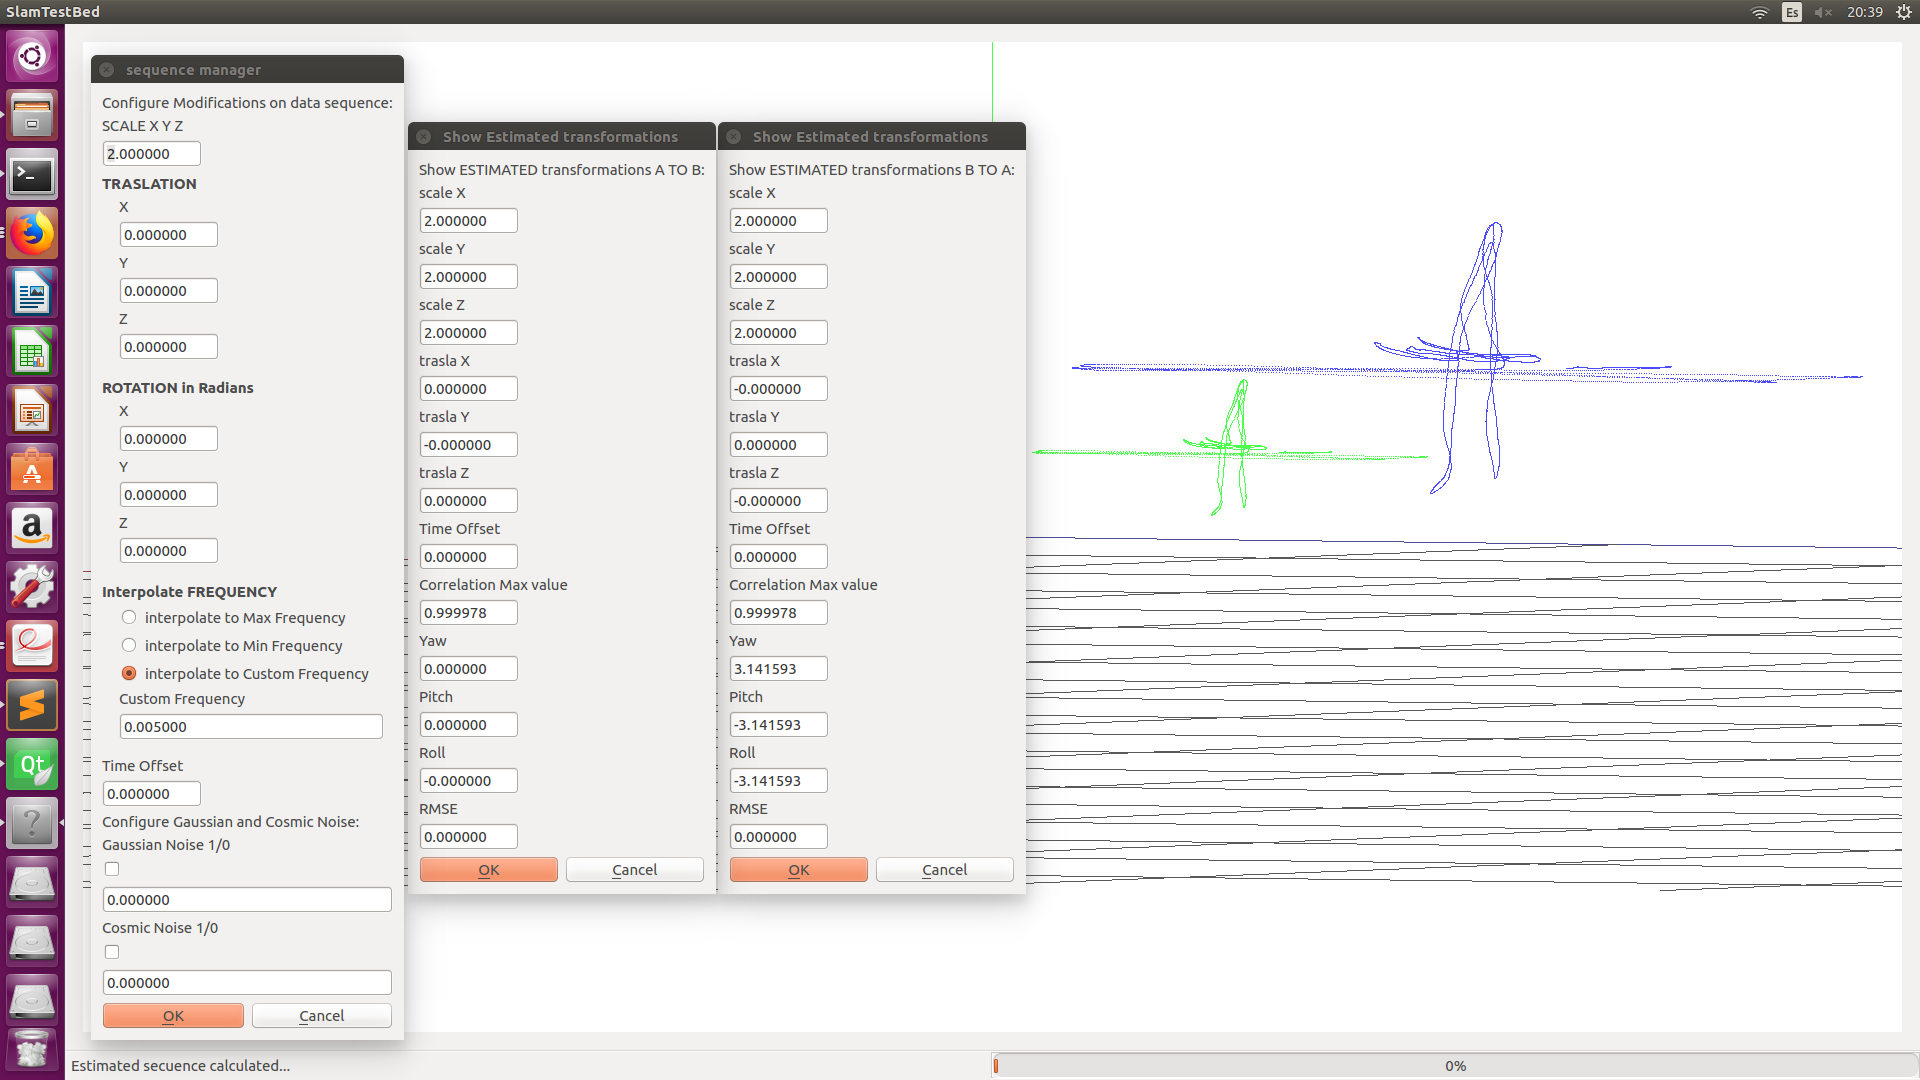
\includegraphics[height=14.0cm,width=18.0cm]{img/cap6/Escala_abba.png}
\hspace{0.5cm}

%\end{center}

\caption{Resultados de la estimación tras una transformación de un cambio de escala.}
\end{figure}

La Figura 5.1 muestra los resultados de la estimación tras una transformación de un cambio de escala. Se aprecia en la captura de pantalla, cómo el dataset transformado es más grande que el dataset original. Como se puede observar el RMSE es 0.0 y el valor de la escala estimada coincide con el valor de la transformación de escala, en este caso es 2.0.

\subsection{Pruebas con traslación}

\begin{figure}[H]
%\begin{center}
\label{fig:traslaTest}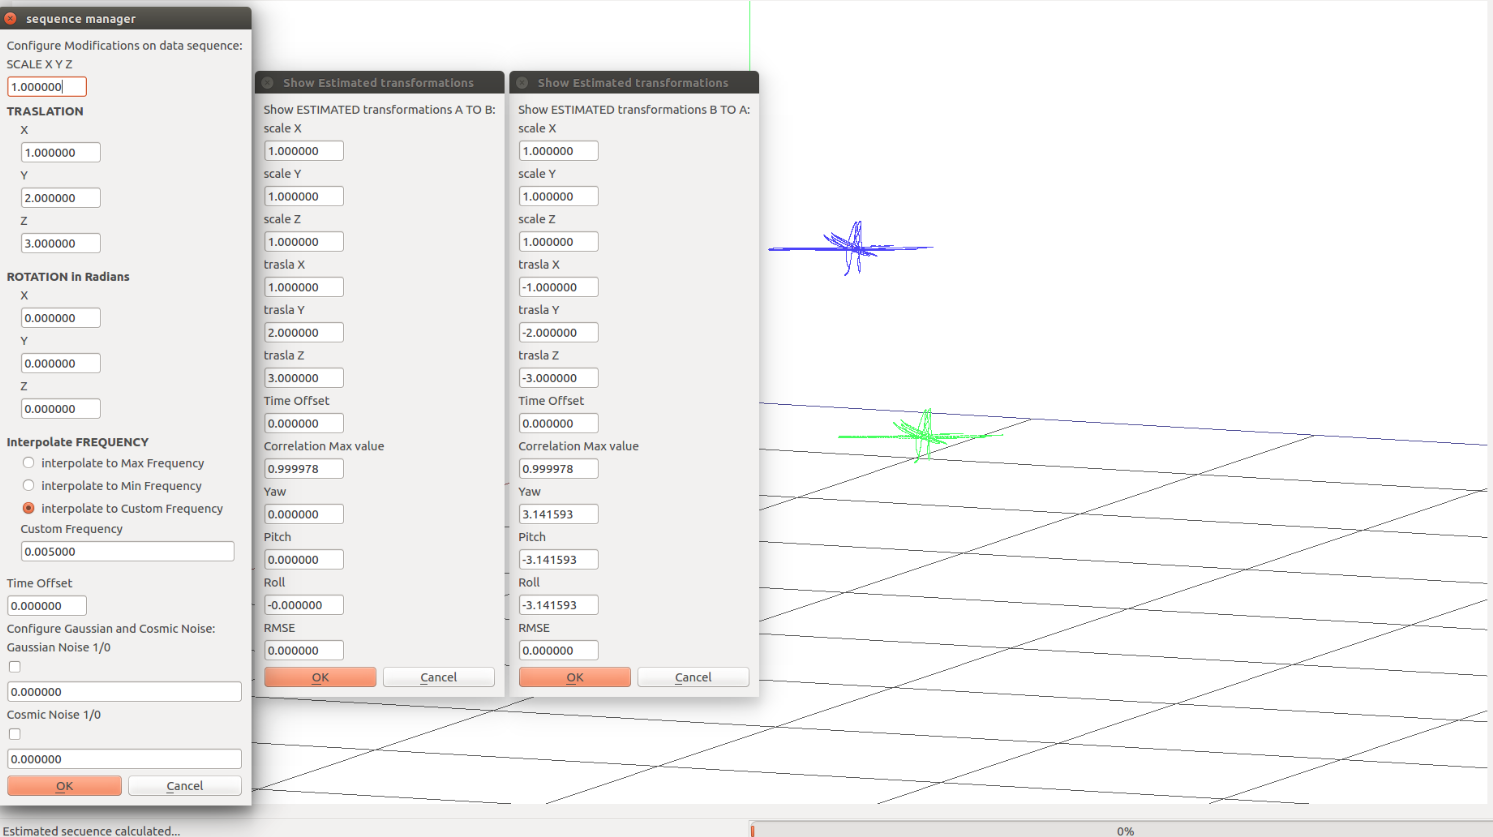
\includegraphics[height=14.0cm,width=18.0cm]{img/cap6/Traslation_abba.png}
\hspace{0.5cm}

%\end{center}

\caption{Resultados de la estimación de un cambio de traslación.}
\end{figure}


La Figura 5.2 muestra los resultados de la estimación tras realizar una traslación en el dataset original. Como puede observarse el RMSE es 0.0, y gráficamente el dataset transformado y estimado coinciden en cada posición 3D. Es por este motivo por el que hay ausencia de puntos rojos en la representación 3D. Hay que recordar que el dataset estimado se presenta con puntos rojos. Cuando la estimación no es buena, el dataset transformado y estimado no coincidirán y podremos ver en pantalla los puntos rojos, allí donde precisamente no coincidan dataset estimado. En cuanto a los valores de la traslación estimada puede verse que coinciden con la transformación realizada.

\subsection{Prueba de rotación}

\begin{figure}[H]
%\begin{center}
\label{fig:rotationTest}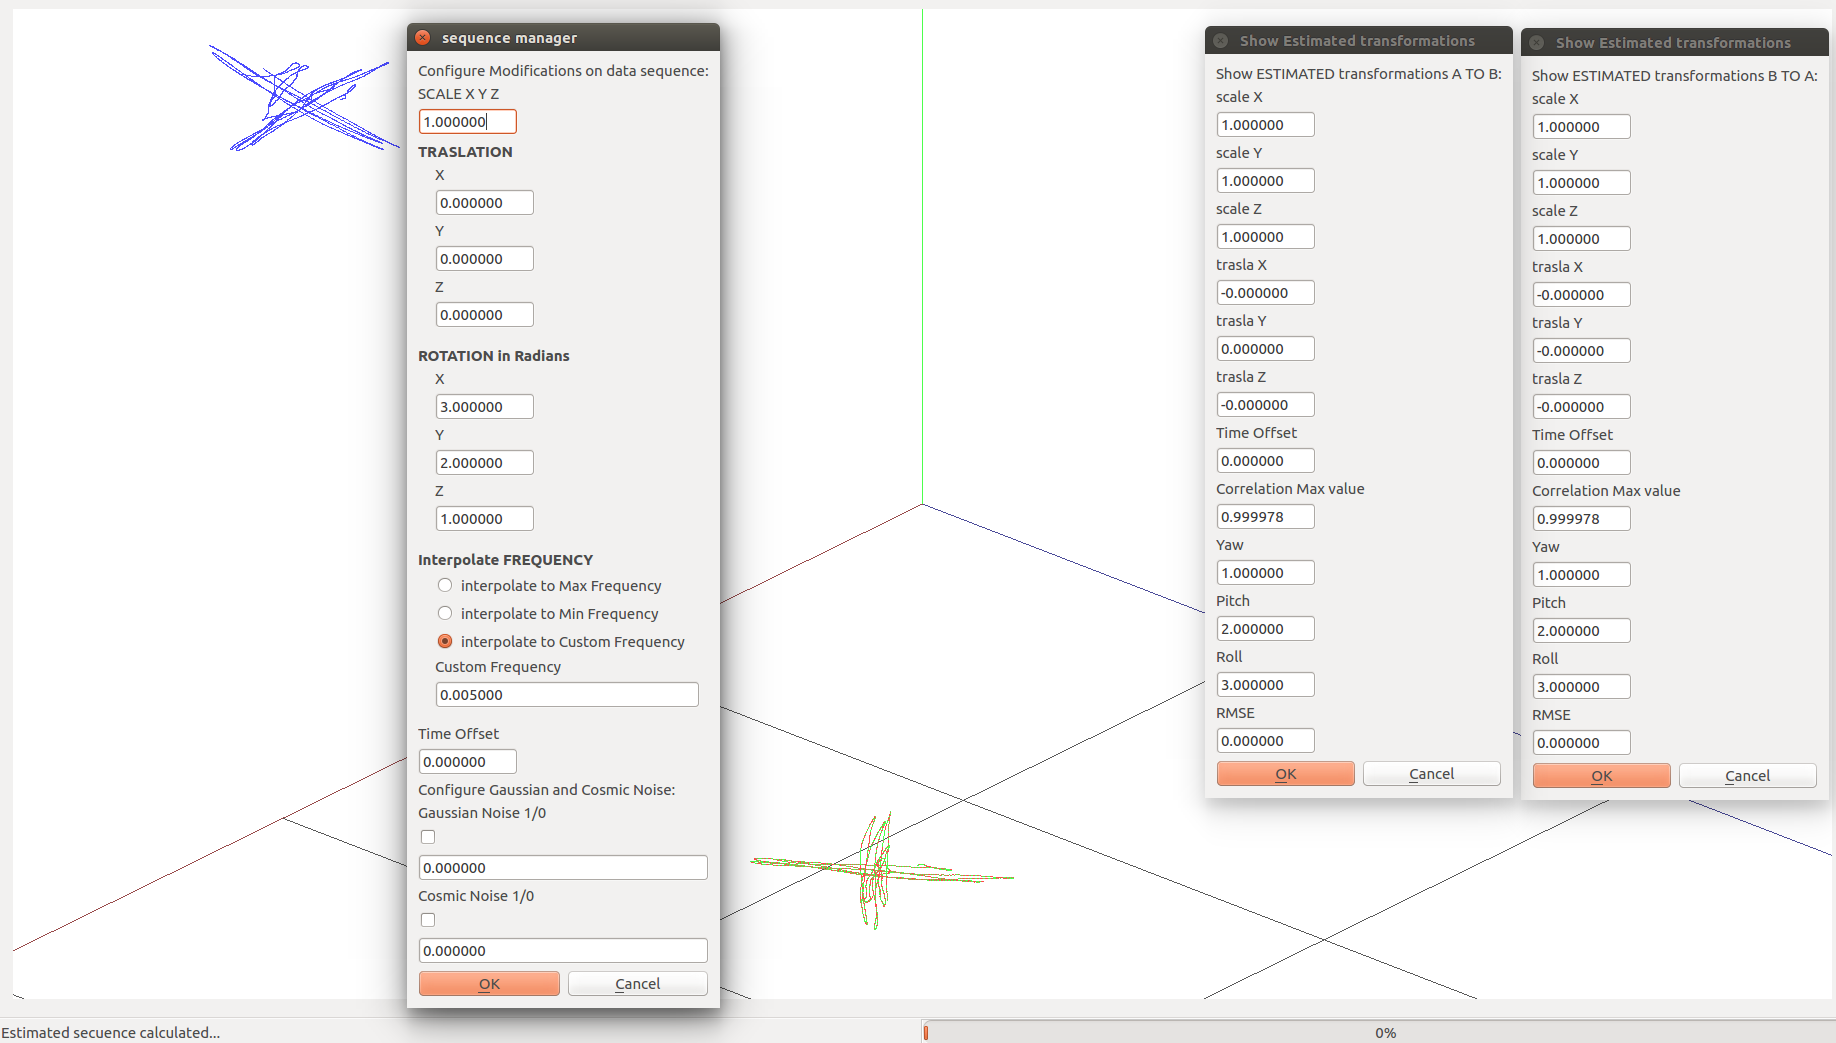
\includegraphics[height=14.0cm,width=18.0cm]{img/cap6/Rotation_ab_ba.png}
\hspace{0.5cm}

%\end{center}

\caption{Resultados de la estimación de un cambio de rotación.}
\end{figure}

En la Figura 5.3 podremos observar el dataset original en verde, y el dataset transformado tras aplicar una rotación. La rotación se especifica en radianes. Como puede observarse, el error (RMSE) es mínimo 0.0. Se puede comprobar que la rotación realizada en los ejes X,Y,Z en la transformación ha sido respectivamente de 3.0, 2.0 y 1.0 radianes, y en la estimación estos valores coinciden.


%%%%%%%%%%%%%%%%%%%%%   TRANSFORMACIONES EN PAREJAS 
\section{Pruebas de transformaciones en parejas}
En este apartado mostraremos imágenes del módulo GUI con varias pruebas de dos  transformaciones simultáneas y se han estimado dichas transformaciones con SLAMTestbed.
En todas las transformaciones se ha realizado la transformación de frecuencias al valor 0.005 milisegundos para ambos datasets. 

Una vez que en la sección anterior se ha validado el correcto comportamiento de SLAMTestbed cuando se le presentaban transformaciones individuales, un paso más para validar su robustez es presentarle varias transformaciones simultáneas que ponen a prueba las posibles interferencias entre sus diferentes módulos de estimación, por si estuvieran acoplados. En cada prueba las transformaciones se realizaran por parejas.
Las transformaciones  a validar serán:
\begin{itemize}
 \item{Escala y Traslación}
 \item{Escala y Rotación}
 \item{Escala y Offset temporal}
 \item{Escala y Ruido gaussiano}
 \item{Escala y Ruido cósmico}

 \item{Traslación y Rotación}
 \item{Traslación y Offset Temporal}
 \item{Traslación y Ruido Gaussiano}
 \item{Traslación y Ruido Cósmico}

 \item{Rotación y Offset Temporal}
 \item{Rotación y Ruido Gaussiano}
 \item{Rotación y Ruido Cósmico}
\end{itemize}





\subsection{Pruebas con traslación y escala}

\begin{figure}[H]
\begin{center}
\label{fig:traslaEscalaTest}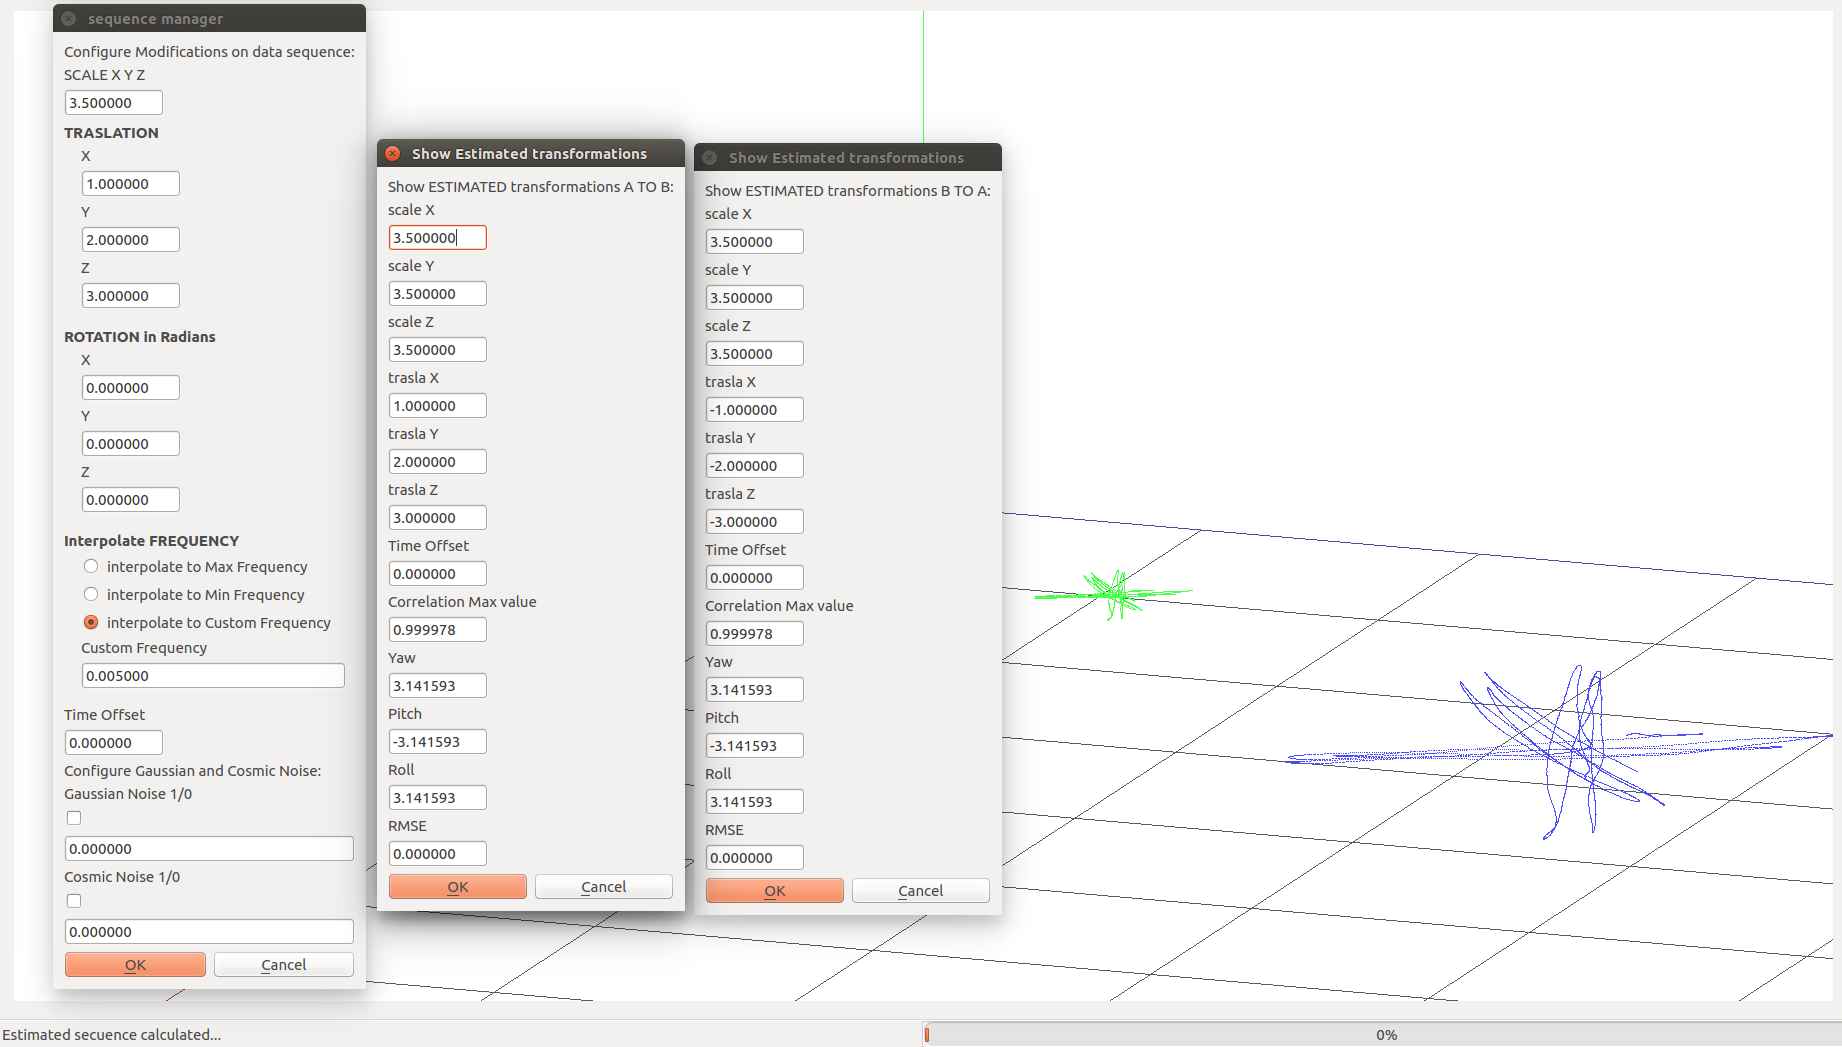
\includegraphics[height=14.0cm,width=18.0cm]{img/cap6/Escala_Traslacion_abba.png}
\hspace{0.5cm}

\end{center}

\caption{Resultados de la estimación de un cambio de escala y traslación .}
\end{figure}

En la Figura 5.4 se muestra en color verde el dataset \textit{groundtruth} y en azul el mismo dataset tras realizarle un par de transformaciones en escala y traslación.
En la ventana de la derecha se muestran los resultados de la transformación estimada, que coincide con la transformación doble realizada, además el RMSE es 0.

El dataset estimado se pinta en color rojo, pero en este caso la estimación es tan buena que coincide con el dataset transformado y no se aprecia ningún punto rojo.
En este caso la transformación realizada es de escala y traslación. Se puede comprobar que la estimación realizada es correcta ya que coinciden los valores de la escala y traslación estimados.

\subsection{Pruebas con escala y rotación}

\begin{figure}[H]
\begin{center}
\label{fig:escalaRotationTest}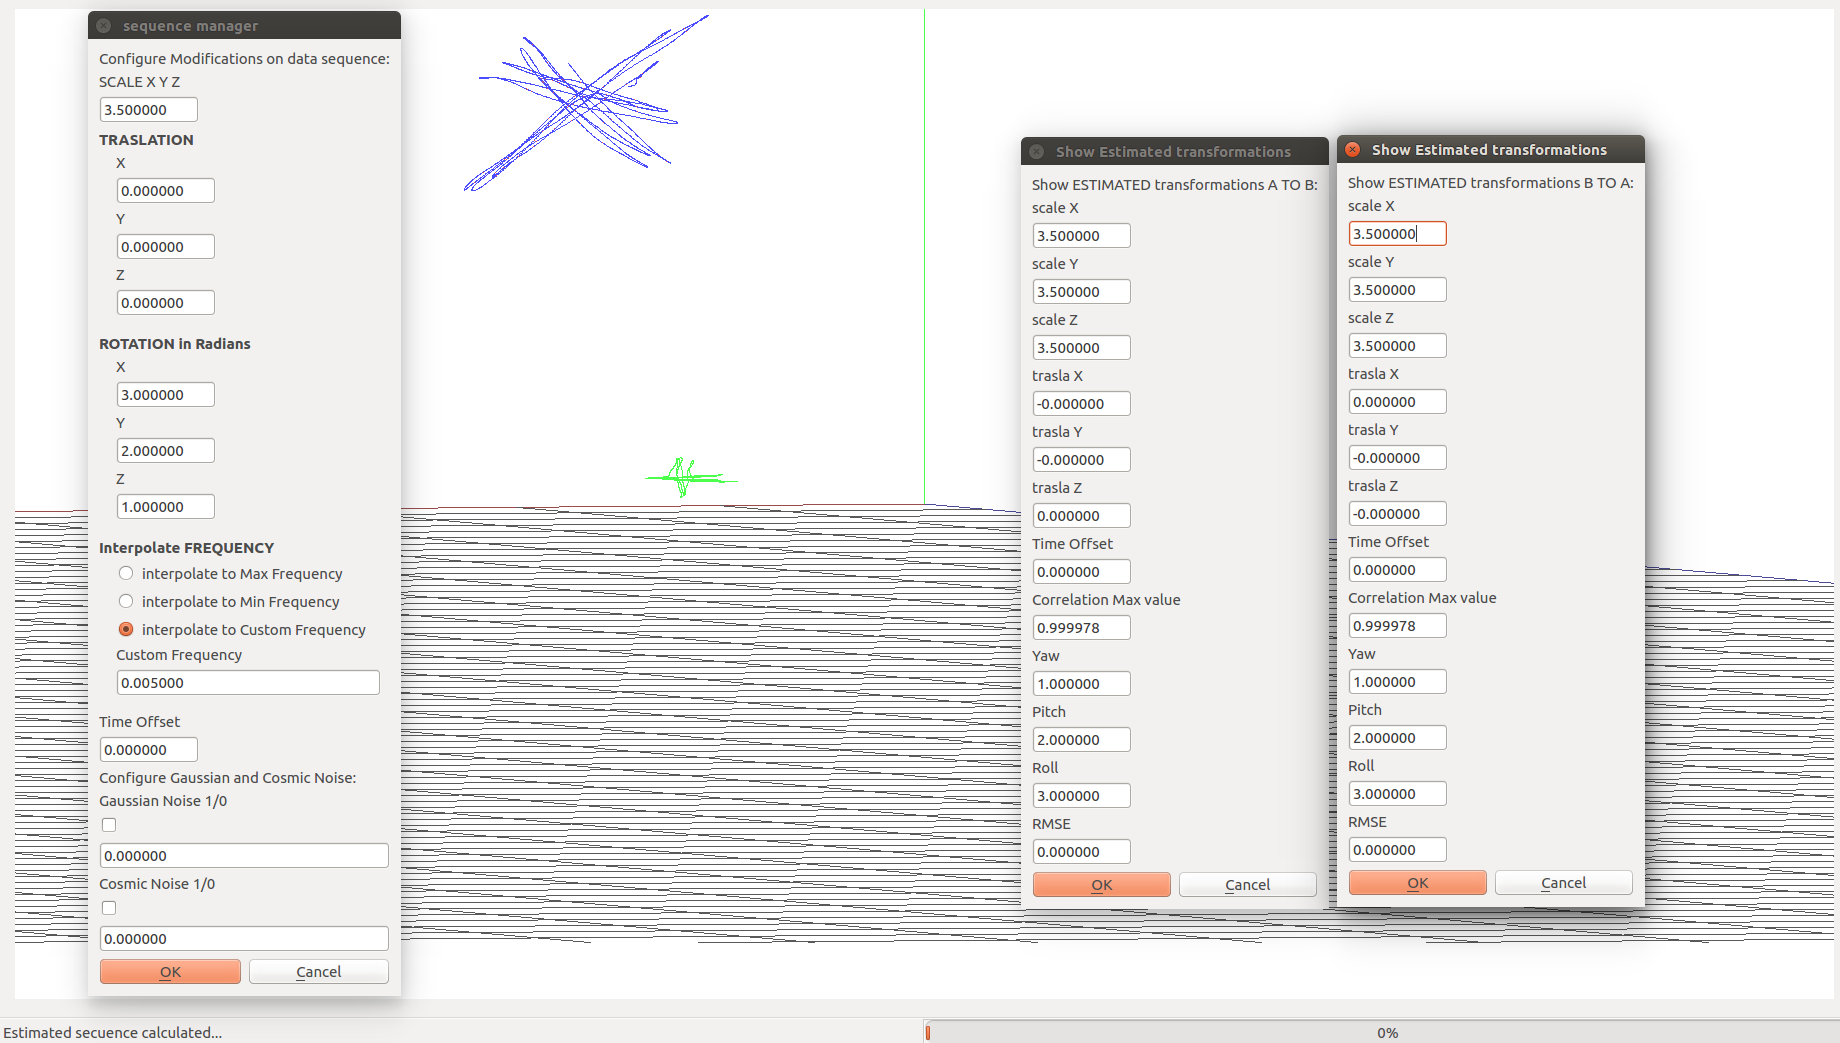
\includegraphics[height=14.0cm,width=18.0cm]{img/cap6/Escala_Rotation_abba.png}
\hspace{0.5cm}

\end{center}

\caption{Resultados de la estimación de un cambio de escala y rotación.}
\end{figure}
En la Figura 5.5 podemos ver los resultados de aplicar otras 2 transformaciones simultáneas sobre el dataset original. En este caso una transformación en escala y otra de rotación. Tras realizar la estimación, el error medido entre el dataset estimado y el dataset transformado es 0.0. Por tanto podemos decir que la estimación es exacta a la transformación realizada sobre el dataset original.

\subsection{Pruebas con escala y offset temporal}
\begin{figure}[H]
\begin{center}
\label{fig:opciones de View}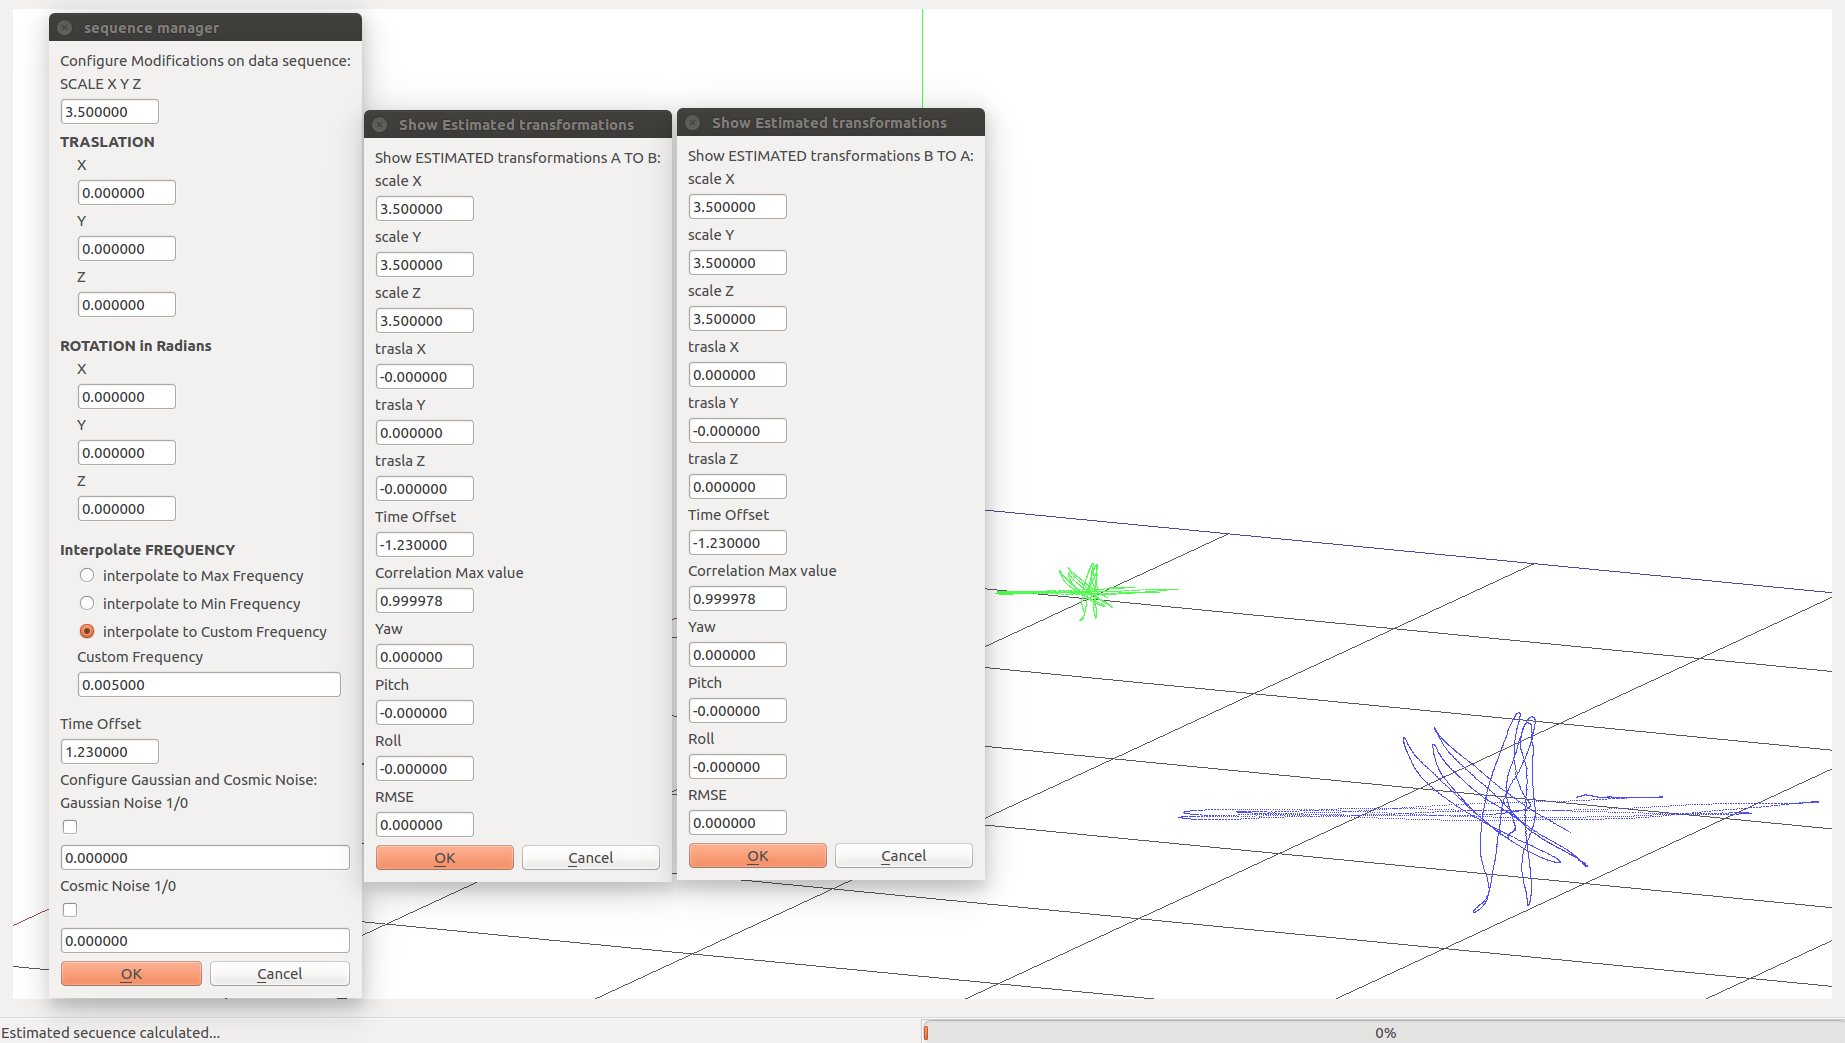
\includegraphics[height=14.0cm,width=18.0cm]{img/cap6/Escala_Offset_abba.png}
\hspace{0.5cm}

\end{center}

\caption{Resultados de la estimación de un cambio de escala y offset.}
\end{figure}

En la Figura 5.6 al dataset original (color verde) se le ha aplicado un par de transformaciones (en escala y con offset), dando lugar al conjunto azul. También la estimación es buena, ya que el error RMSE da como resultado 0.0 y el cálculo del offset estimado coincide con el valor del offset que se ha aplicado en la transformación, salvo con signo negativo.

\subsection{Pruebas con escala y ruido gaussiano}

\begin{figure}[H]
\begin{center}
\label{fig:opciones de View}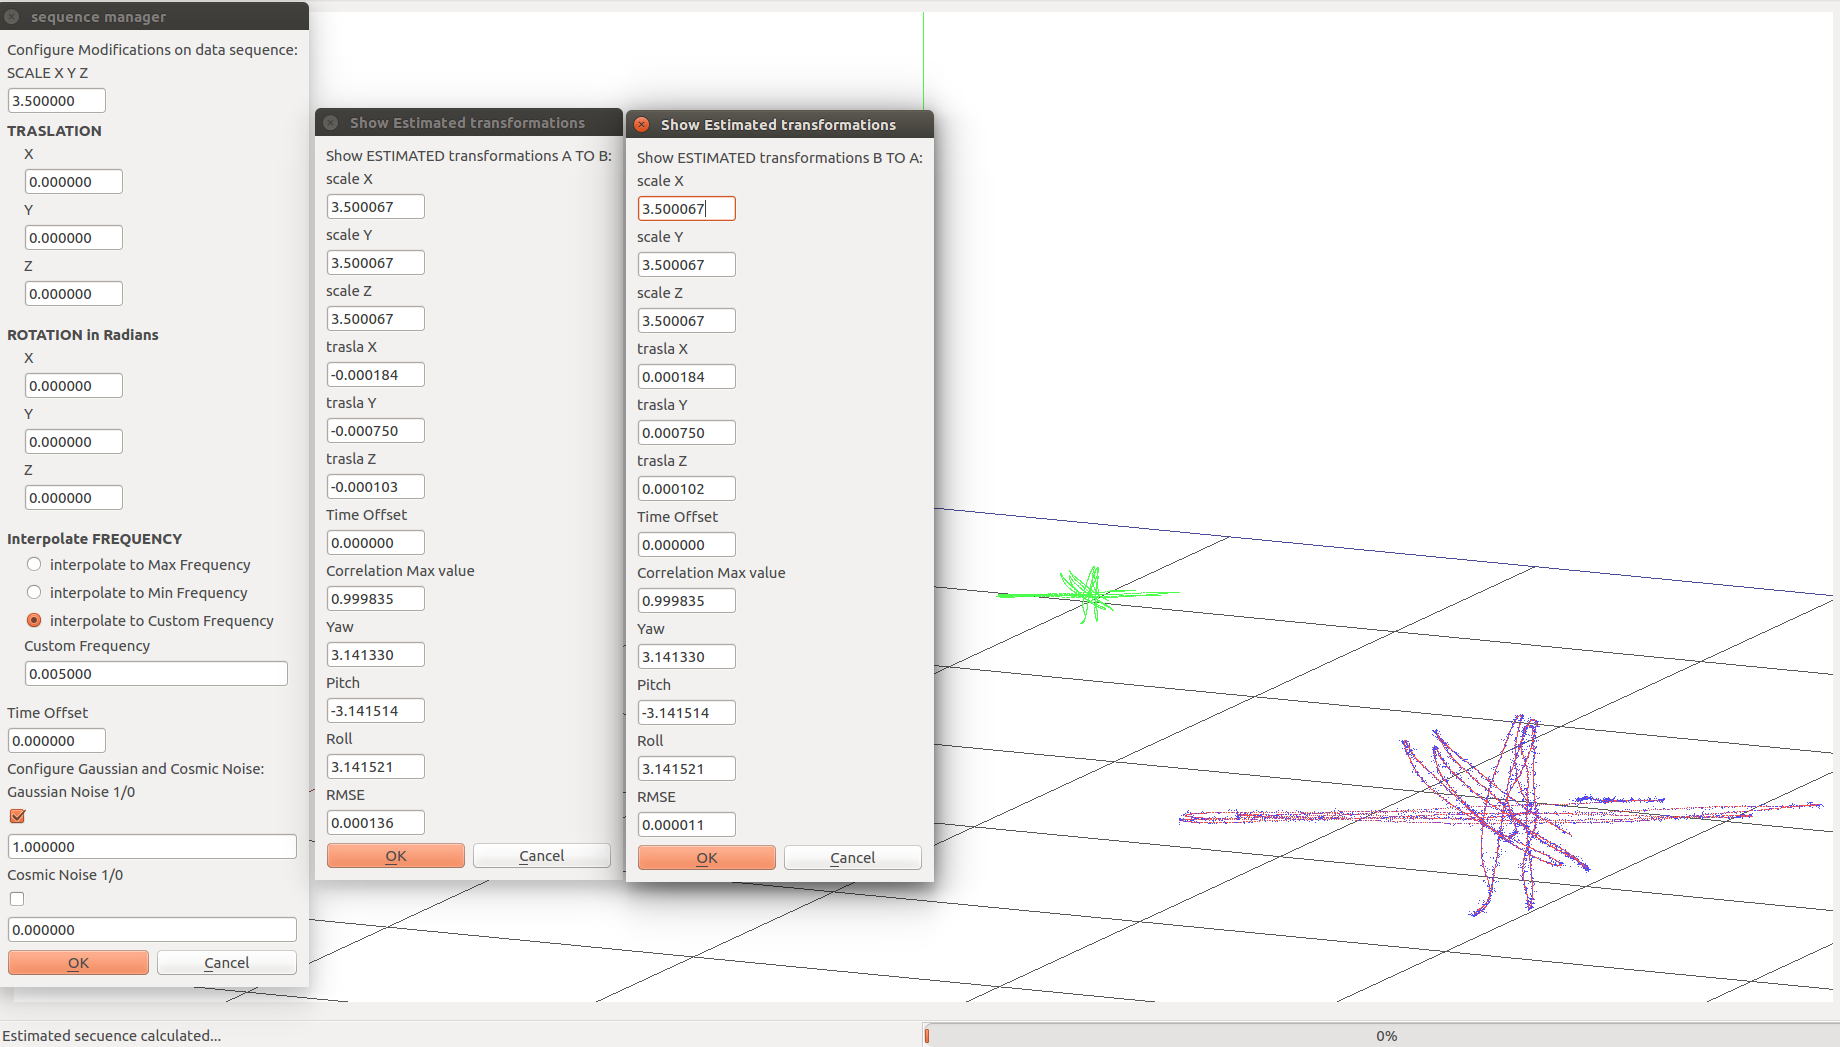
\includegraphics[height=14.0cm,width=18.0cm]{img/cap6/Escala_GaussNoise_abba.png}
\hspace{0.5cm}

\end{center}

\caption{Resultados de la estimación de un cambio de escala y ruido gaussiano .}
\end{figure}

En la Figura 5.7, se ha aplicado sobre el dataset original un cambio de escala y además se le ha añadido ruido gaussiano, como puede verse en el dataset resultante (color azul). Las estimaciones obtenidas son buenas, pero el error RMSE calculado entre el dataset transformado y el dataset estimando ya no es 0.0, sino 0.000136. Esta falta de precisión puede apreciarse a simple vista, ya que como el dataset estimado carece de ruido gaussiano, los puntos del dataset estimado no coinciden exactamente con los puntos del dataset transformado, y por tanto ahora sí podemos ver buena parte de los puntos del dataset estimado (color rojo).
También se observa un error mínimo en la estimación de escala, 3.500067 cuando debería ser 3.5, y la traslación en X,Y,Z debería ser 0.0 y sin embargo hay un error mínimo de 4 decimales.

Esta coincidencia valida el funcionamiento de SLAMTestbed en presencia de ruido gaussiano en las secuencias que será lo habitual en el uso real.

\subsection{Pruebas con escala y ruidos gaussiano y cósmico}
\begin{figure}[H]
\begin{center}
\label{fig:opciones de View}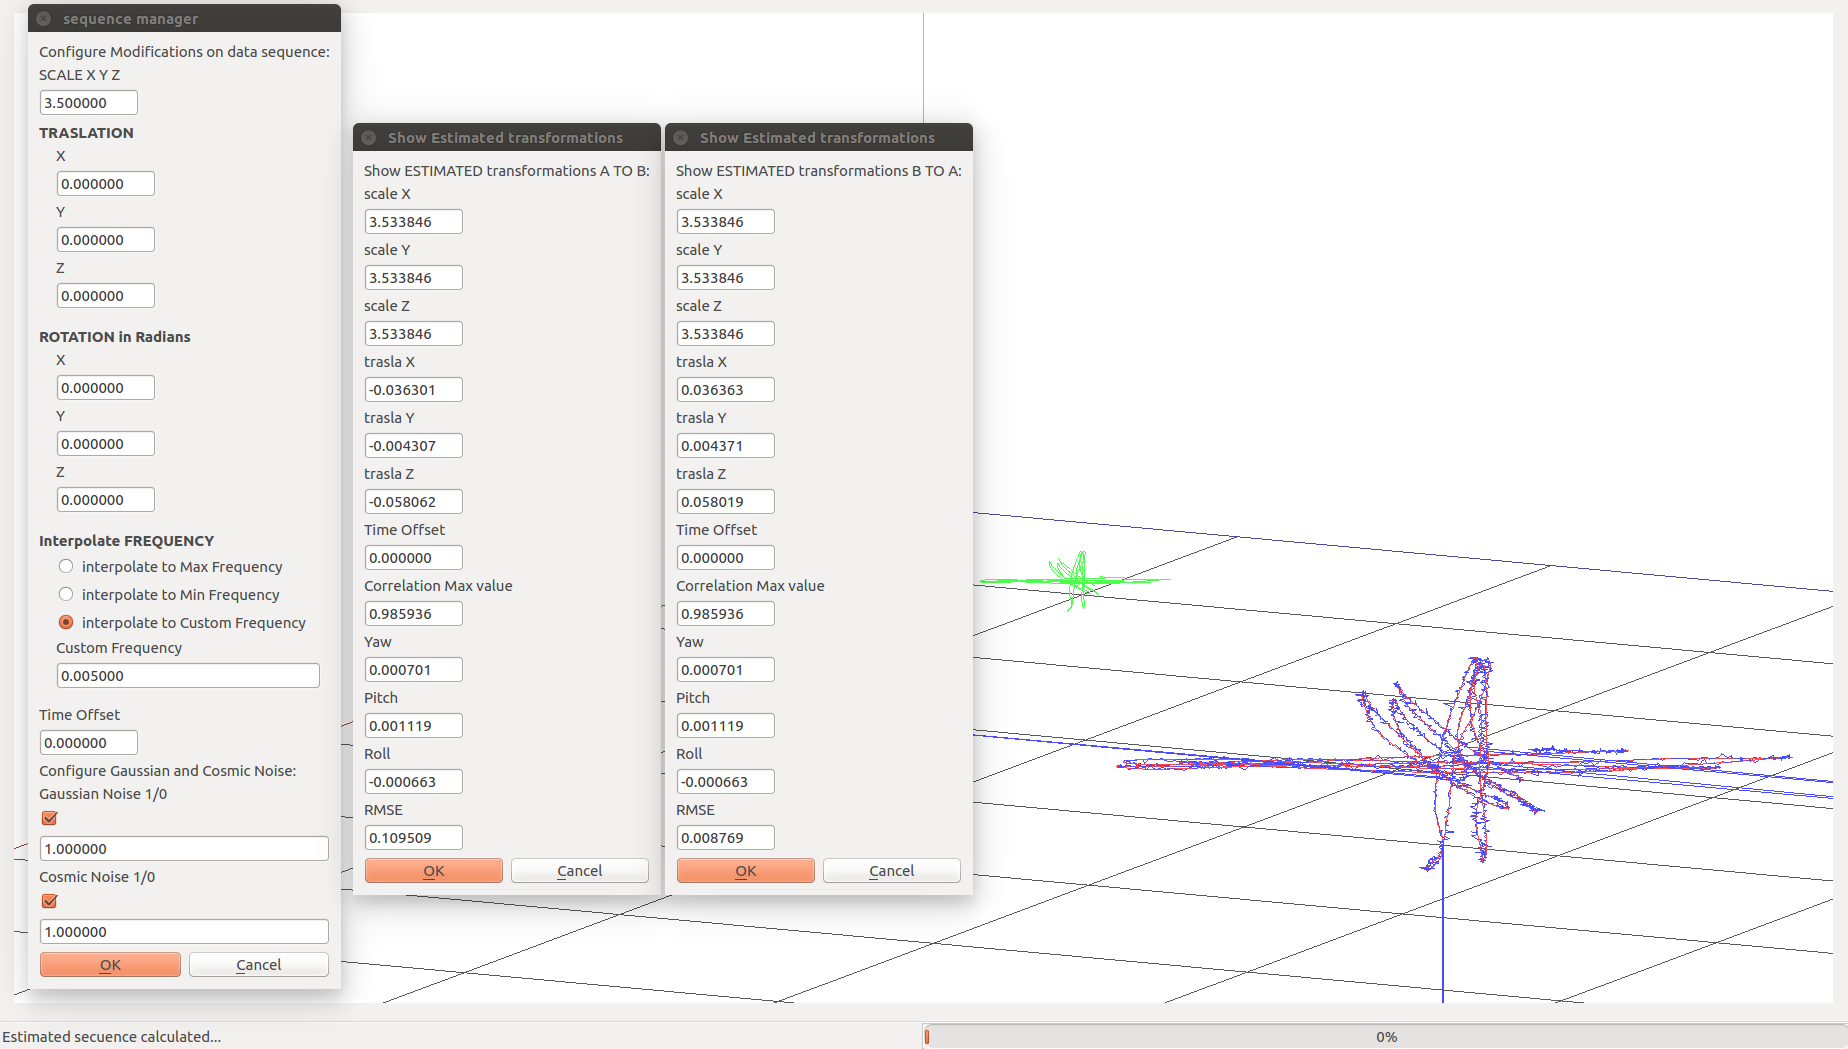
\includegraphics[height=14.0cm,width=18.0cm]{img/cap6/Escala_GaussCosmicNoise_abba.png}
\hspace{0.5cm}

\end{center}

\caption{Resultados de la estimación de un cambio de escala con ruido gaussiano y cósmico}
\end{figure}

En la Figura 5.8 se ha aplicado sobre el dataset original un cambio de escala más ruido gaussiano y cósmico. Al tener ahora ruido cósmico, en algunos puntos del dataset transformado aparecen unos valores muy superiores a la media, estos valores desorbitados harán que aumente notablemente el error entre el dataset transformado y el dataset estimado.
Para este experimento el valor RMSE es de 0.109 (en sentido A-B) y de 0.008 (en sentido B-A). Aunque puede observarse que aún así, la posición de los puntos del dataset estimado coincide con la posición de los puntos del dataset transformado.


\subsection{Pruebas con traslación y roatación simultáneas}
\begin{figure}[H]
\begin{center}
\label{fig:opciones de View}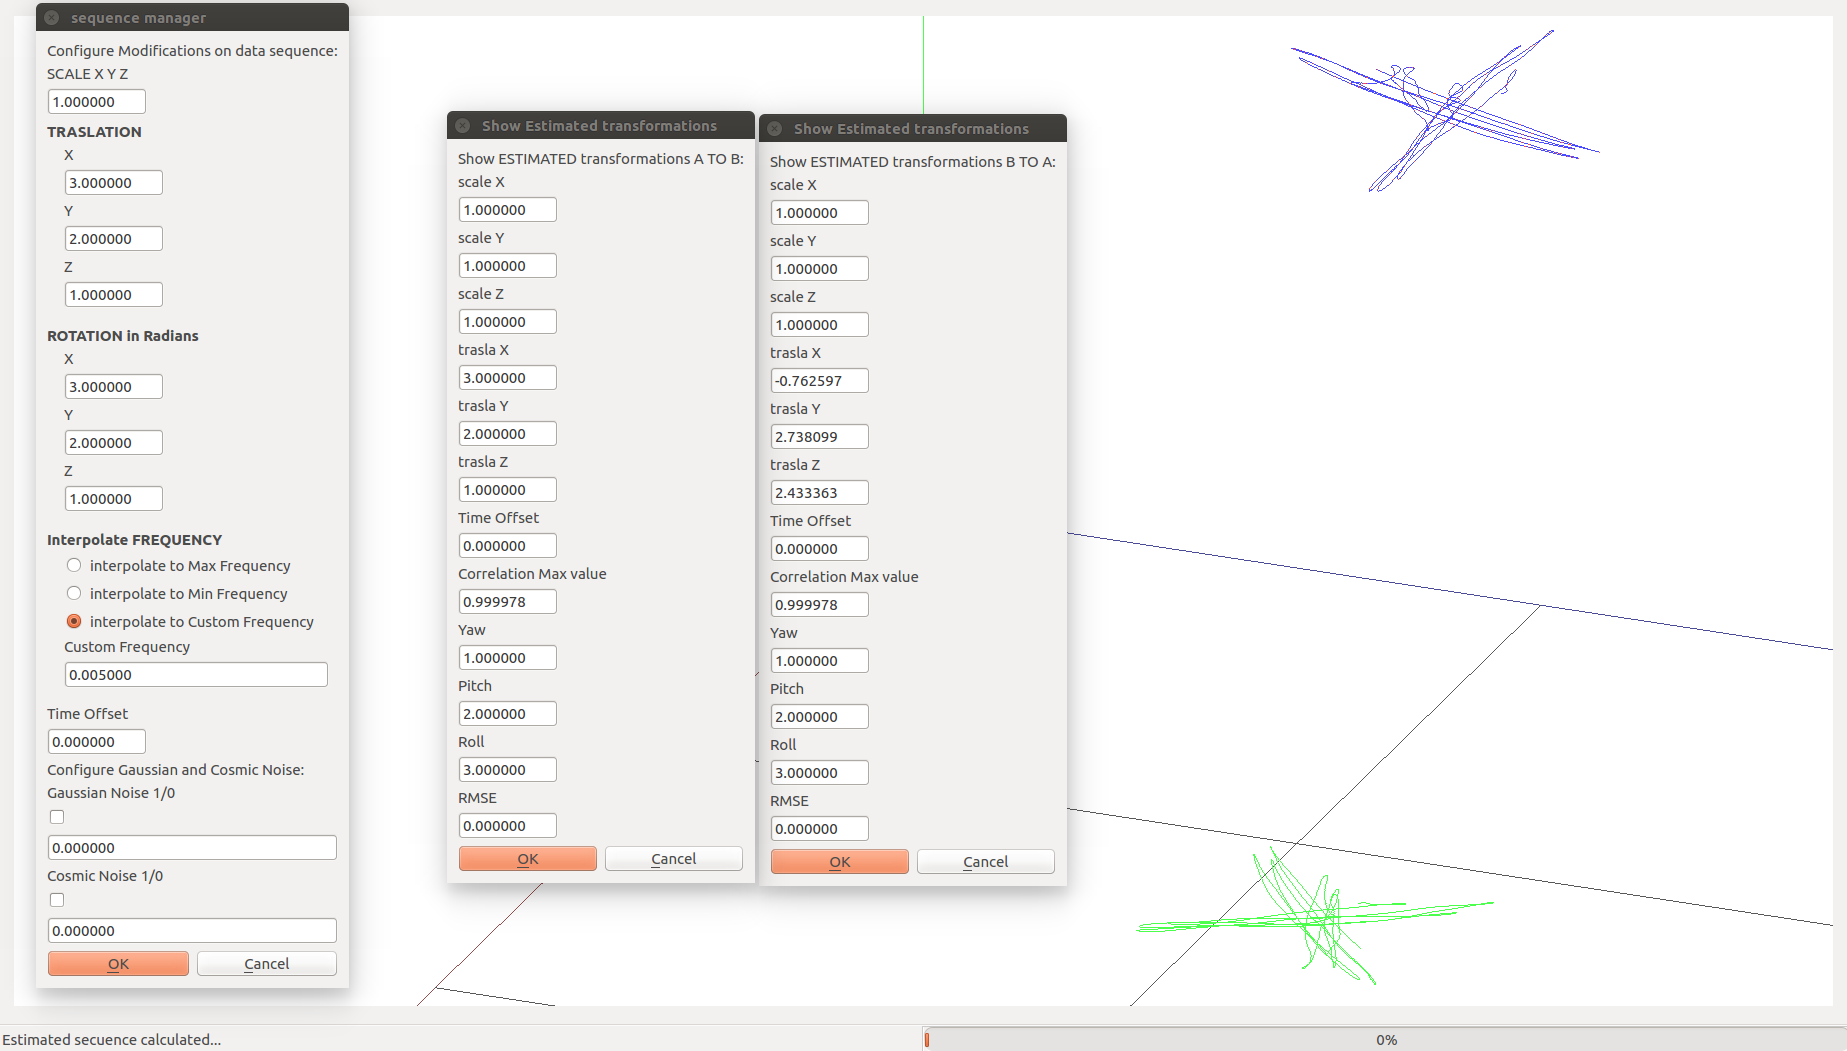
\includegraphics[height=14.0cm,width=18.0cm]{img/cap6/Trasla_Rota_abba.png}
\hspace{0.5cm}

\end{center}

\caption{Resultados de la estimación de un cambio de traslación y rotación.}
\end{figure}

En la Figura 5.9 se han aplicado 2 transformaciones sobre el dataset original: una traslación y una rotación.
La estimación de la traslación y la rotación coinciden con los valores de las transformaciones. El error calculado entre el dataset estimado y el dataset transformado es 0.0 lo que refleja que SLAMTestbed está estimando correctamente la relación ente las dos secuencias.

\subsection{Pruebas con traslación y offset temporal}

\begin{figure}[H]
\begin{center}
\label{fig:opciones de View}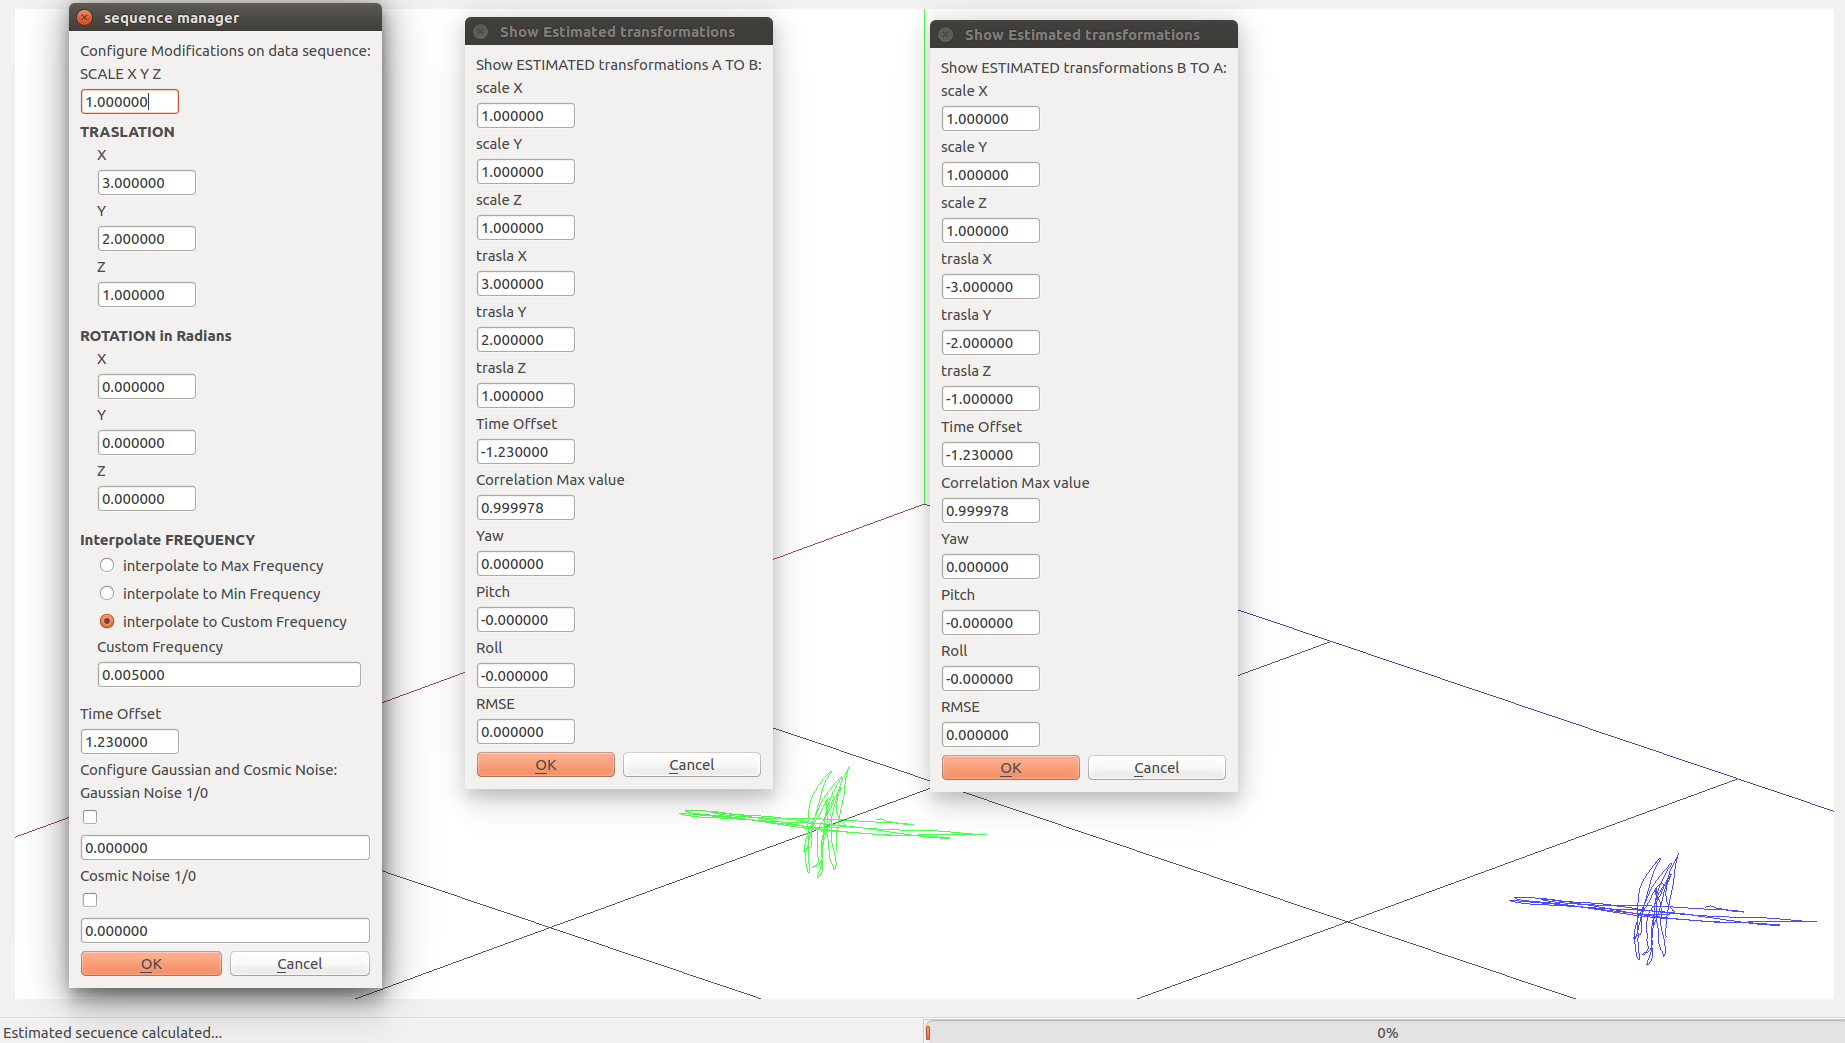
\includegraphics[height=14.0cm,width=18.0cm]{img/cap6/Trasla_Offset_abba.png}
\hspace{0.5cm}

\end{center}

\caption{Resultados de la estimación de un cambio de traslación y offset.}
\end{figure}
En la Figura 5.10 al dataset original (color verde) se le ha aplicado un par de transformaciones (traslación y con offset), dando lugar al dataset transformado (conjunto de puntos de color azul). También aquí la estimación es buena, ya que el error RMSE da como resultado 0.0 y el cálculo del offset  coincide con el valor del offset que se ha aplicado en la transformación, salvo con signo negativo.

\subsection{Pruebas con traslación y ruido gaussiano}

\begin{figure}[H]
\begin{center}
\label{fig:opciones de View}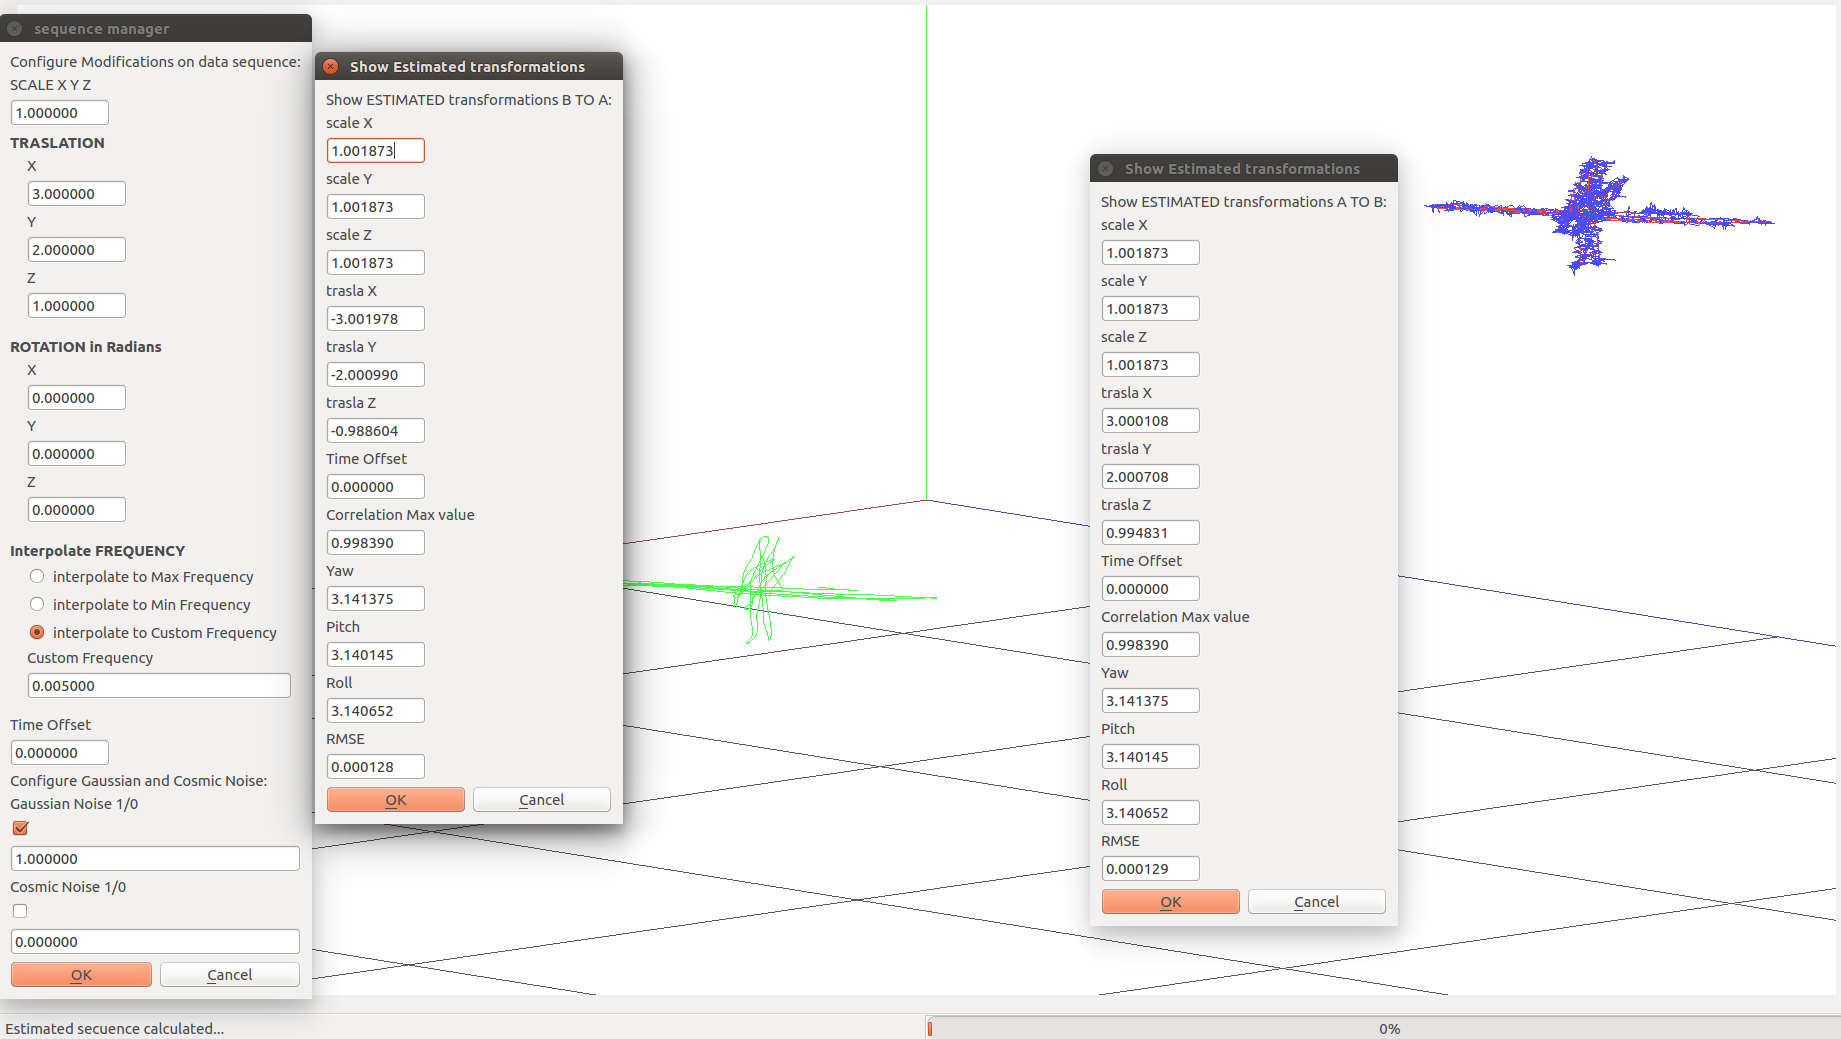
\includegraphics[height=14.0cm,width=18.0cm]{img/cap6/Trasla_GaussNoise_abba.png}
\hspace{0.5cm}

\end{center}

\caption{Resultados de la estimación de un cambio de traslación y ruido gaussiano.}
\end{figure}
En la Figura 5.11 se ha aplicado sobre el dataset original un cambio de traslación y además se le ha añadido ruido gaussiano, como puede verse en el dataset resultante (color azul). Las estimaciones obtenidas son buenas, pero el error RMSE calculado entre el dataset transformado y el dataset estimado ya no es 0.0, sino 0.00128. Esta falta de precisión puede apreciarse a simple vista en el interfaz gráfico, ya que como el dataset estimado carece de ruido gaussiano, los puntos del dataset estimado no coinciden exactamente con los puntos del dataset transformado, y por tanto ahora sí podemos ver buena parte de los puntos del dataset estimado (color rojo).
Mientras ese RMSE se mantenga en valores bajos es aceptable puesto que es natural incurrir en cierto error no nulo cuando hay ruido en la secuencia de entrada.

\subsection{Pruebas con traslación y ruidos gaussiano y cósmico}
\begin{figure}[H]
\begin{center}
\label{fig:opciones de View}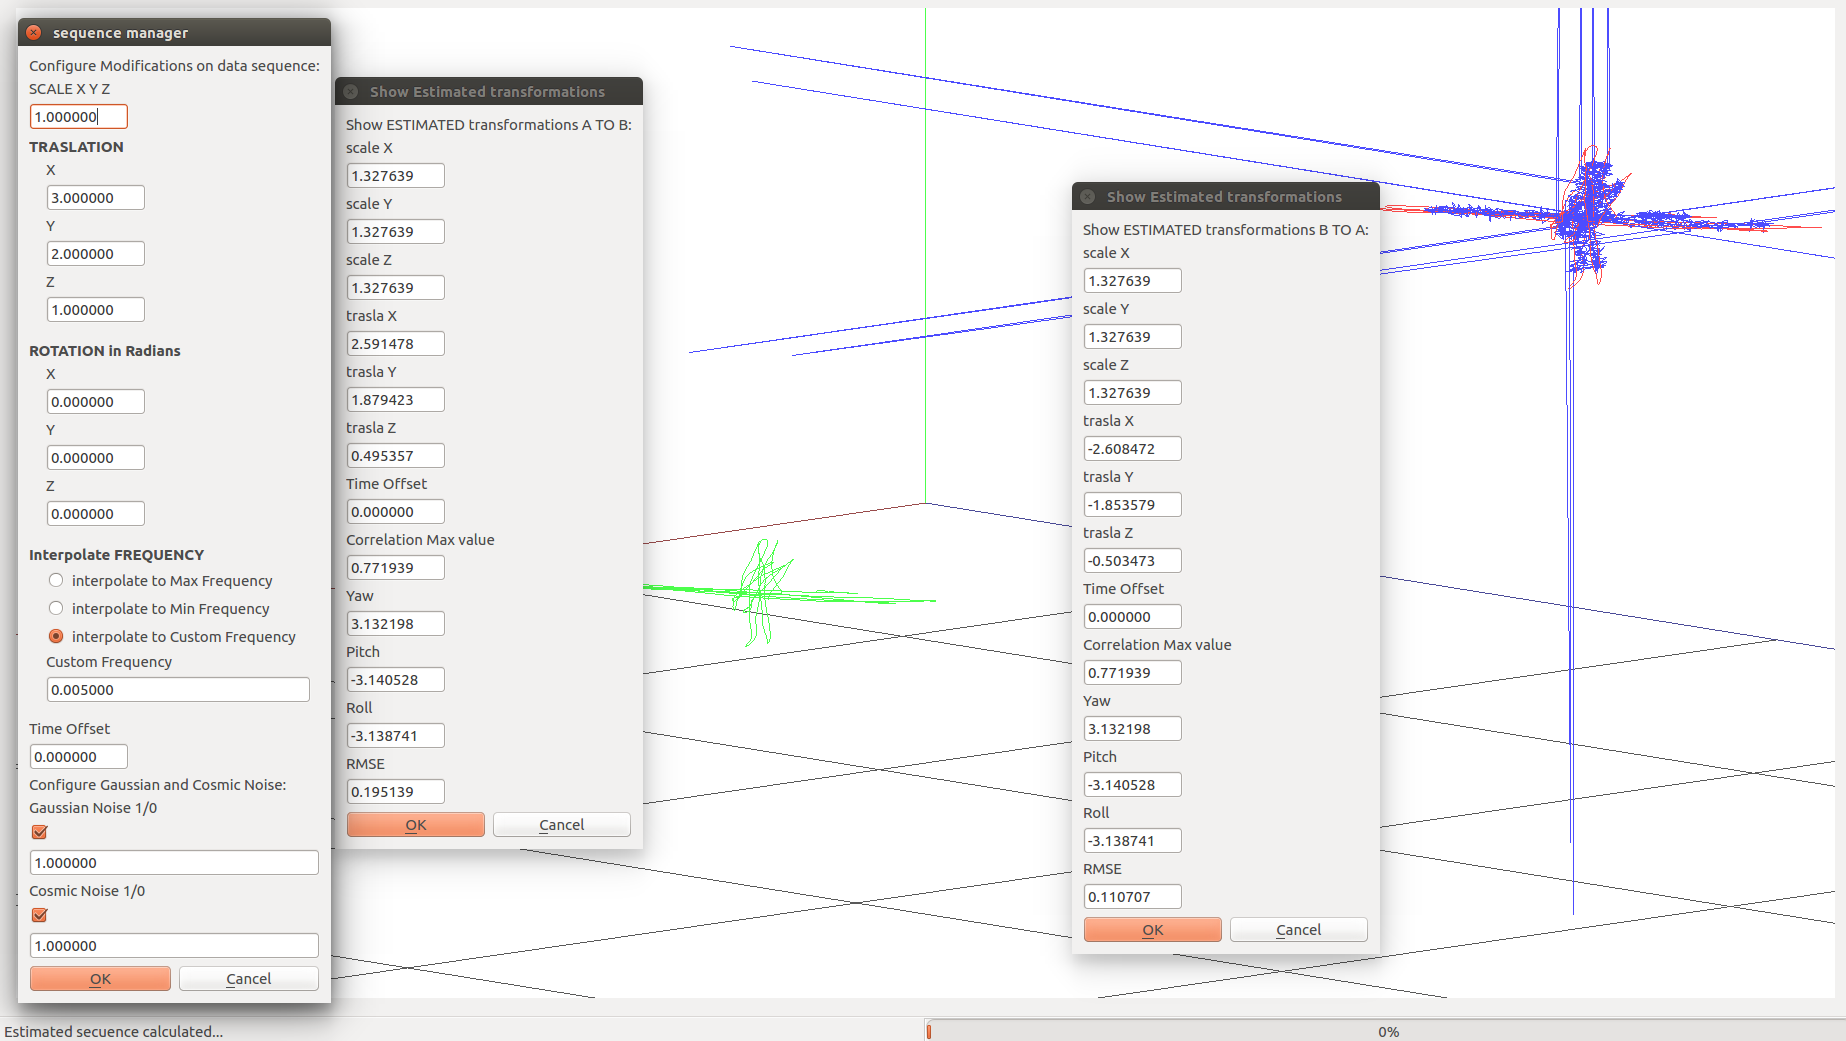
\includegraphics[height=14.0cm,width=18.0cm]{img/cap6/Trasla_GaussianCosmicNoise_abba.png}
\hspace{0.5cm}

\end{center}

\caption{Resultados de la estimación de un cambio de traslación, ruido cósmico y gaussiano}
\end{figure}

En la Figura 5.12 se ha aplicado sobre el dataset original un cambio de traslación más ruido gaussiano y cósmico. Al añadir ruido cósmico, en algunos puntos del dataset transformado aparecen unos valores muy superiores al rango de valores del dataset, dando lugar a la aparición de \textit{outliers} que hacen que aumente notablemente el error entre el dataset transformado y el dataset estimado. Para este experimento, el valor RMSE es de 0.12. Puede observarse que aún así, la posición de los puntos del dataset estimado coincide con la posición de los puntos del dataset transformado.


\subsection{Pruebas con rotación y offset temporal}
\begin{figure}[H]
\begin{center}
\label{fig:opciones de View}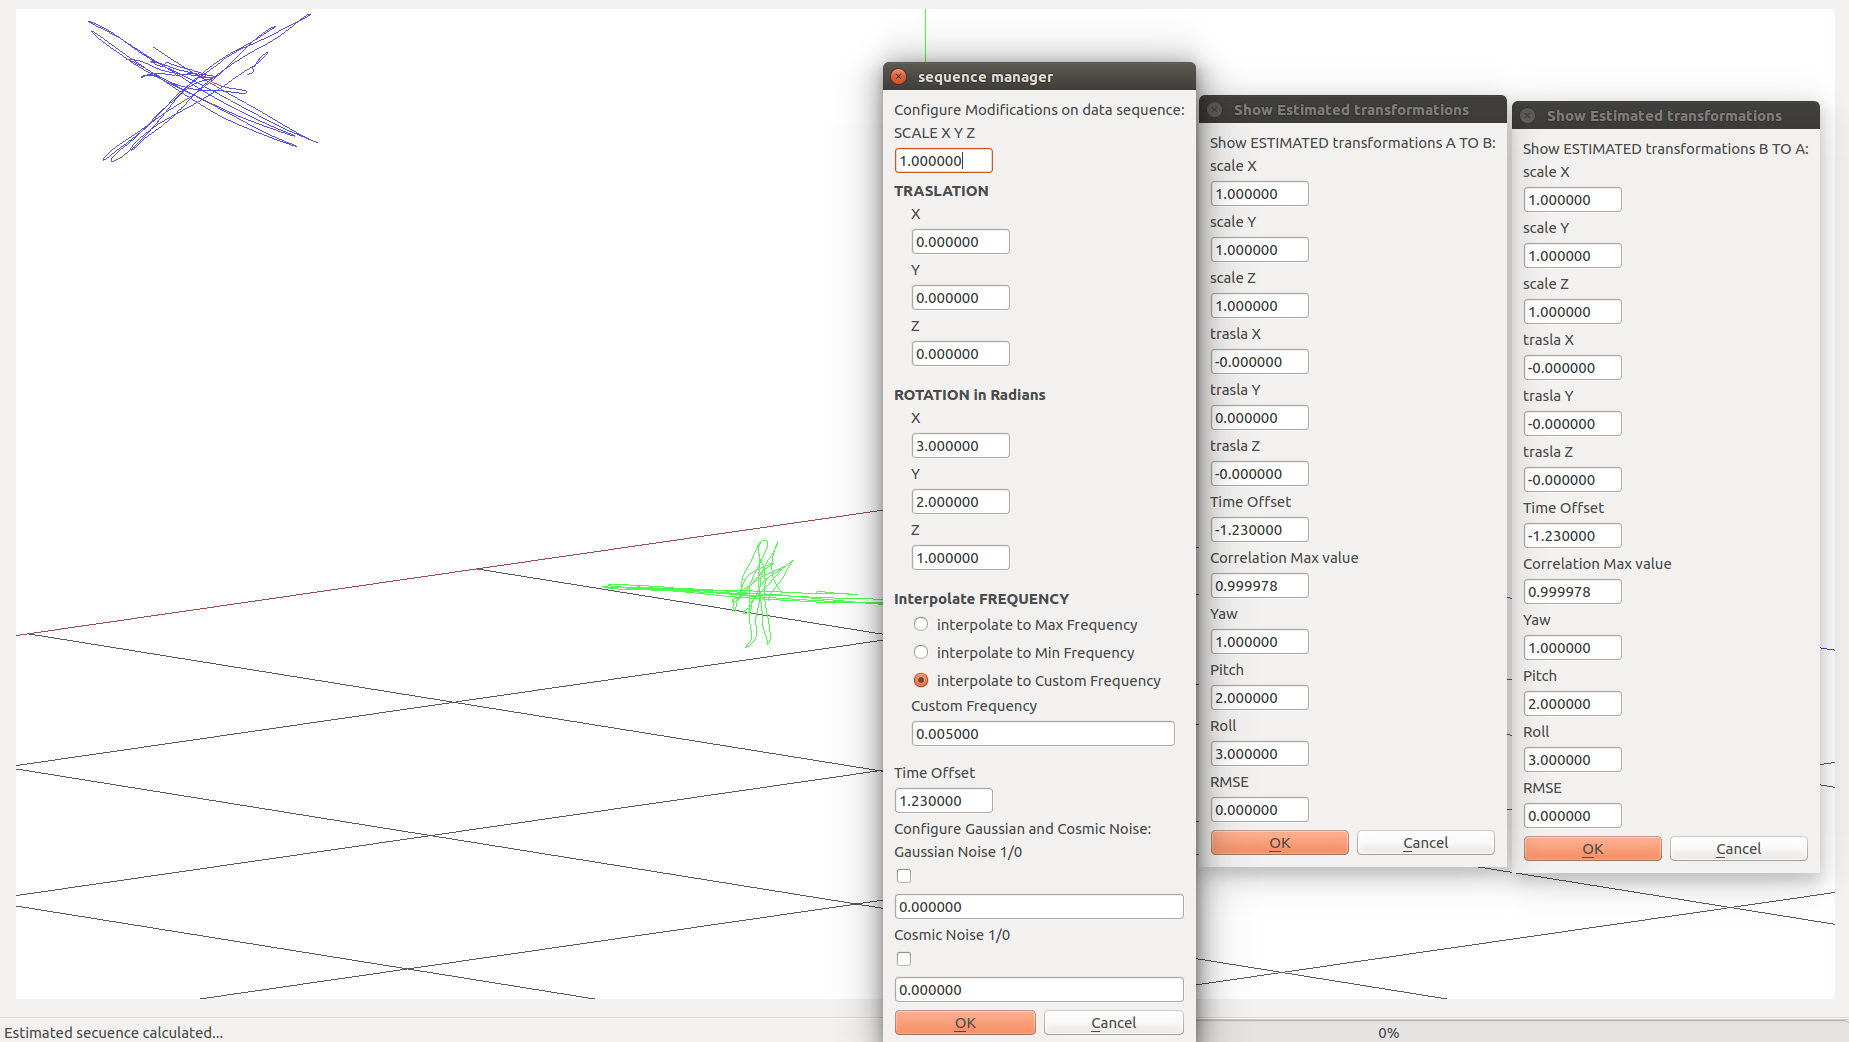
\includegraphics[height=14.0cm,width=18.0cm]{img/cap6/Rota_Offset_abba.png}
\hspace{0.5cm}

\end{center}

\caption{Resultados de la estimación de un cambio de rotación y offset.}
\end{figure}

En la Figura 5.13 al dataset original (color verde) se le ha aplicado un par de transformaciones (en rotación y con offset temporal), dando lugar al dataset transformado (conjunto de puntos de color azul). También la estimación es buena, ya que el error RMSE da como resultado 0.0 y el cálculo del offset coincide con el valor del offset que se ha aplicado en la transformación, salvo con signo negativo.


\subsection{Pruebas con rotación y ruido gaussiano}
\begin{figure}[H]
\begin{center}
\label{fig:opciones de View}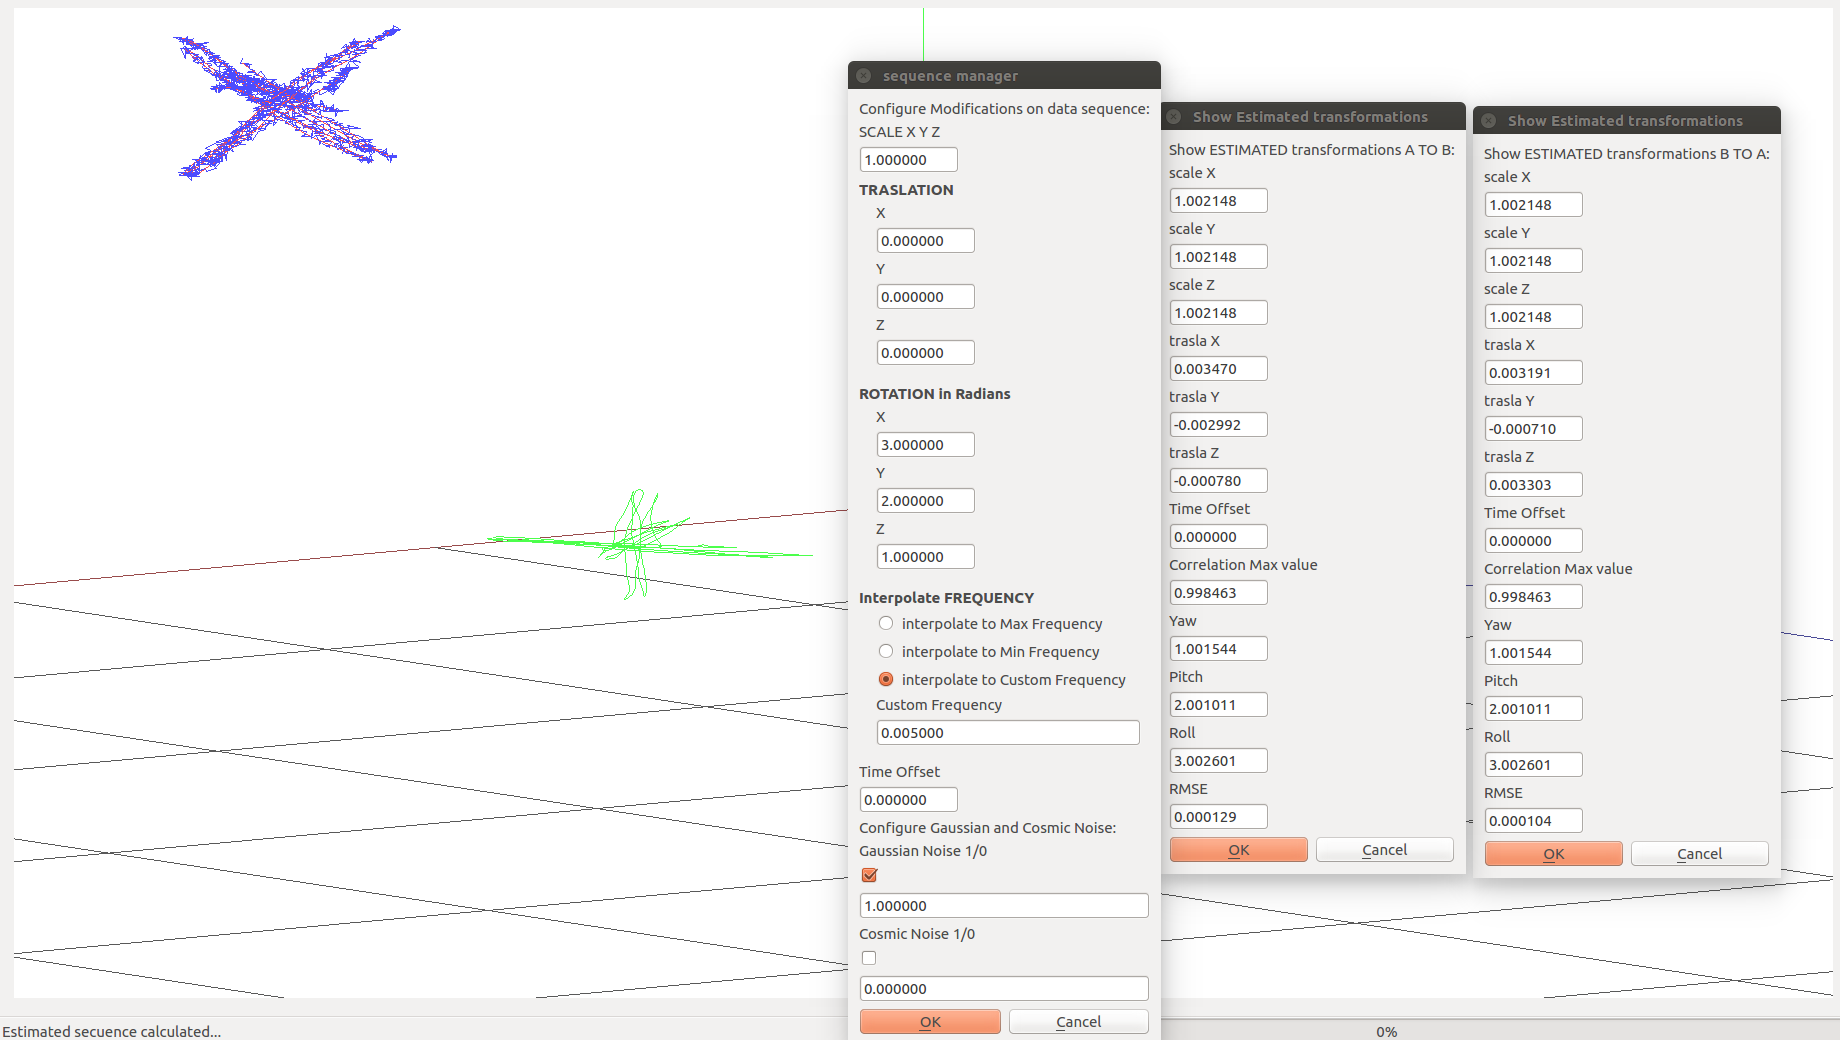
\includegraphics[height=14.0cm,width=18.0cm]{img/cap6/Rota_GaussNoise_abba.png}
\hspace{0.5cm}

\end{center}

\caption{Resultados de la estimación de un cambio de rotación y ruido gaussiano.}
\end{figure}
En la Figura 5.14 se ha aplicado sobre el dataset original un cambio de rotación y además se le ha añadido ruido gaussiano, como puede verse en el dataset resultante (color azul). Las estimaciones obtenidas son buenas, pero el error RMSE calculado entre el dataset transformado y el dataset estimado ya no es 0.0, sino 0.000129. Esta falta de exactitud puede apreciarse a simple vista en el interfaz gráfico, ya que como el dataset estimado carece de ruido gaussiano, los puntos del dataset estimado no coinciden con los puntos del dataset transformado, y por tanto ahora si podemos ver buena parte de los puntos del dataset estimado (color rojo).


\subsection{Pruebas con rotación y ruidos gaussiano y cósmico}

\begin{figure}[H]
\begin{center}
\label{fig:opciones de View}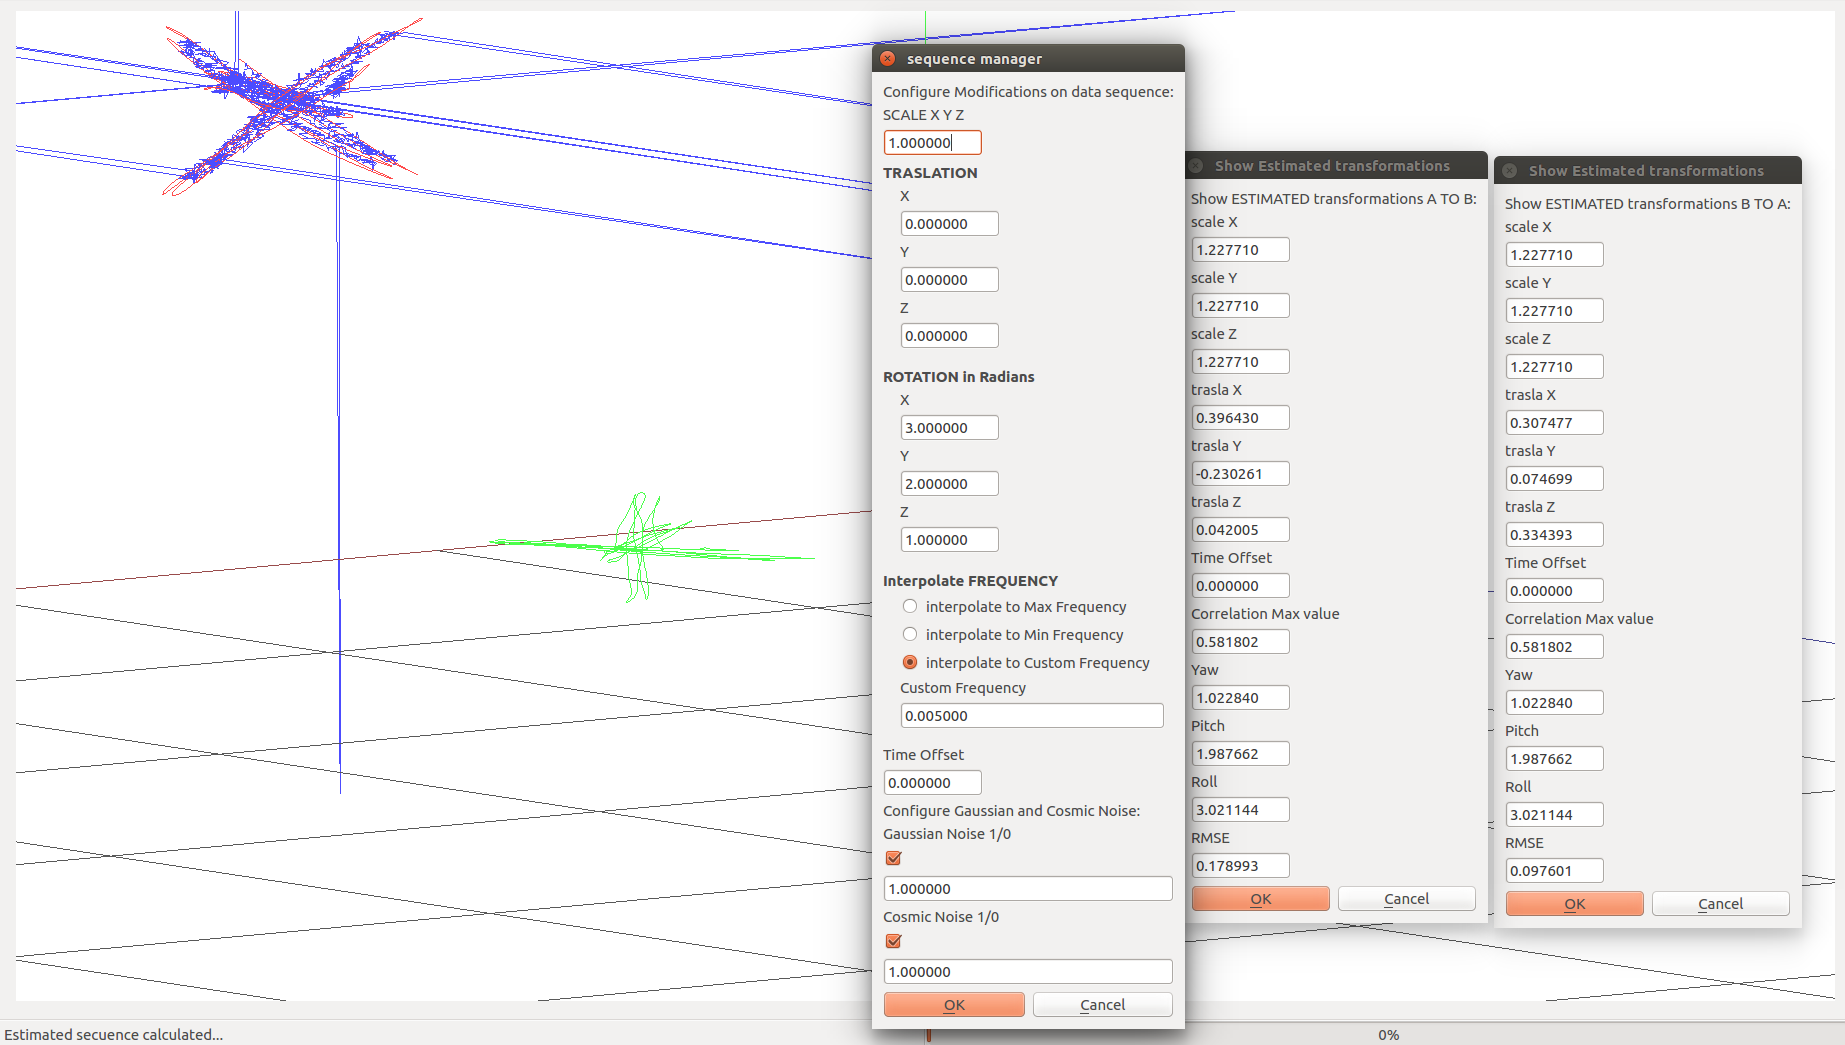
\includegraphics[height=14.0cm,width=18.0cm]{img/cap6/Rota_Gauss_Cosmic_abba.png}
\hspace{0.5cm}

\end{center}

\caption{Resultados de la estimación de un cambio de rotación y ruido cósmico y gaussiano.}
\end{figure}

En la Figura 5.15 se ha aplicado sobre el dataset original un cambio de rotación más ruido gaussiano y cósmico. Al tener ahora ruido cósmico, en algunos puntos del dataset transformado aparecen unos valores muy superiores al rango de valores del dataset, estos valores desorbitados hacen que aumente notablemente el error entre el dataset transformado y el dataset estimado. Para este experimento, el valor RMSE es de 0.17.  Puede observarse que aún así, la posición de los puntos del dataset estimado coincide con la posición de los puntos del dataset transformado.
También se observa como el ruido cósmico y gaussiano afectan a la estimación de otros parámetros, como escala y traslación, que en ausencia de ruido se estimaron con máxima exactitud y precisión como se puede ver en la Figura 5.13


%\newpage
\section{Validación experimental aplicando múltiples transformaciones simultáneas}

En este apartado mostraremos imágenes del módulo GUI, en las que se han realizado varias pruebas de transformaciones combinadas y se han estimado con SLAMTestbed dichas transformaciones entre secuencias.
En todas ellas se ha realizado la interpolación de frecuencias al valor 0.005 para ambos datasets.

Estos experimentos son los más exigentes para SLAMTestbed ya que ponen a prueba sus estimaciones cuando la relación entre las dos secuencias de entrada es compleja, combina varias transformaciones simultáneamente. Sin embargo son los experimentos más fiables porque son los que más se parecen al uso real de SLAMTestbed evaluando un nuevo algoritmo de VisualSLAM. La relación entre las estimaciones de ese algoritmo y las posiciones y estimaciones verdaderas será típicamente compleja e incluirá muchos ruidos y transformaciones.

Las siguientes grupos de transformaciones serán aplicadas:
\begin{itemize}
	\item{Escala, Traslación y Rotación}
	\item{Escala, Traslación, Rotación y Offset Temporal}
	\item{Escala, Traslación, Rotación, Offset Temporal y Ruido Gaussiano}
	\item{Escala, Traslación, Rotación, Offset Temporal y Ruido Cósmico}
\end{itemize}

\subsection{Pruebas con cambio de escala, rotación y traslación}
\begin{figure}[H]
\begin{center}
\label{fig:opciones de View}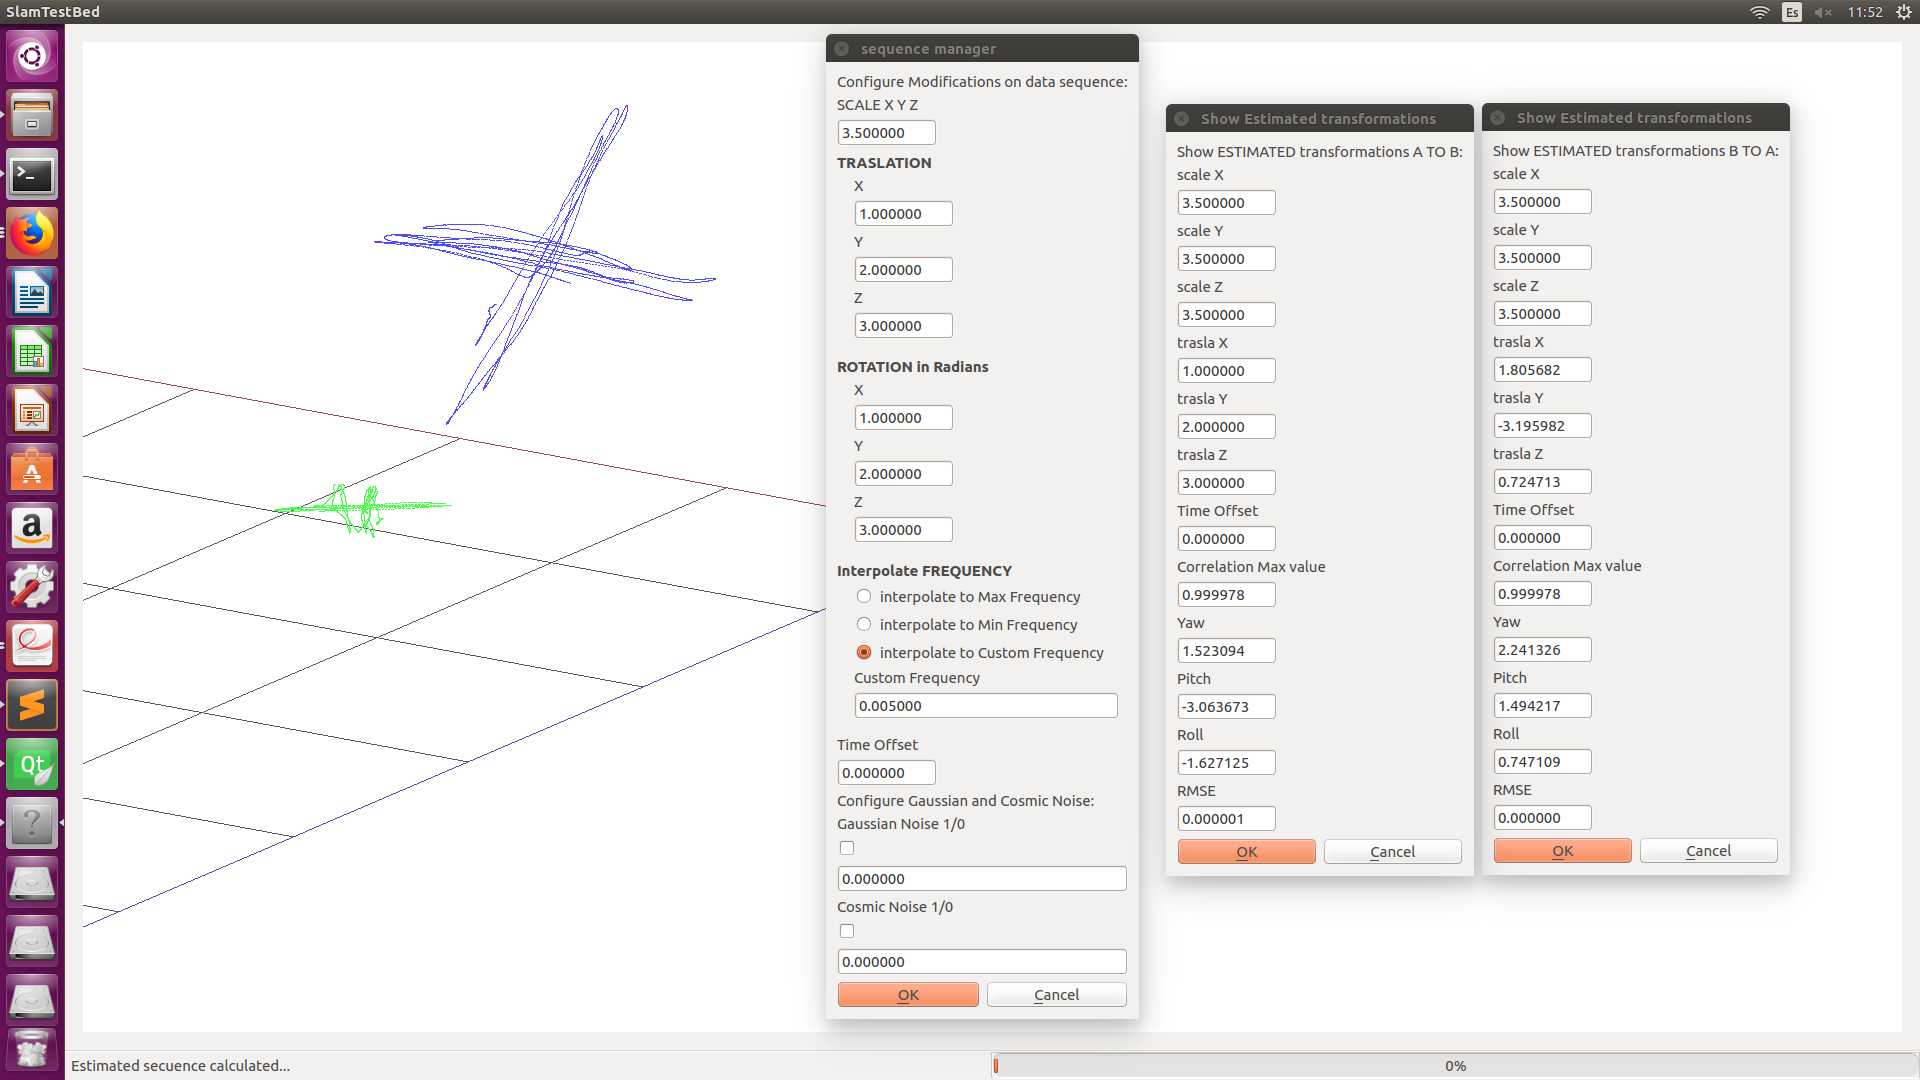
\includegraphics[height=14.0cm,width=18.0cm]{img/cap6/Escala_Trasla_Rota_abba.png}
\hspace{0.5cm}

\end{center}

\caption{Resultados de la estimación de un cambio de escala, traslación y rotación.}
\end{figure}

En la Figura 5.16 se realiza la estimación de las transformaciones que relacionan el dataset A al dataset B. En este caso se ha aplicado una transformación combinada de Escala, Traslación y Rotación. En verde puede verse el dataset original y en azul el dataset transformado, en rojo se aprecia el dataset estimado.
Se puede ver gráficamente cómo el dataset estimado se ajusta con gran precisión al dataset transformado (azul).
Por otra parte el RMSE entre el dataset transformado y el dataset estimado es de 0.000001
. Además las transformaciones se han calculado en los 2 sentidos, desde el dataset A  al dataset B y desde el dataset B al dataset A y coinciden.

\subsection{Pruebas con rotación, traslación, escala y offset temporal simultáneos.}
\begin{figure}[H]
\begin{center}
\label{fig:opciones de View}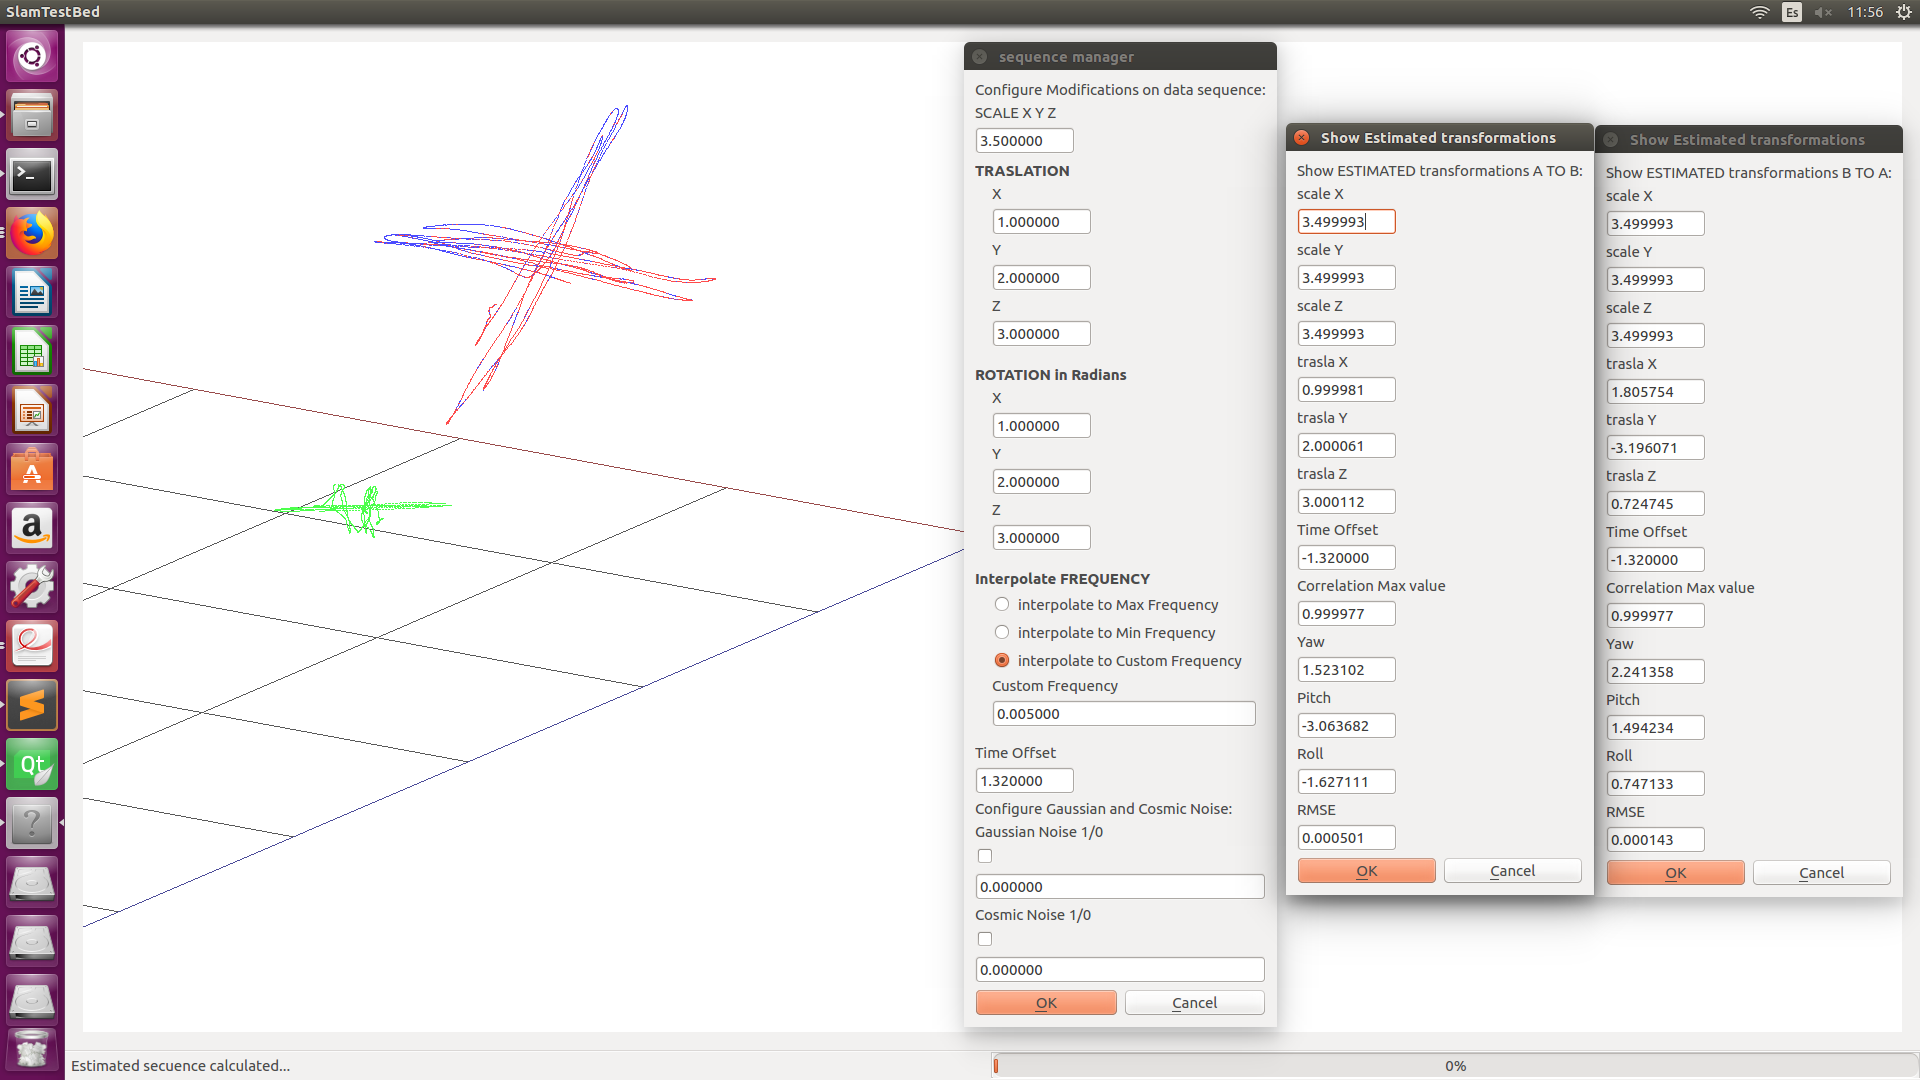
\includegraphics[height=14.0cm,width=18.0cm]{img/cap6/Escala_Trasla_Rota_Offset_abba.png}
\hspace{0.5cm}

\end{center}

\caption{Resultados de la estimación de un cambio de escala, traslación, rotación y offset simultáneos}
\end{figure}

En la Figura 5.17 se presenta el dataset original en verde, el dataset transformado en azul y el dataset estimado en rojo.
En este caso se ha realizado la combinación de transformaciones de Escala, Traslación, Rotación y Offset.
Como se puede observar en los resultados de las estimaciones, el offset es estimado con total exactitud. Sin embargo el valor del RMSE ya no es exactamente 0.0, si no de 0.0005, aún así el error cometido sigue siendo muy bajo.
Visualmente, también se puede observar que la precisión ha disminuido, ya que se aprecian más puntos rojos (dataset estimado) en el gráfico. Esto indica que la estimación sigue siendo muy buena aunque la precisión ha bajado.



\subsection{Pruebas con traslación, rotación, escala, offset temporal y ruido gaussiano}
\begin{figure}[H]
\begin{center}
\label{fig:opciones de View}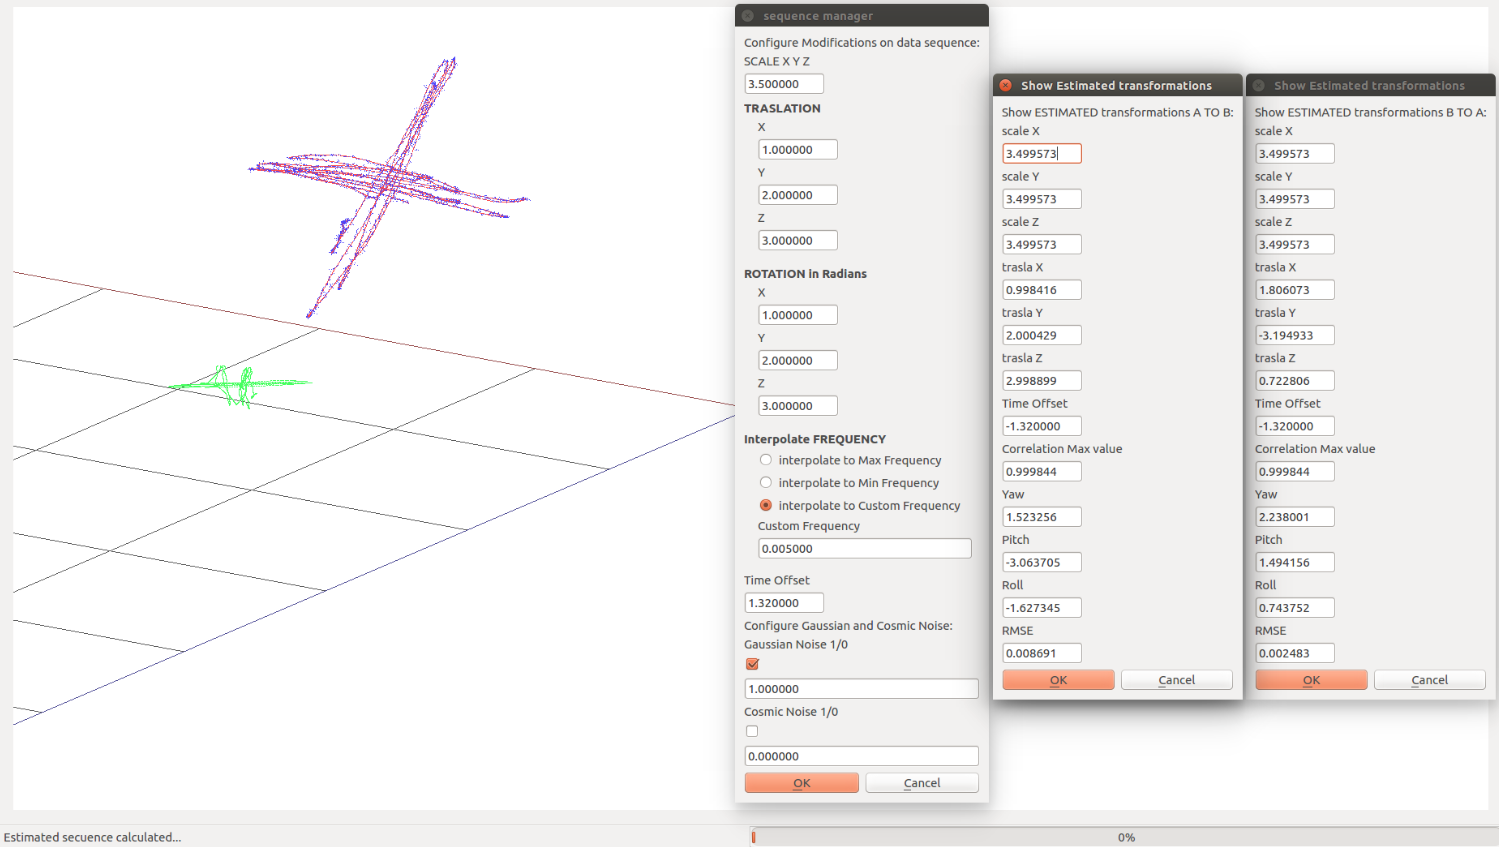
\includegraphics[height=14.0cm,width=18.0cm]{img/cap6/Escala_Trasla_Rota_Offset_GaussNoise_abba.png}
\hspace{0.5cm}

\end{center}

\caption{Resultados de la estimación de un cambio de escala y traslación, rotación, offset y ruido gaussiano simultáneos.}
\end{figure}
En la Figura 5.18, podemos ver el dataset original en verde, el dataset transformado en azul y el dataset estimado en rojo.
Las transformaciones realizadas en este caso han sido, Escala, Traslación, Rotación, Offset y Ruido Gaussiano.
En este caso, al incluir ruido gaussiano en la transformación del dataset original, el dataset estimado pierde algo de precisión, y el RMSE obtenido es de  0.008.
Sin embargo, la precisión aunque es menor, continúa siendo buena, y en el gráfico puede verse cómo el dataset estimado concuerda de manera aceptable con el dataset transformado. Obsérvese que en el dataset estimado no hay ruido gaussiano.
\subsection{Pruebas completas con traslación, rotación, escala, offset temporal, ruido gaussiano y cósmico}
\begin{figure}[H]
\begin{center}
\label{fig:opciones de View}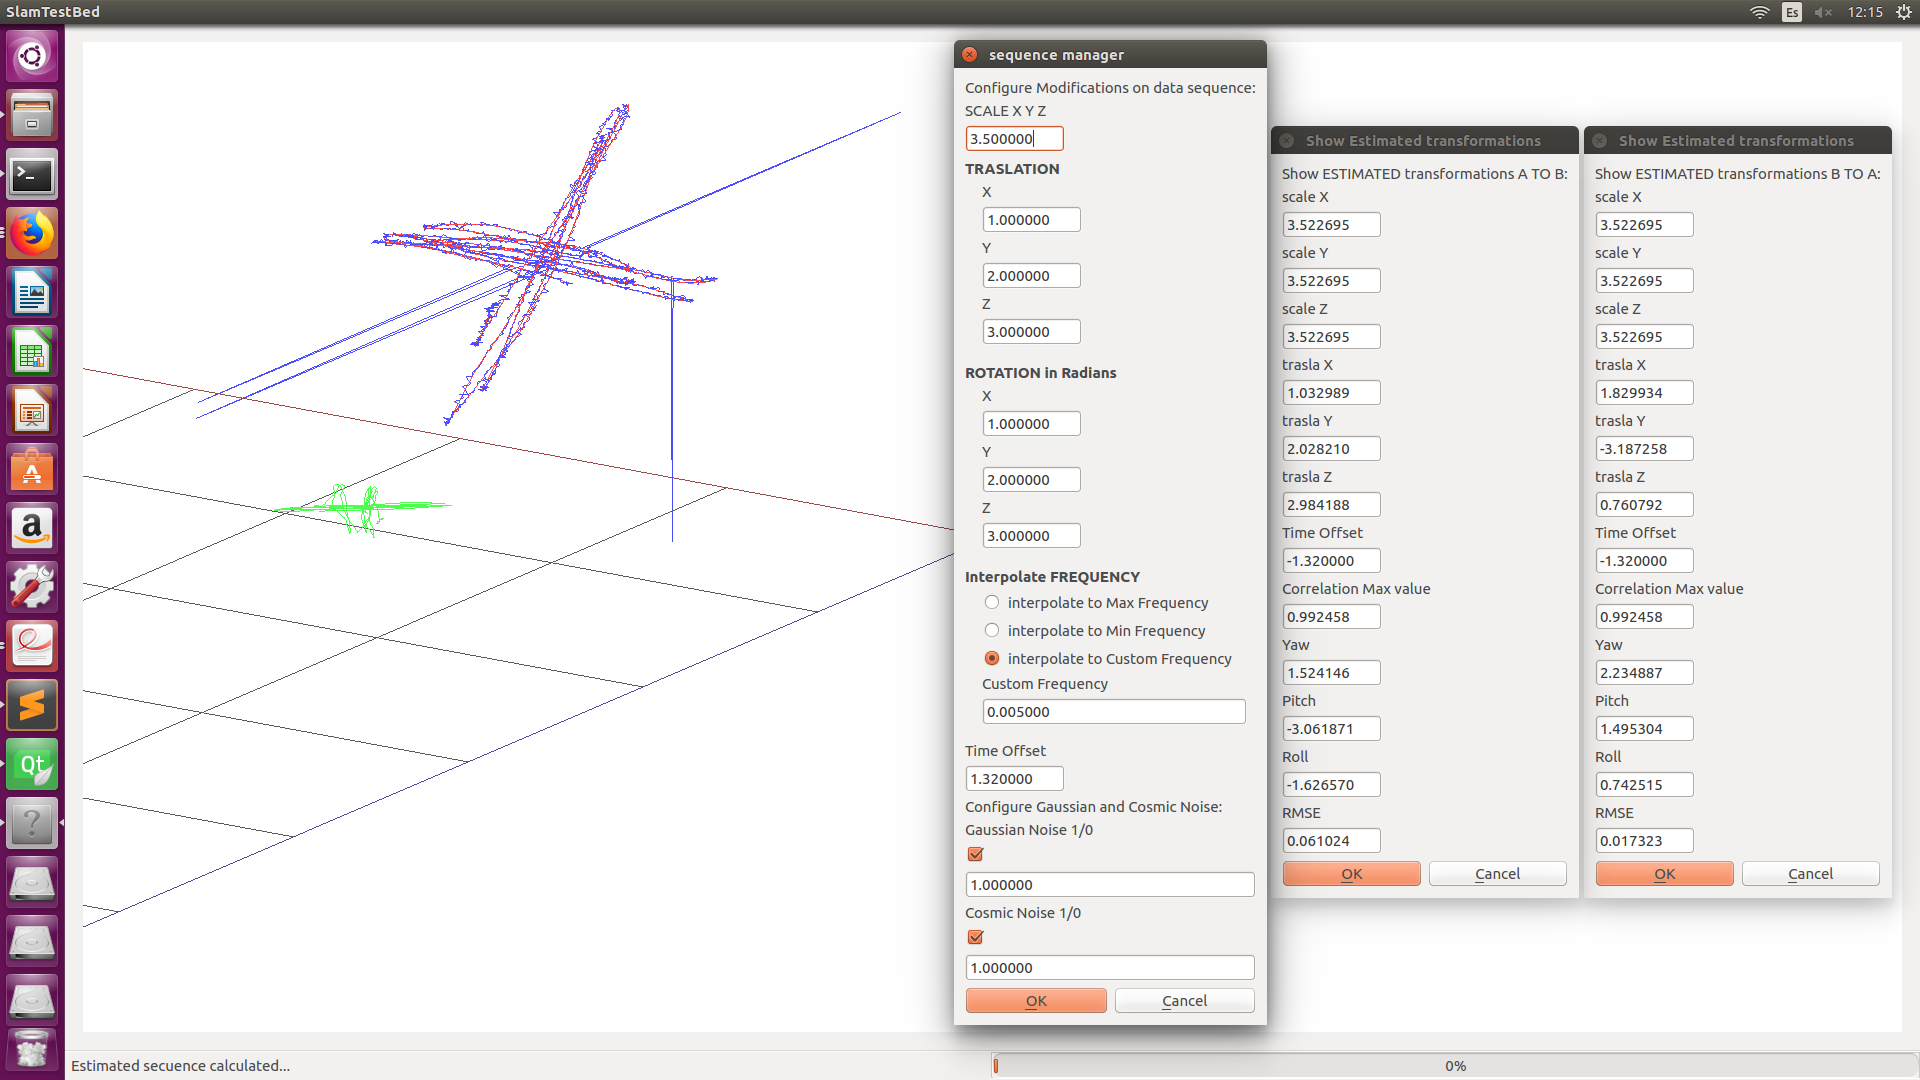
\includegraphics[height=14.0cm,width=18.0cm]{img/cap6/Escala_Trasla_Rota_Offset_Gauss_CosmicNoise_abba.png}
\hspace{0.5cm}
\end{center}
\caption{Resultados de la estimación de un cambio de escala y traslación, rotación, offset temporal, ruidos gaussiano y cósmico.}
\end{figure}
En la imagen 5.19 podemos ver una nueva captura de pantalla, donde se han realizado las siguientes transformaciones: Escala, Traslación, Rotación, Offset, Ruido Gaussiano y Ruido Cósmico.
Como se puede observar, en las estimaciones del dataset A ( verde ) al dataset B (azul), la precisión ha bajado notablemente, con un valor RMSE del 0.06.
Esta precisión tan baja se debe a la inclusión de ruido cósmico, que altera notablemente los valores de X, Y , Z  de algunos puntos 3D.
Aún así, como puede verse en  la representación gráfica del dataset Estimado (rojo) sobre el dataset Transformado ( azul ) se aproxima bastante a la solución perfecta.

\subsection{Pruebas completas con traslación, rotación, escala, offset temporal, ruido gaussiano, ruido cósmico y RANSAC}


%\begin{figure}[H]
%\begin{center}
%\label{fig:opciones de View}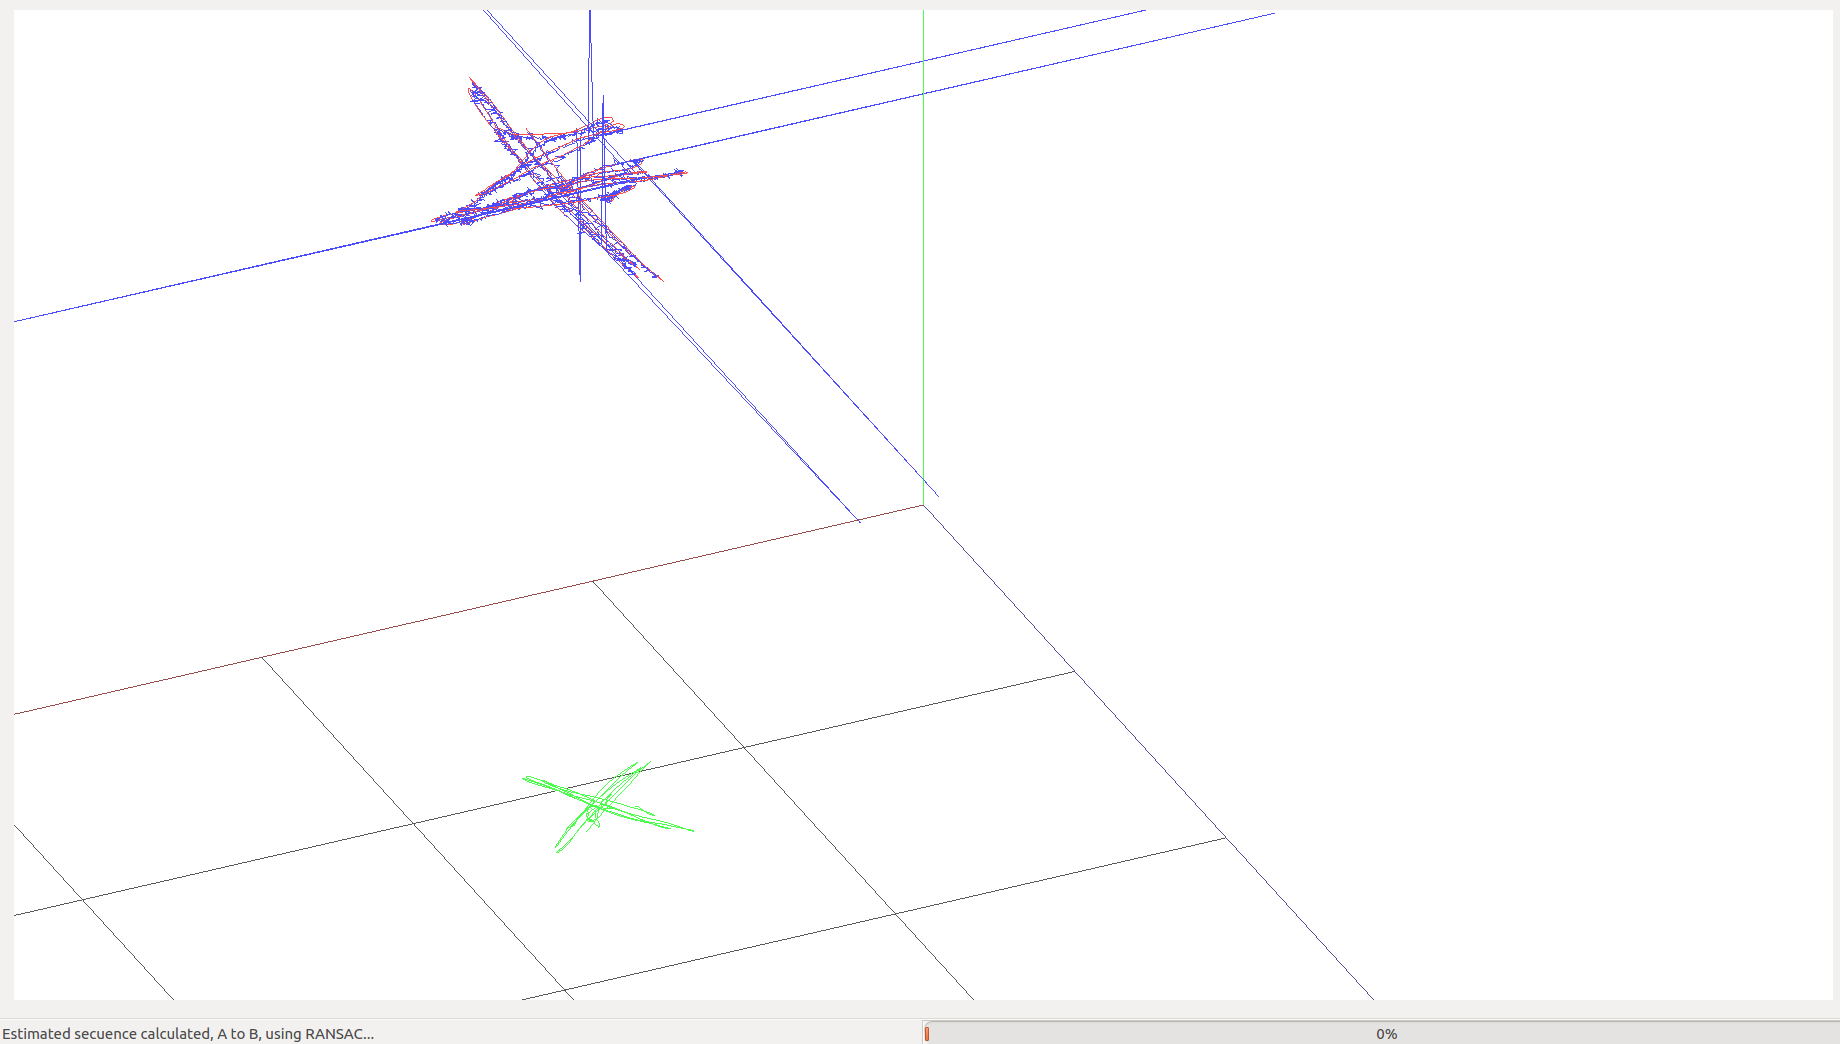
\includegraphics[height=14.0cm,width=18.0cm]{img/cap6/SalaTraslaRotaGausCosmicNoise-ab.png}
%\hspace{0.5cm}

%\end{center}

%\caption{Resultados de la estimación  utilizando RANSAC.}
%\end{figure}

%En la Figura 5.20, 
%En este caso mostraremos la diferencia entre estimar los resultados aplicando los %algoritmos normales o aplicando RANSAC. En esta figura el dataset estimado se aproxima al groundtrouth, pero no coincide exactamente, de ahí que sea tan visible (en rojo) el dataset estimado.


\begin{figure}[H]
\begin{center}
\label{fig:opciones de View}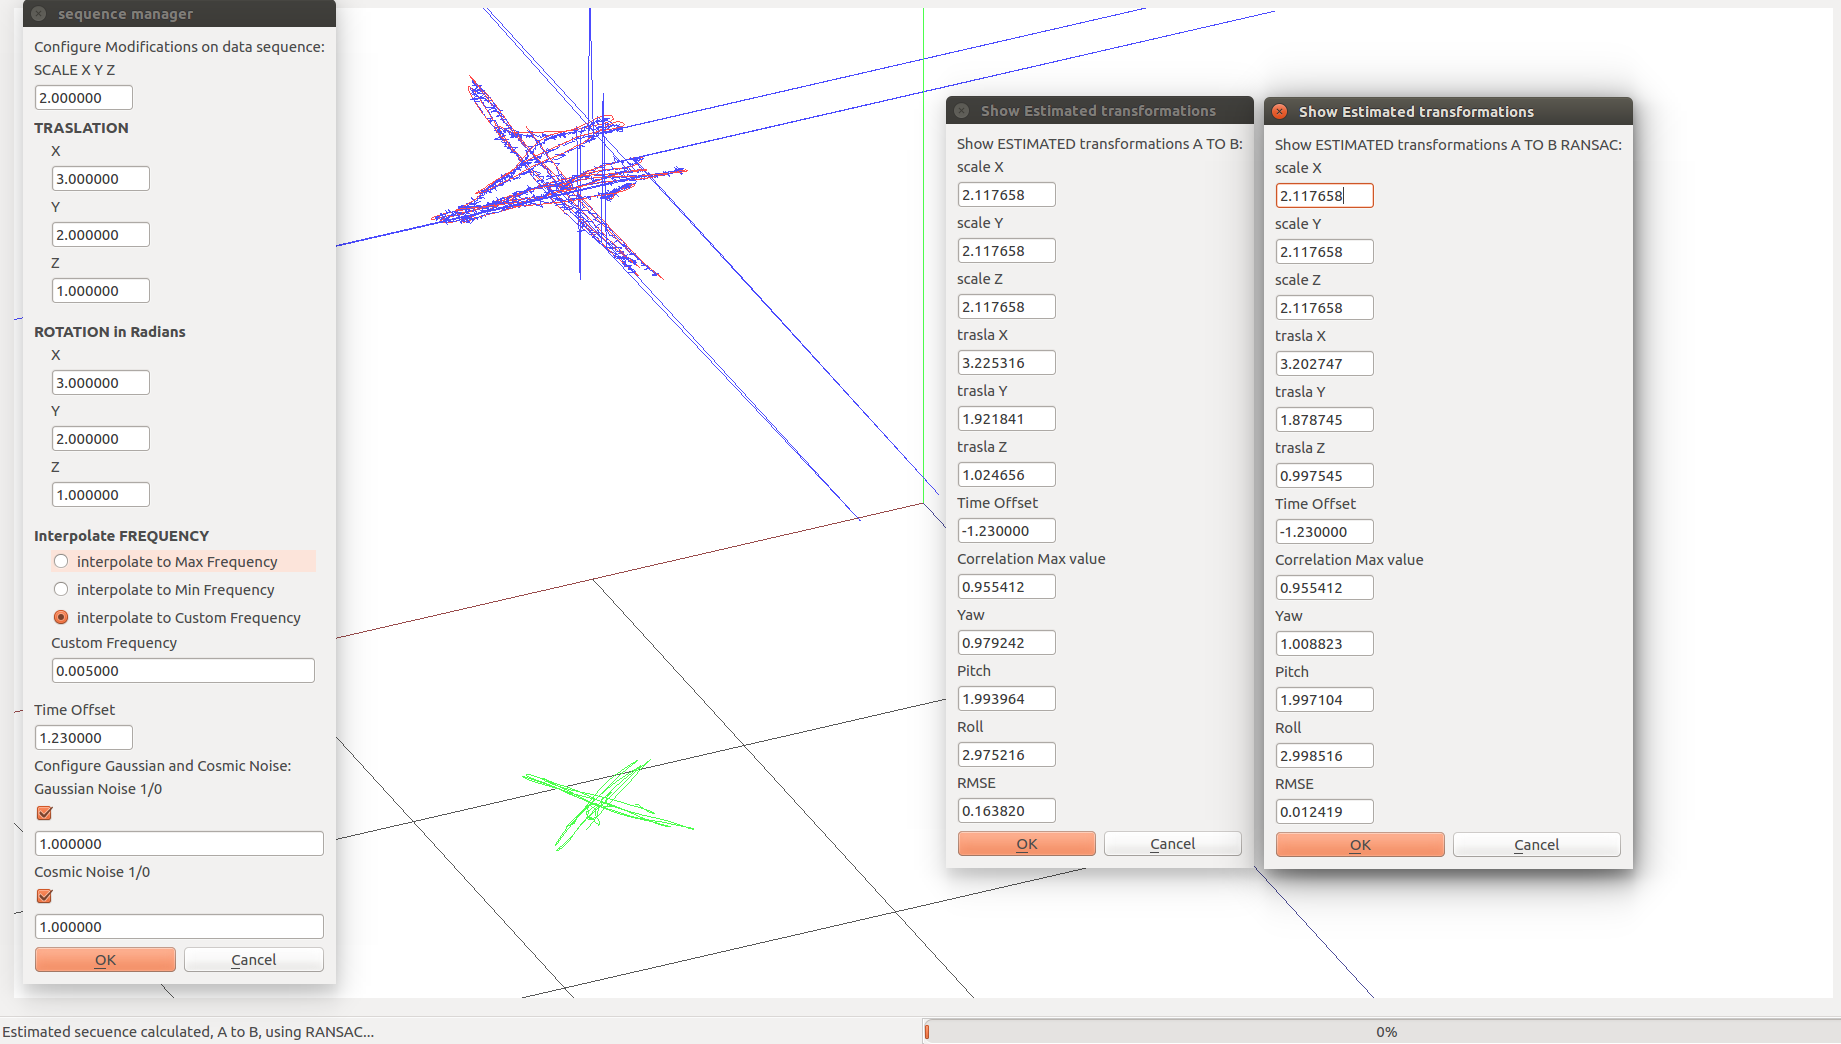
\includegraphics[height=14.0cm,width=18.0cm]{img/cap6/RANSAC_ScaleTraslaRotaGausCosmicNoise_ab.png}
\hspace{0.5cm}

\end{center}

\caption{Resultados de la estimación  utilizando RANSAC.}
\end{figure}

En la Figura 5.20 podremos ver una nueva transformación donde se ha aplicado transformaciones de Escala, Traslación, Rotación, Offset, Ruido Gaussiano y Cósmico. Mostramos los resultados de las estimaciones calculadas que relacionan el dataset A con el dataset B y comparamos con las estimaciones calculadas con RANSAC, observamos que el valor obtenido del RMSE en el caso de RANSAC (0,012) es menor que en el caso de no aplicar RANSAC (0,16), por tanto se consigue una estimación más precisa cuando aplicamos RANSAC.

Otra variación la encontramos en la Escala, para el cálculo de la escala no se ha utilizado RANSAC en ningún caso, de aquí que los valores obtenidos en ambos casos sean similares y presenten un cierto error con el \textit{groundtrouth}, (2.117 frente al valor real de 2.0). 

En SLAMTestbed, el algoritmo de RANSAC sólo se ha implementado como opción para la estimación de la matriz de Rotación y Traslación.
La utilización de RANSAC para el cálculo de la Escala quedaría como futura mejora de la herramienta SLAMTestbed.


\newpage

\subsection {Pruebas de transformaciones combinadas usando trayectoria de un dataset internacional}

En las siguientes pruebas seguimos comparando una secuencia pura con la secuencia obtenida tras aplicarle las transformaciones deseadas con el módulo transformador. Esta secuencia pura es otro caso real SLAM (en tamaño de momientos, amplitud de rotaciones, frecuencias de muestreo, etc.) y se ha tomado de un dataset internacional público. \footnote{\url{https://svncvpr.in.tum.de/cvpr-ros-pkg/trunk/rgbd_benchmark/rgbd_benchmark_tools/data/rgbdslam/}}

\begin{figure}[H]
\begin{center}
\label{fig:secondTrayectory}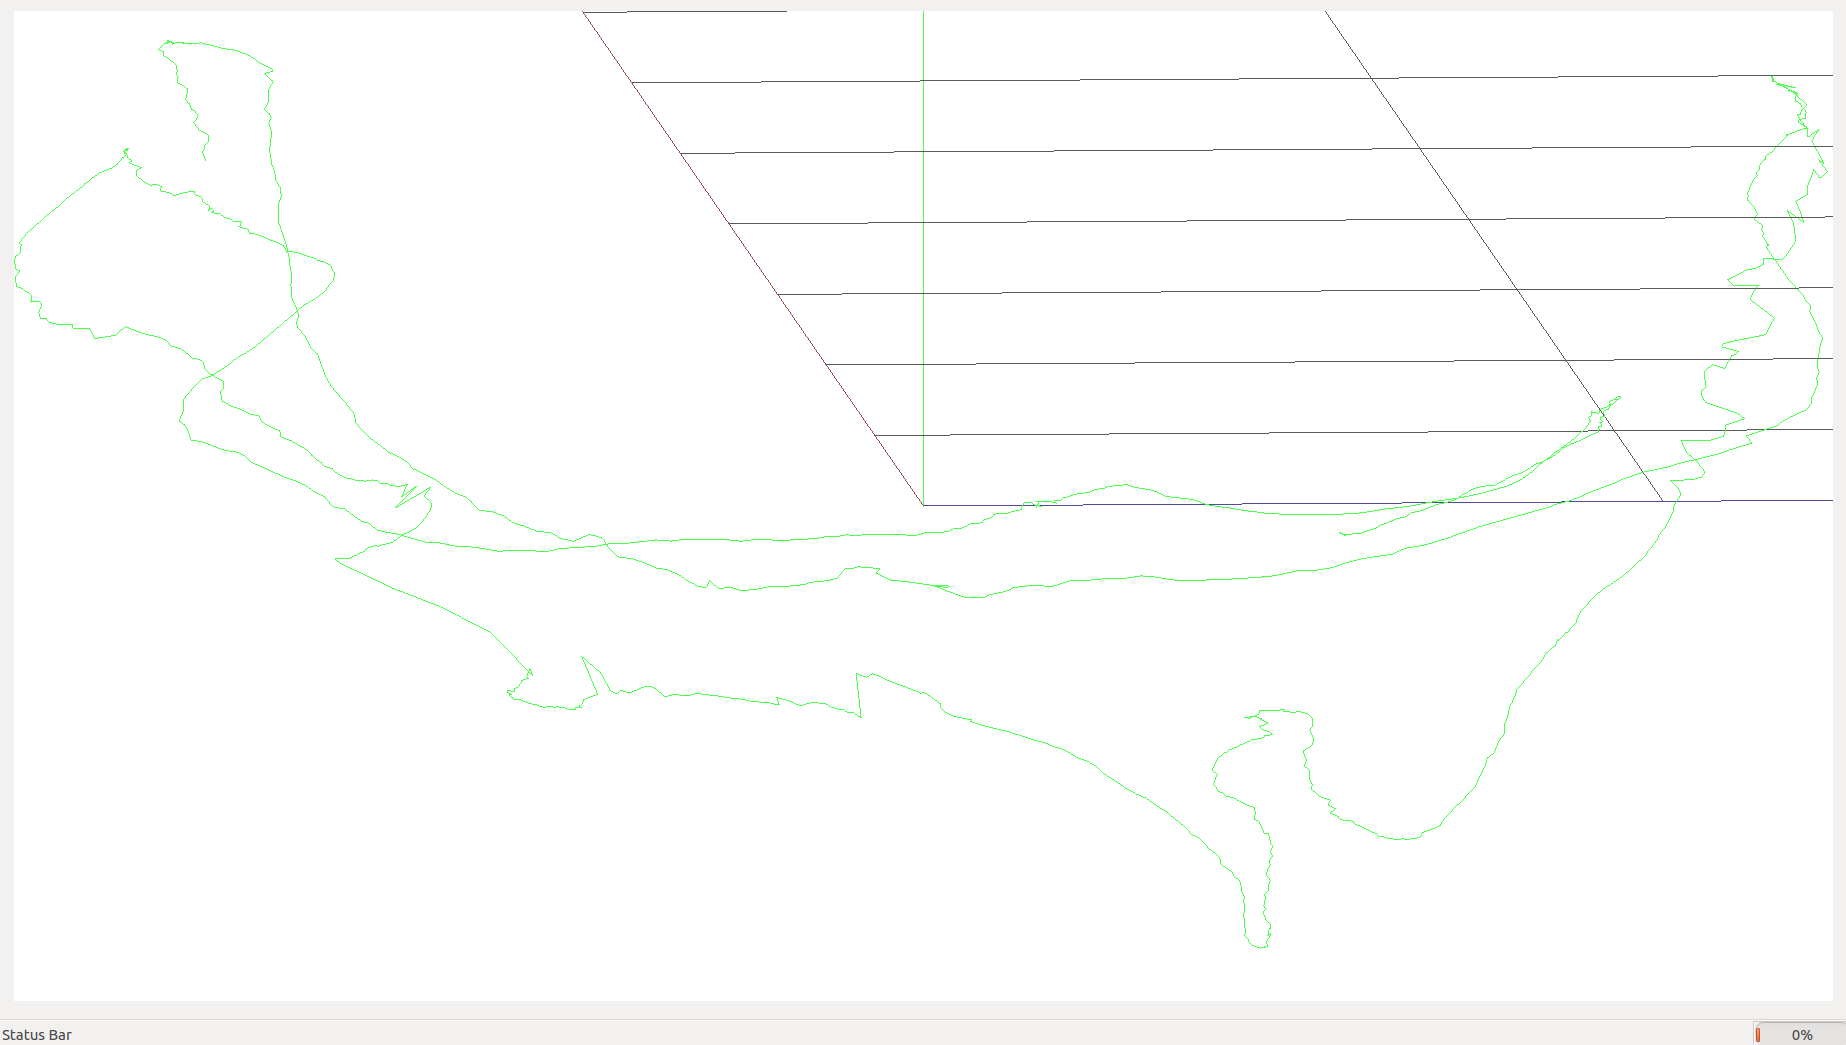
\includegraphics[height=14.0cm,width=18.0cm]{img/cap6/segundaTrayectoria.png}
\hspace{0.5cm}

\end{center}
\caption{ Segunda trayectoria visualizada en 3D y ampliada.}
\end{figure}

\begin{figure}[H]
\begin{center}
\label{fig:opciones de View}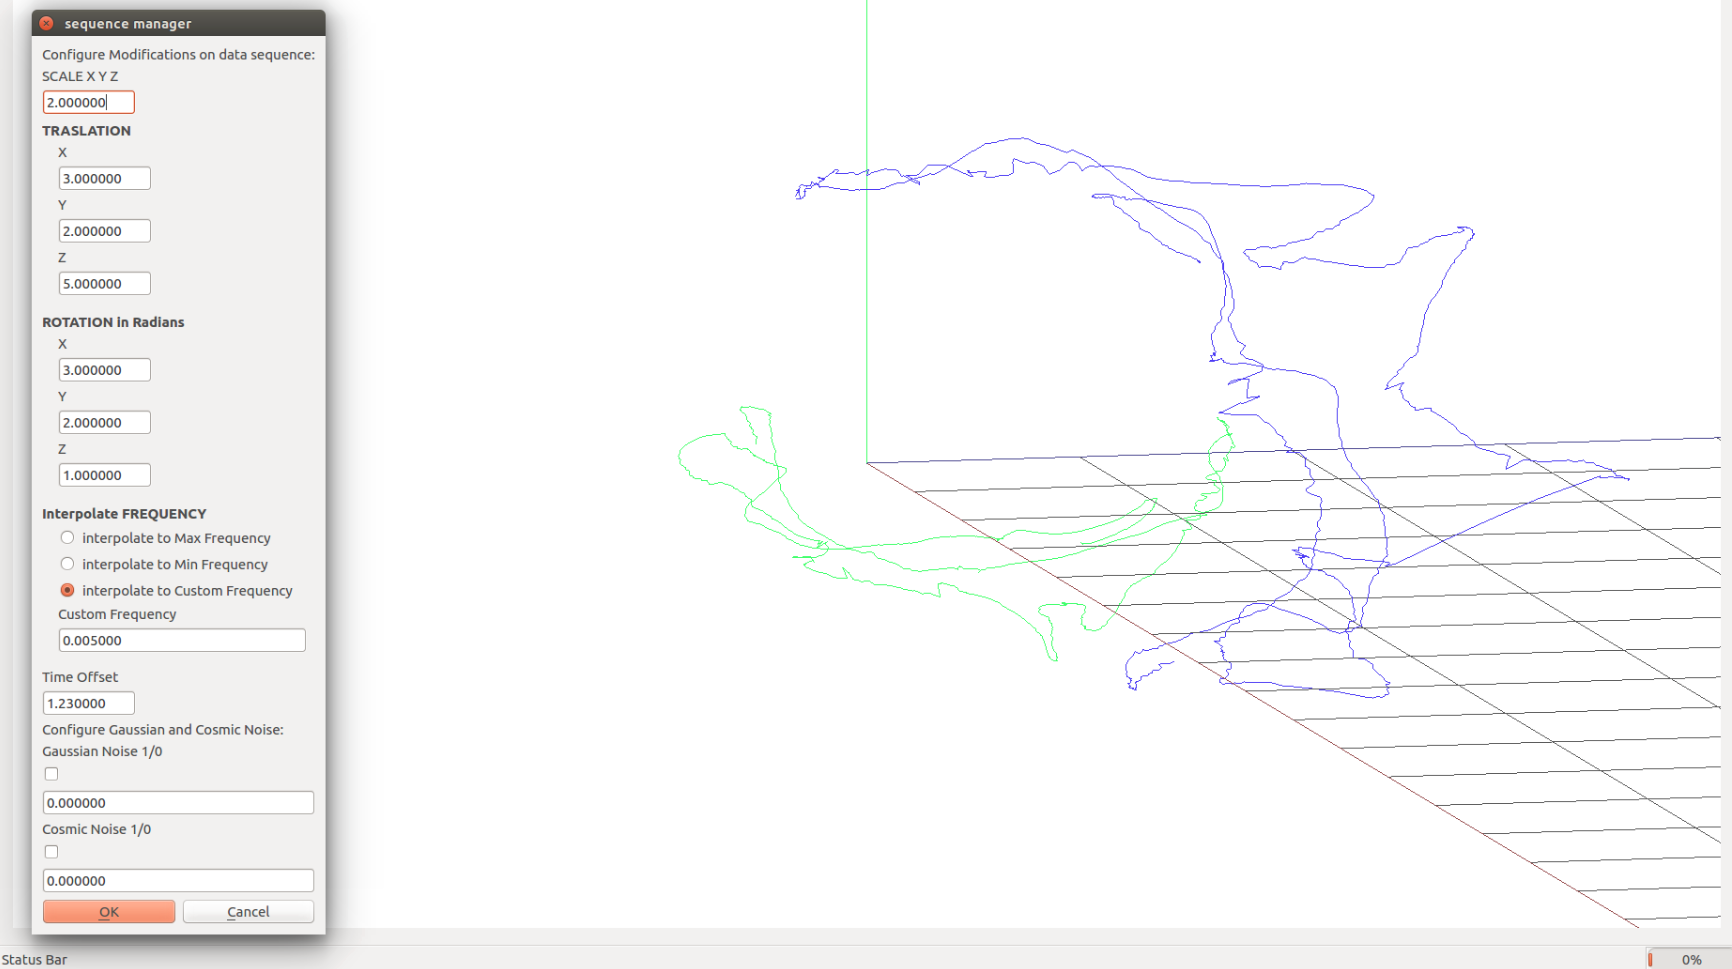
\includegraphics[height=14.0cm,width=18.0cm]{img/cap6/newData_Transformations.png}
\hspace{0.5cm}

\end{center}

\caption{ Configuración de transformaciones para la nueva secuencia.}
\end{figure}
La Figura 5.22, a la izquierda muestra la configuración de transformaciones para la nueva secuencia, donde inicialmente se aplicará una combinación de transformaciones de Escala, Traslación, Rotación y Offset temporal. A la derecha puede verse el dataset A (original) en verde, y el dataset B (transformado) en azul.

\begin{figure}[H]
\begin{center}
\label{fig:opciones de View}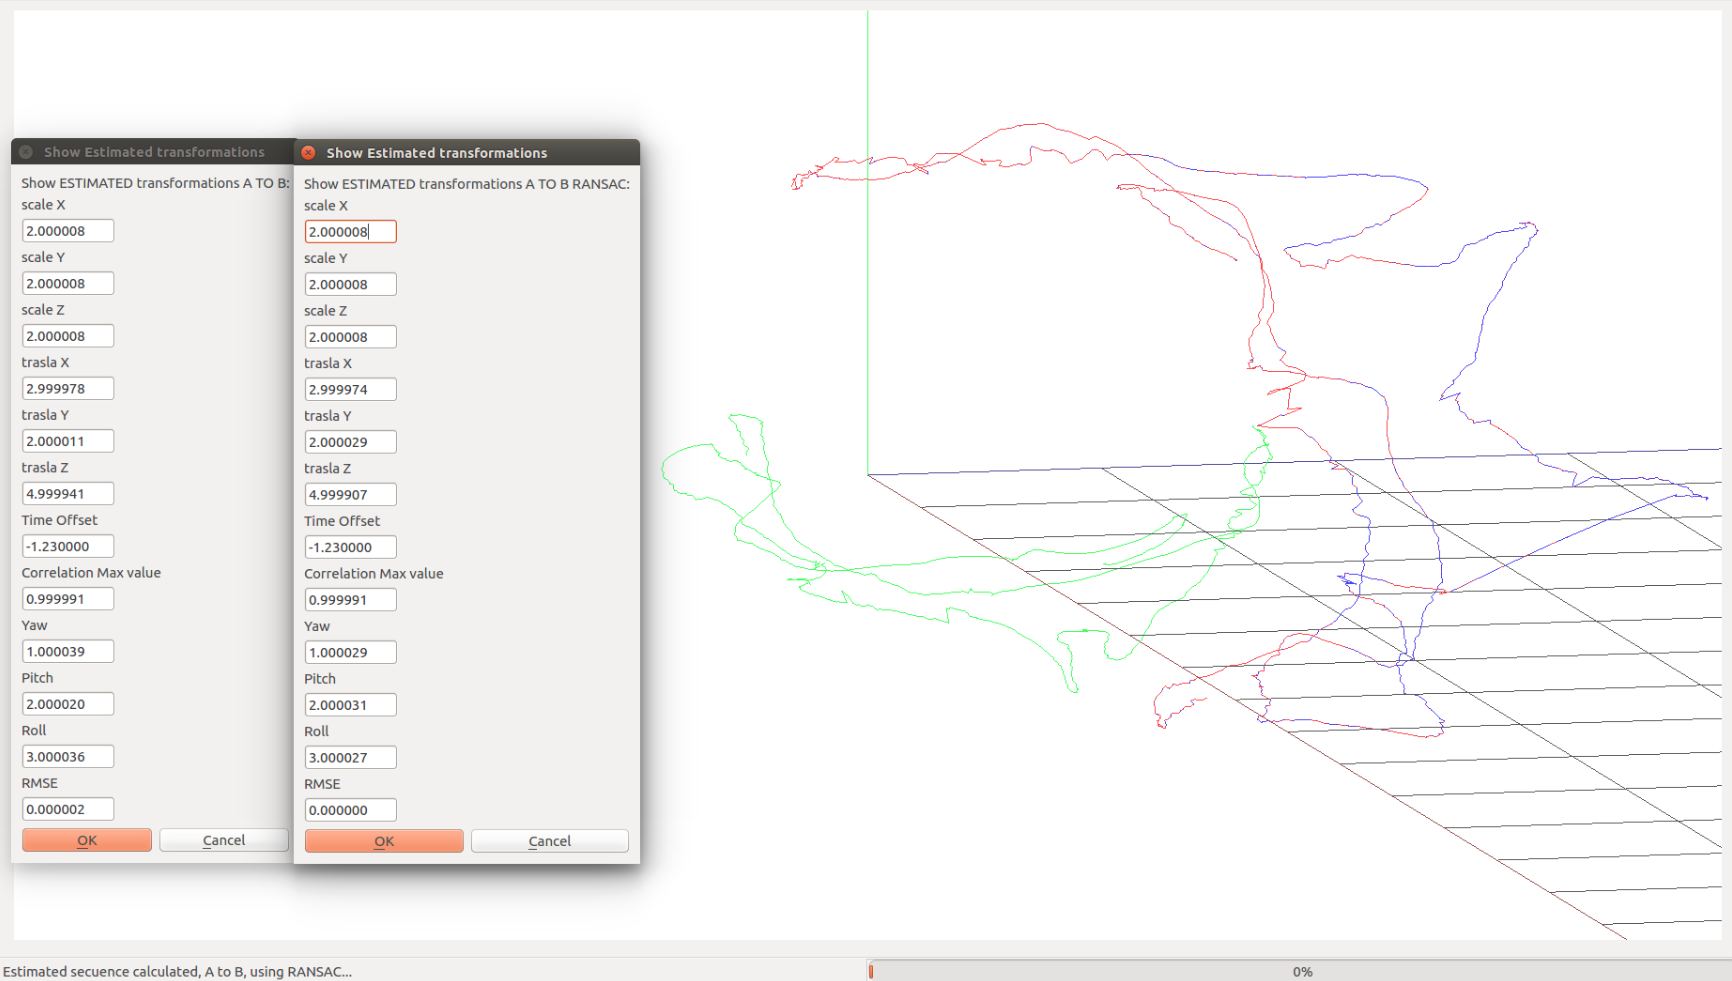
\includegraphics[height=14.0cm,width=18.0cm]{img/cap6/newData_EscalaTraslaRota_aB.png}
\hspace{0.5cm}

\end{center}

\caption{Resultados de las estimaciones A to B, sin RANSAC y con RANSAC.}
\end{figure}
En la Figura 5.23 pueden comprobarse los resultados de estimar las transformaciones entre el dataset A y el dataset B usando y sin usar RANSAC. 

A la izquierda podremos comprobar la diferencia entre aplicar RANSAC y no aplicarlo. Todos los parámetros estimados son muy aproximados a los originales salvo un ligero error. Obsérvese que en el caso de aplicar RANSAC el resultado del RMSE es 0, y el caso de no aplicar RANSAC el resultado es 0.000002.

En algunos tramos podemos ver el trazo rojo de la secuencia estimada pero no es visible el trazo azul de la secuencia transformada. Esto significa que las dos secuencias no coinciden exactamente en las 3 coordenadas X,Y,Z pero la diferencia es mínima. Con una diferencia mayor entre las 2 secuencias, veríamos los 2 trazos (rojo y azul) alineados.


\begin{figure}[H]
\begin{center}
\label{fig:opciones de View}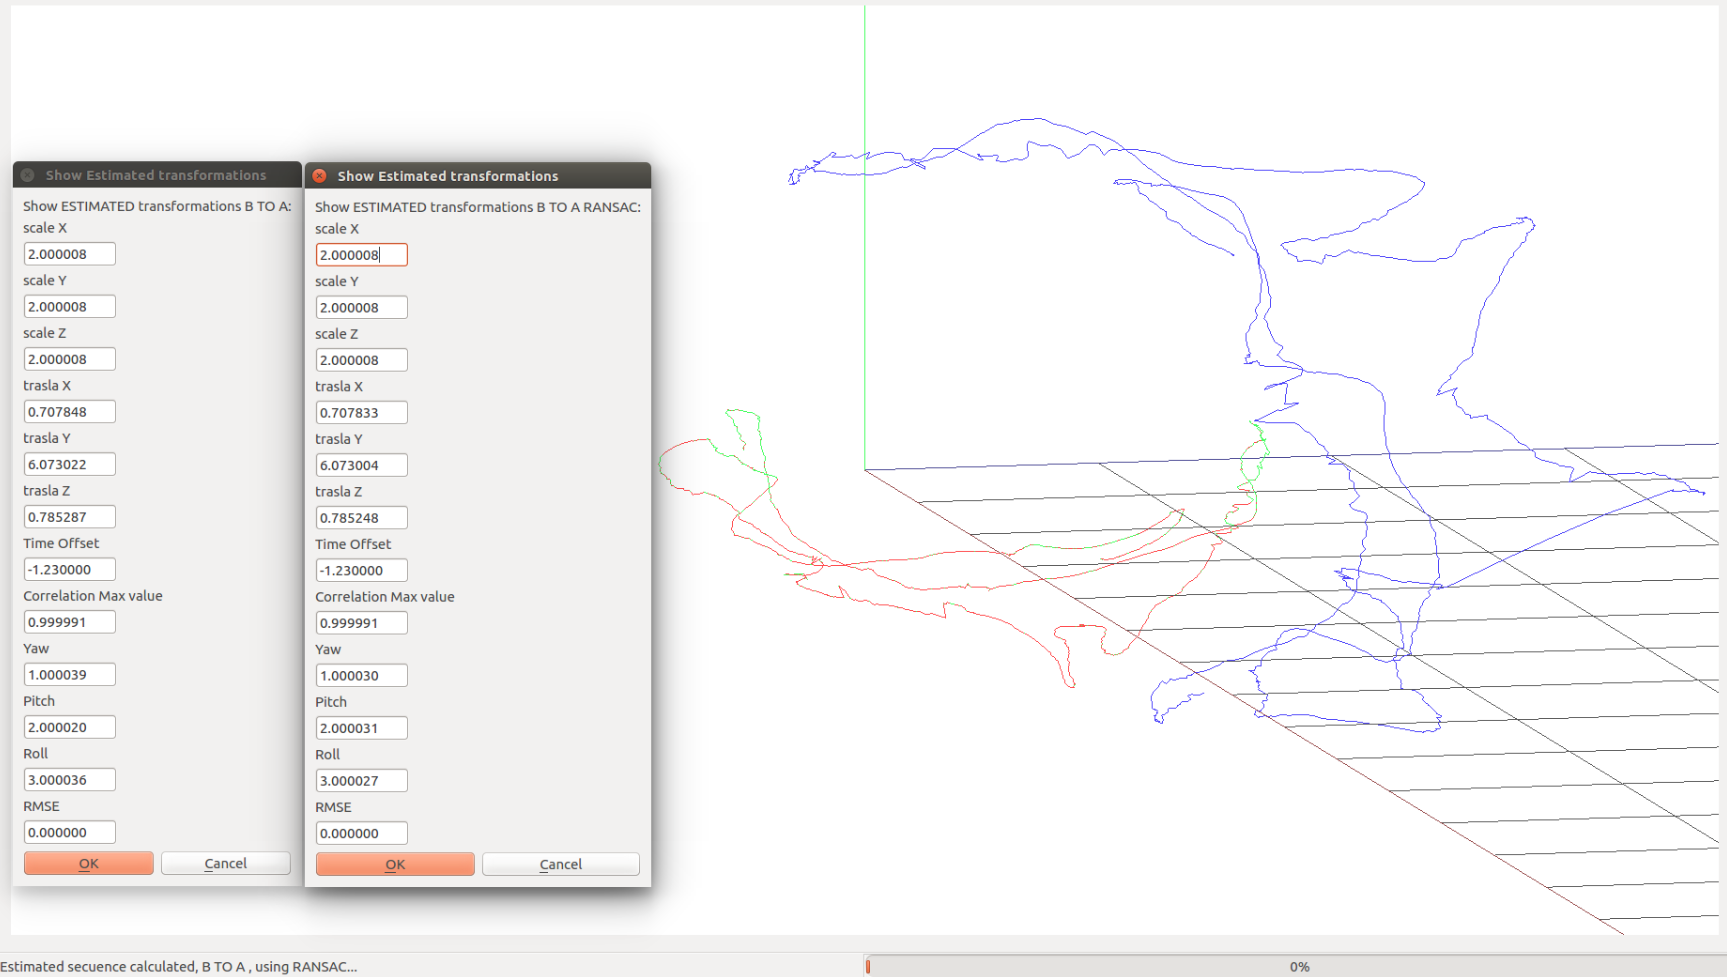
\includegraphics[height=14.0cm,width=18.0cm]{img/cap6/newData_EscalaTraslaRota_BA.png}
\hspace{0.5cm}

\end{center}

\caption{Resultados de las estimaciones B to A, sin RANSAC y con RANSAC.}
\end{figure}

En la Figura 5.24 puede observarse los resultados de estimar las transformaciones entre el dataset B y el dataset A, a la izquierda podemos comprobar numéricamente la diferencia entre aplicar RANSAC y no aplicarlo. Todos los parámetros son muy aproximados a los originales salvo un ligero error. En este caso, tanto aplicando RANSAC como sin él obtenemos un RMSE =  0. En el caso de los valores de la Traslación no se parecen a los originales, esto es debido a que se ha estimado una traslación equivalente a la transformación original de tal forma que el resultado de aplicar múltiples transformaciones coincide con los valores originales. Gráficamente podemos comprobar la exactitud de las transformaciones.

En algunos tramos podemos ver el trazo rojo de la secuencia estimada pero no es visible el trazo verde de la secuencia original. Esto significa que las dos secuencias no coinciden exactamente en las 3 coordenadas X,Y,Z pero la diferencia es mínima. Con una diferencia mayor entre las 2 secuencias, veríamos los 2 trazos (rojo y verde) alineados.

\begin{figure}[H]
\begin{center}
\label{fig:opciones de View}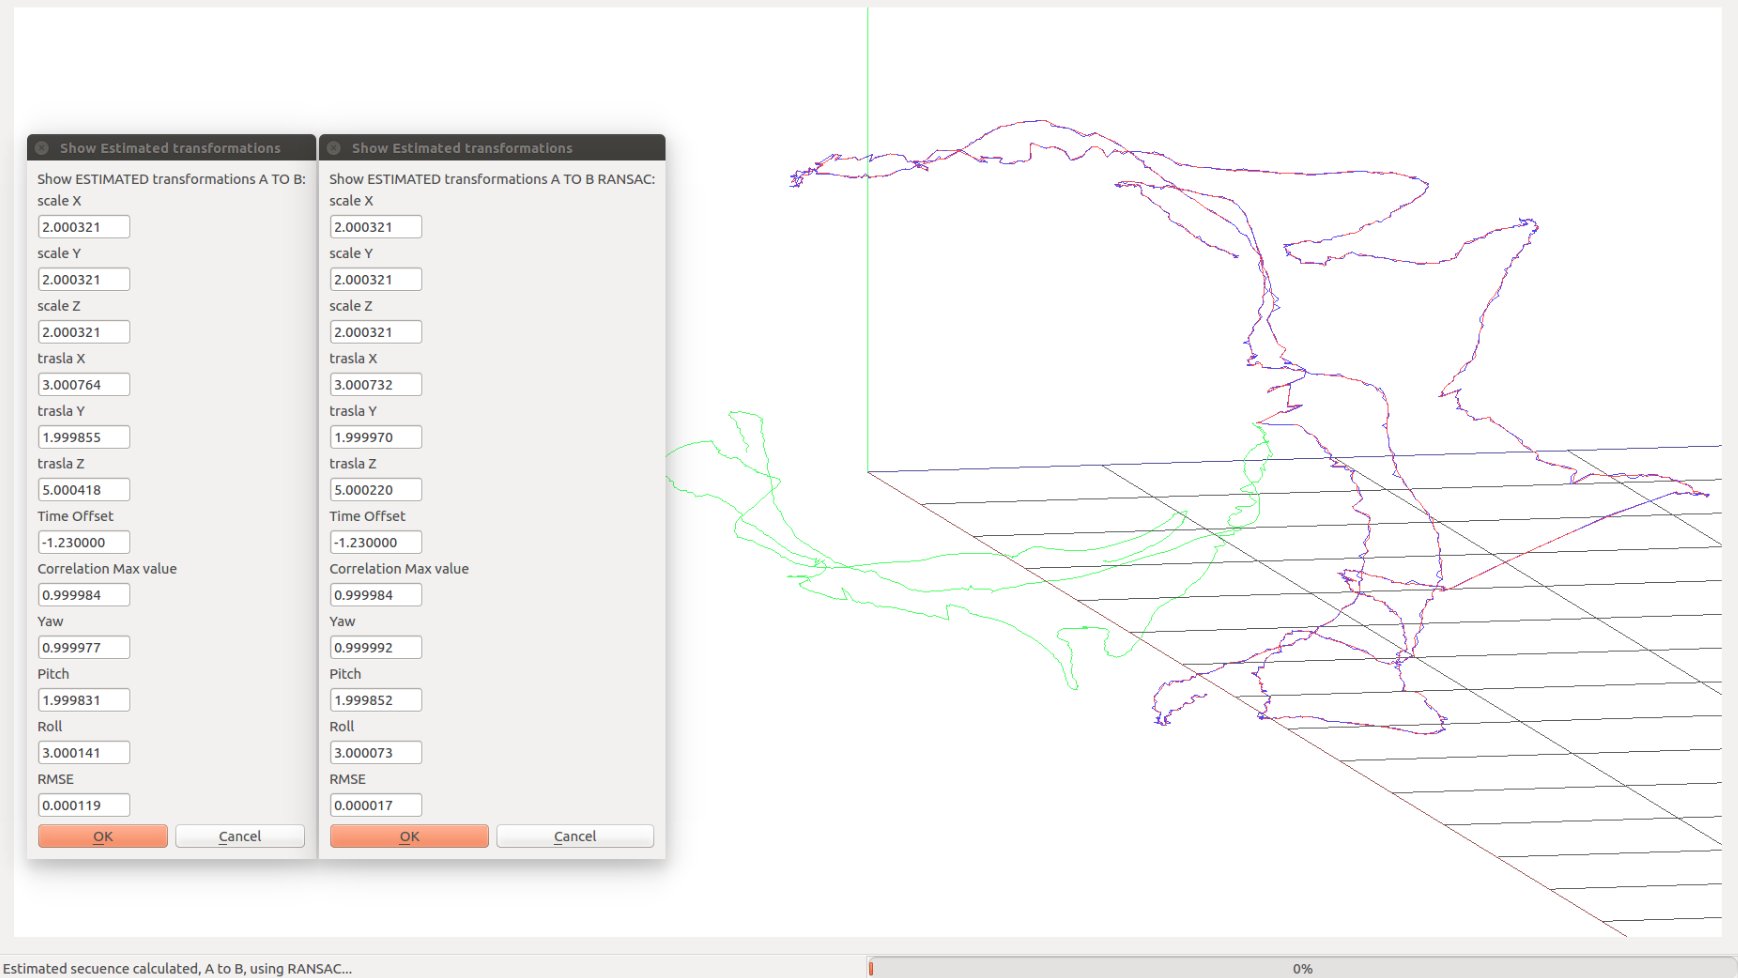
\includegraphics[height=14.0cm,width=18.0cm]{img/cap6/newData_EscalaTraslaRotaGauss_ab.png}
\hspace{0.5cm}

\end{center}


\caption{Resultados de la estimación B to A con ruido gaussiano y RANSAC}
\end{figure}

En la Figura 5.25, se ha añadido ruido gaussiano a las transformaciones anteriores y como consecuencia de aplicar este ruido hemos perdido algo de exactitud en los resultados.

El RMSE tiene un valor 0.000119 sin aplicar RANSAC y 0.000017 aplicando RANSAC, pero estos resultados siguen siendo muy próximos a 0.0 por tanto podemos decir que la estimación es muy buena.
El sentido de las estimaciones en la figura 5.25 es de dataset A a dataset B.


\begin{figure}[H]
\begin{center}
\label{fig:opciones de View}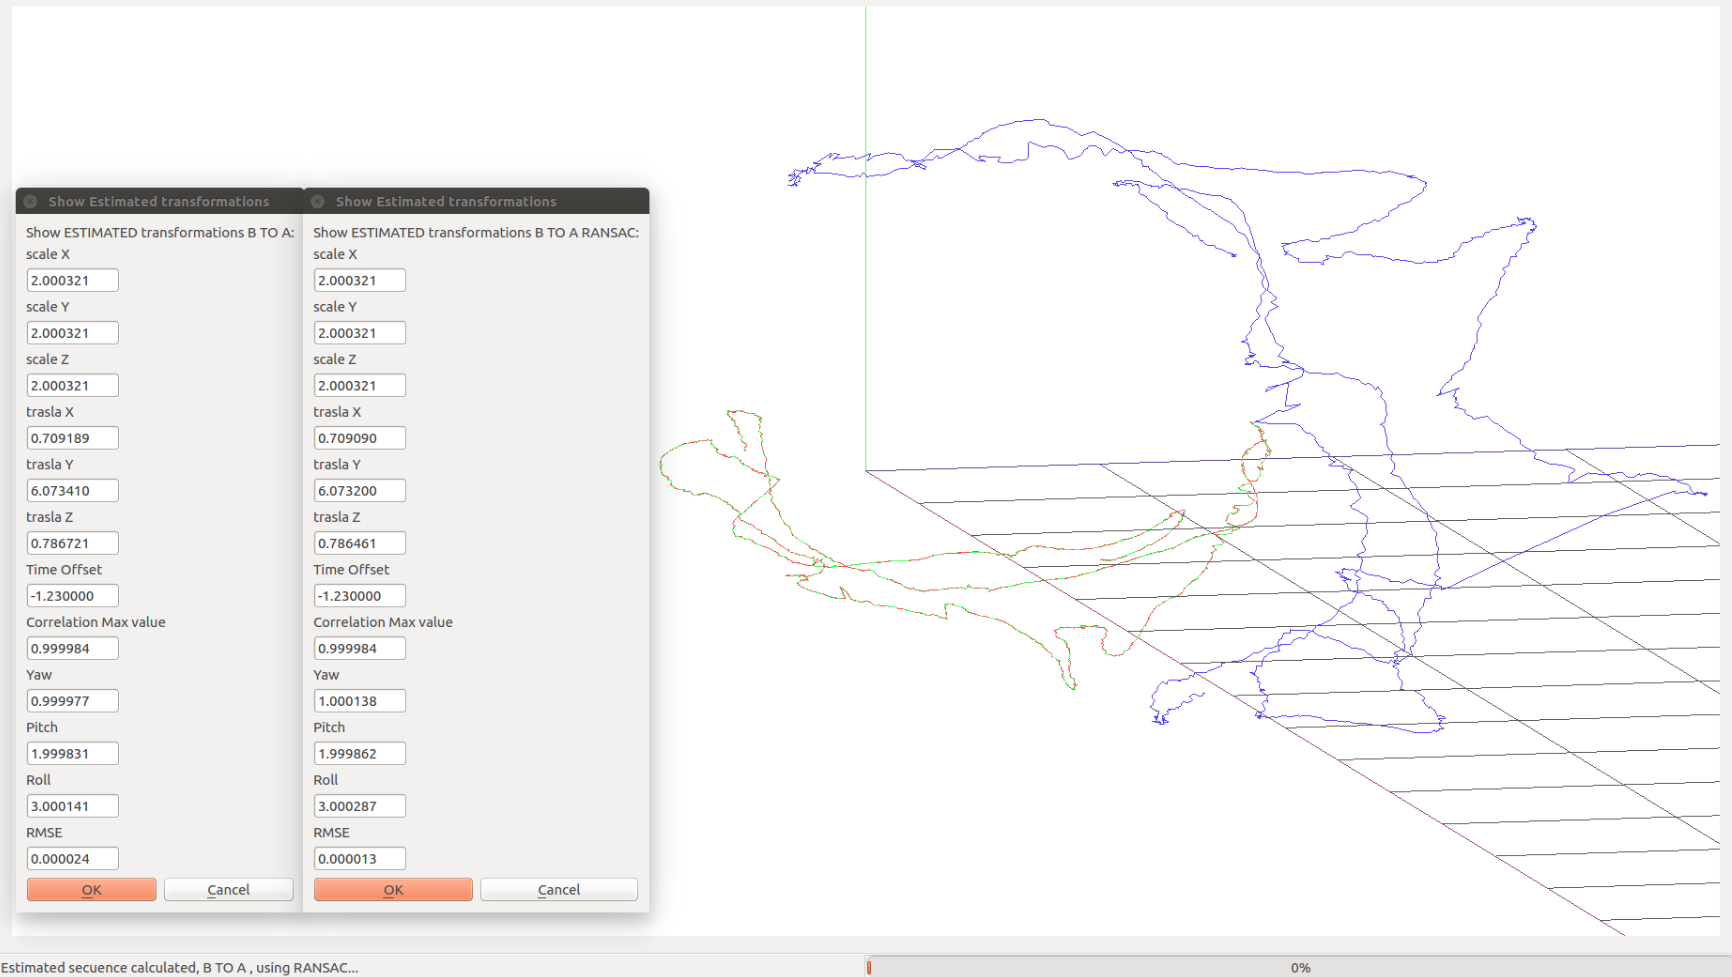
\includegraphics[height=14.0cm,width=18.0cm]{img/cap6/newData_EscalaTraslaRotaGauss_ba.png}
\hspace{0.5cm}

\end{center}

\caption{Resultados de la estimación B to A con ruido gaussiano y RANSAC}
\end{figure}
En la Figura 5.26, se ha añadido ruido gaussiano a las transformaciones anteriores y como consecuencia de aplicar este ruido hemos perdido algo de exactitud en los resultados.
El RMSE tiene un valor de 0.000024 sin aplicar RANSAC y 0.000013 aplicando RANSAC, pero estos resultados siguen siendo muy próximos a 0.0 por tanto podemos decir que la estimación es muy buena.
El sentido de las estimaciones en la figura 5.26 es de dataset B a dataset A.


\begin{figure}[H]
\begin{center}
\label{fig:opciones de View}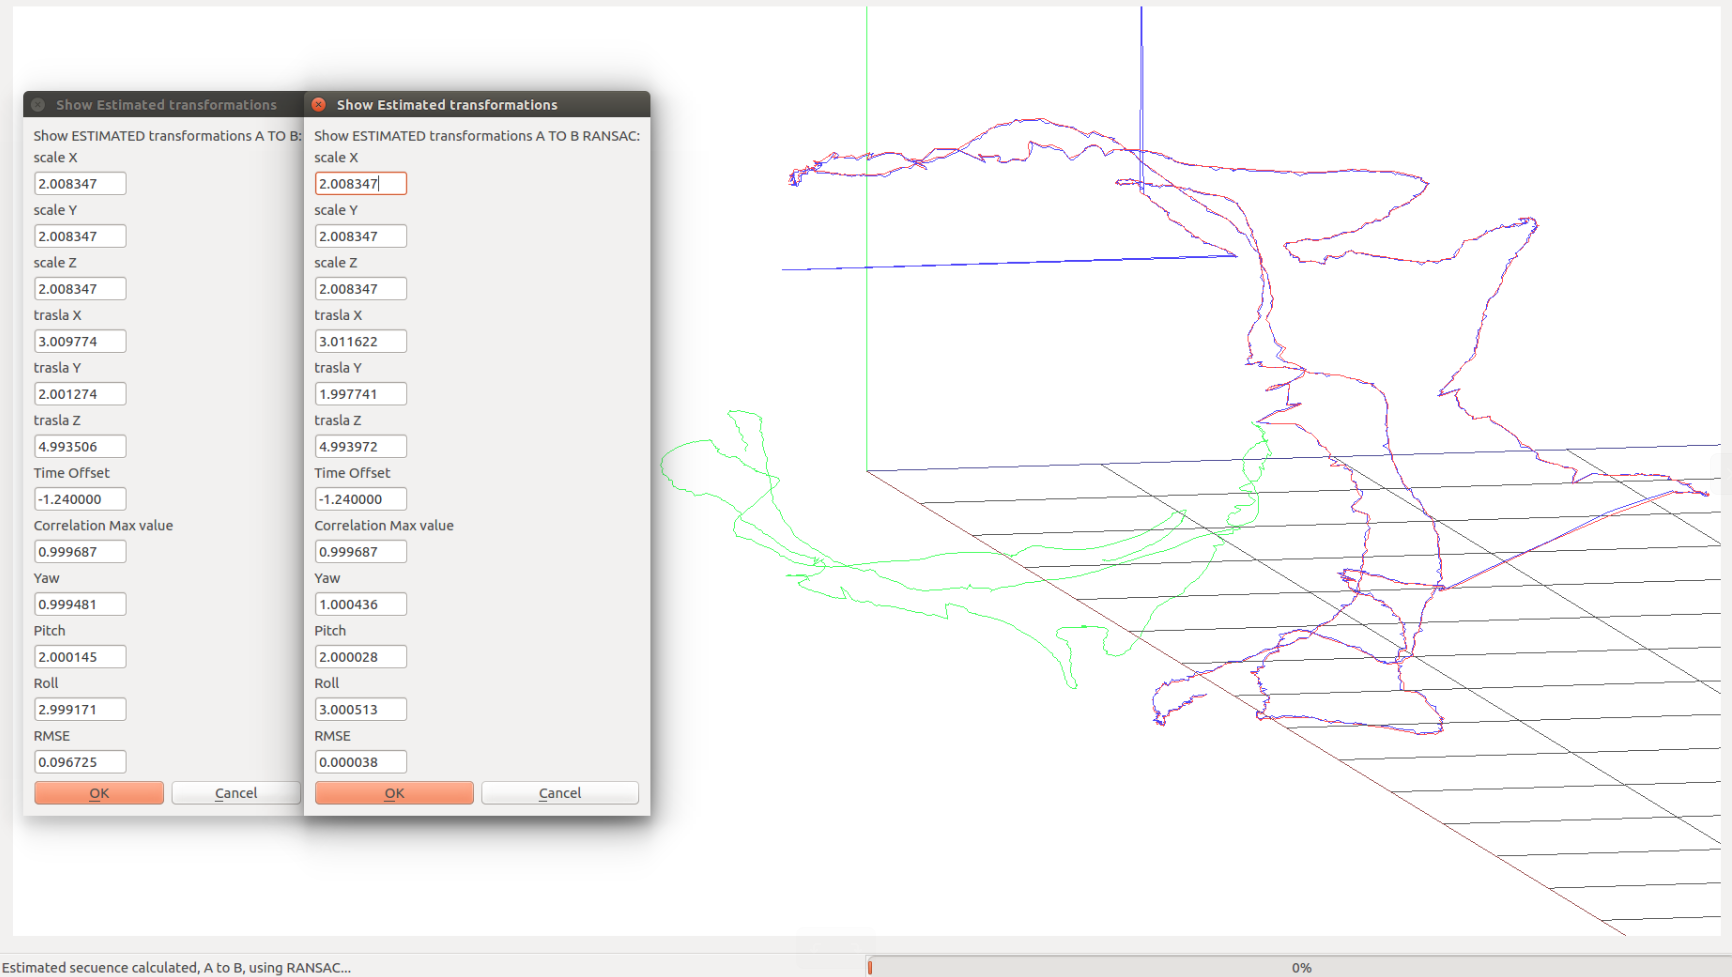
\includegraphics[height=14.0cm,width=18.0cm]{img/cap6/newData_EscalaTraslaRotaGaussCosmic_ab.png}
\hspace{0.5cm}
\end{center}

\caption{Resultados de la estimación A to B con ruido cósmico y RANSAC.}
\end{figure}
En la Figura 5.27, se ha añadido ruido gaussiano y ruido cósmico a las transformaciones anteriores y como consecuencia de añadir este ruido hemos perdido exactitud de manera notable en los resultados. 

El RMSE tiene un valor de 0.096725 sin aplicar RANSAC y 0.000038 aplicando RANSAC, en este caso los resultados son próximos a 0, pero nos acercamos a las décimas de error.
Además, el ruido cósmico ha afectado a la estimación del desplazamiento temporal, originalmente el valor era de 1,23 y se había estimado con exactitud en los casos anteriores, pero en este caso y con la presencia de ruido cósmico hemos estimado su valor en 1,24 , es decir hemos cometido un error de una centésima. Un error mayor cometido en la estimación del \textit{offset} temporal podría desajustar completamente el resto de estimaciones.
El sentido de las estimaciones en la figura 5.26 es de dataset A a dataset B.


\begin{figure}[H]
\begin{center}
\label{fig:opciones de View}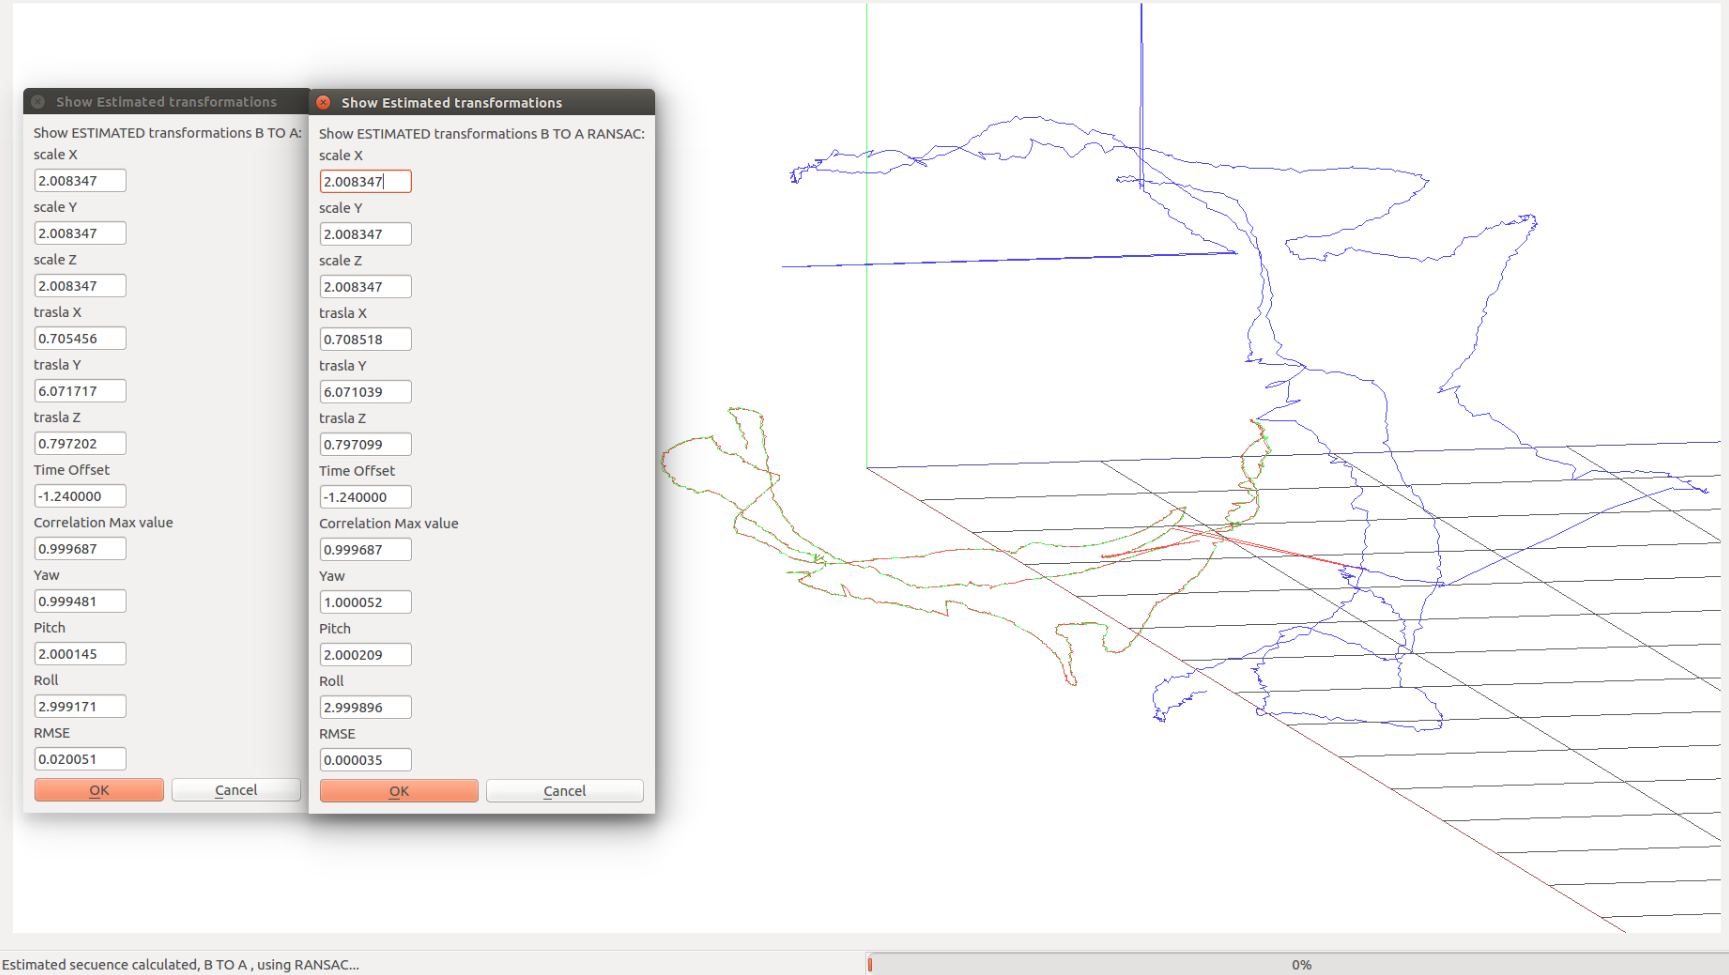
\includegraphics[height=14.0cm,width=18.0cm]{img/cap6/newData_EscalaTraslaRotaGaussCosmic_ba.png}
\hspace{0.5cm}
\end{center}

\caption{Resultados de la estimaciones B to A con ruido cósmico y RANSAC.}
\end{figure}
En la Figura 5.28, se ha añadido ruido gaussiano y ruido cósmico a las transformaciones anteriores y como consecuencia se ha perdido exactitud de manera notable en los resultados. 
El RMSE tiene un valor de 0.020051 sin aplicar RANSAC y 0.000035 aplicando RANSAC, en este caso los resultados son próximos a 0, pero nos acercamos a las décimas de error.
También en este caso comprobamos que el ruido cósmico ha afectado a la estimación del desplazamiento temporal, originalmente el valor era de 1,23 y se había estimado con exactitud en los casos anteriores, pero en este caso y con la presencia de ruido cósmico hemos estimado su valor en 1,24, es decir hemos cometido un error de una centésima.
El sentido de las estimaciones en la figura 5.26 es de dataset B a dataset A.


Los experimentos anteriores han demostrado que la herramienta desarrollada es precisa para todo tipo de transformaciones, obteniendo un error máximo de 0.02 (sálvo en presencia de ruido cósmico). Las transformaciones que más perjudican a las estimaciones realizadas son las que contiene ruido gaussiano (ruido leve) y especialmente ruido cósmico cuyos valores pueden llegar a distorsionar notablemente los datos (en alguna ocasión, en presencia de ruido cósmico, hemos obtenido un RMSE = 0.2 ) ya que introducen valores aleatorios en el dataset que no se corresponden con la distribución de los valores del dataset. En este caso, cuando el dataset está contaminado con este tipo de ruidos se ha comprobado que la utilización de los algoritmos RANSAC son adecuados para eliminar datos espúreos y ajustar mejor el dataset estimado al \textit{groundtruth}.

Aun así, estos errores son lo suficientemente pequeños como para que se utilice esta herramienta para validar la precisión de los algoritmos de Visual SLAM.



\clearpage
\newpage





%\begin{figure}[H]
%\begin{center}
%\subfigure[]{\label{fig:opciones de View}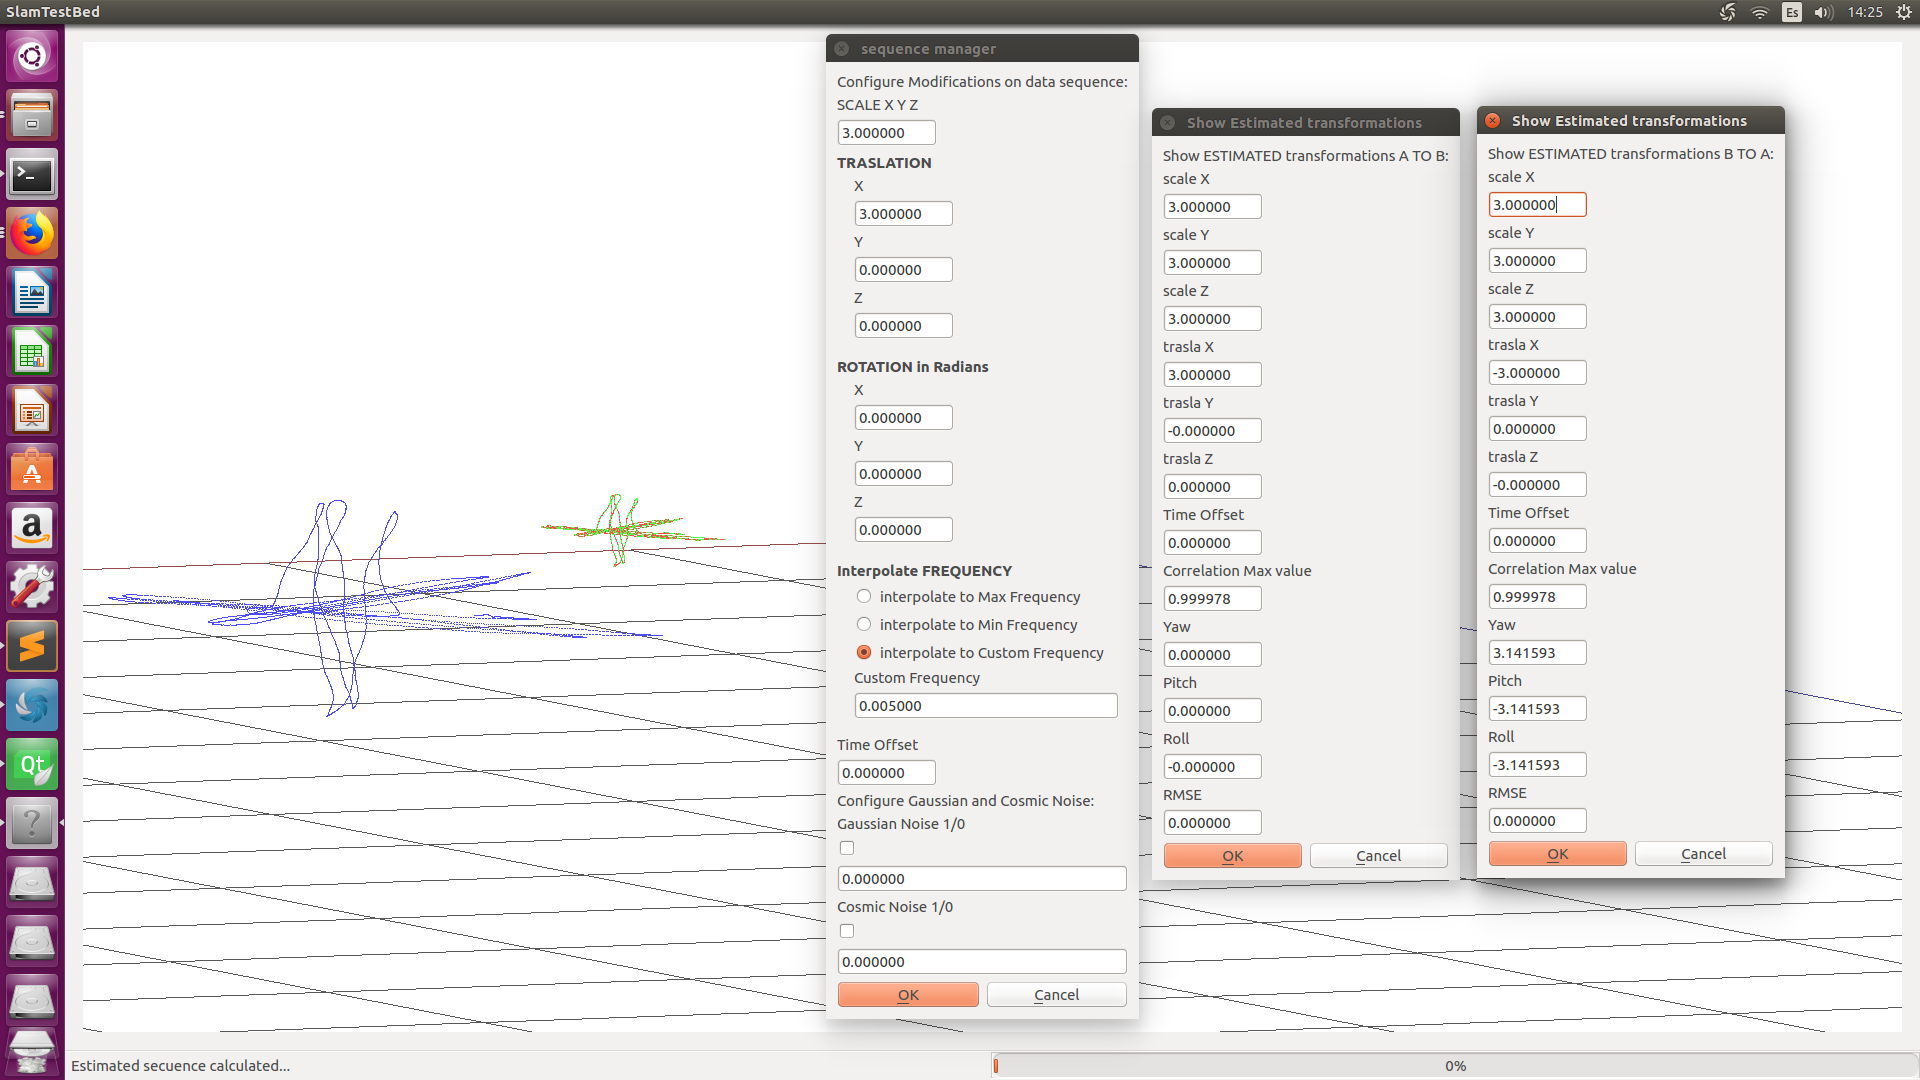
\includegraphics[height=8.0cm,width=12.0cm]{img/cap6/ScaleTraslaFrec.png}}
%\hspace{0.5cm}

%\end{center}

%\caption{Gráfico que muestra los resultados de la estimación de un cambio de escala, traslación y frecuencia.}
%\end{figure}


%\begin{figure}[h][H]
%\begin{center}
%\subfigure[]{\label{fig:opciones de View}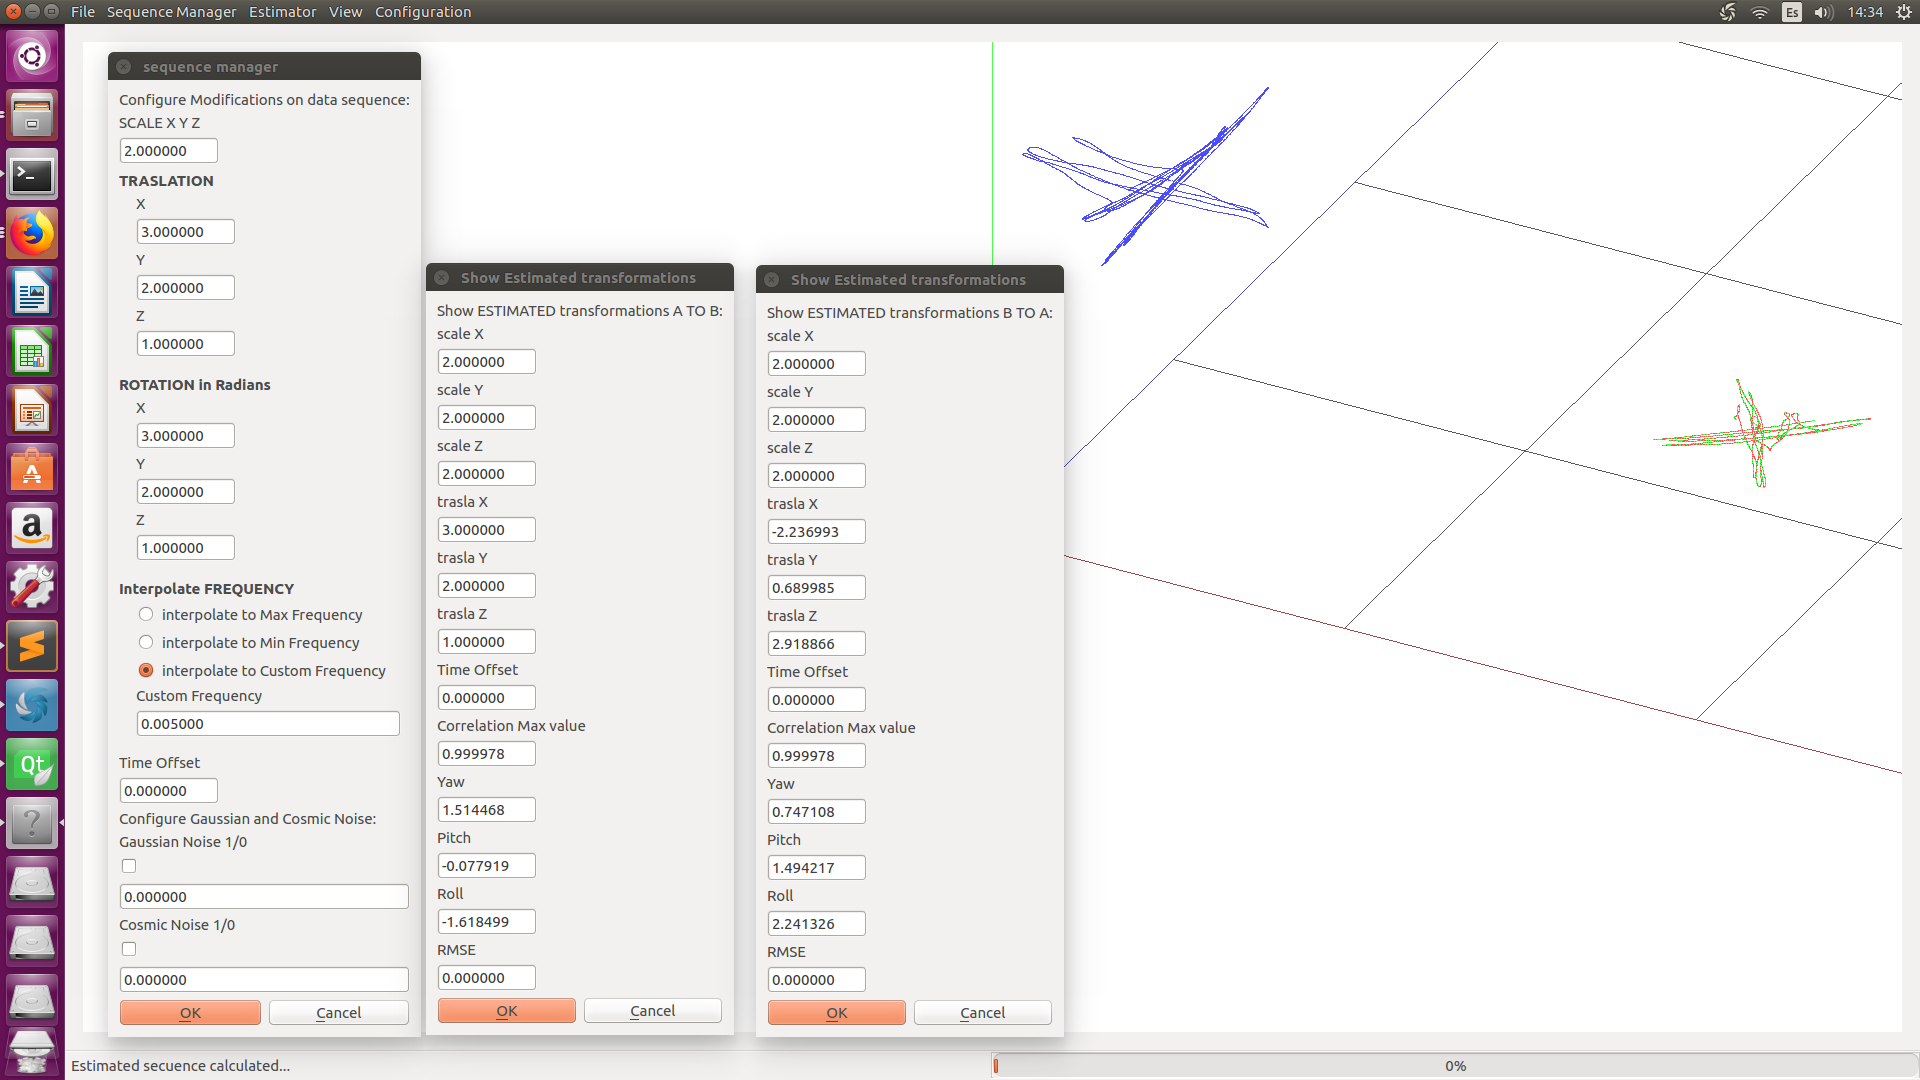
\includegraphics[height=8.0cm,width=12.0cm]{img/cap6/ScaleTraslaRotaFrec.png}}
%\hspace{0.5cm}

%\end{center}

%\caption{Gráfico que muestra los resultados de la estimación de un cambio de escala, traslación,rotación y frecuencia.}
%\end{figure}


%\begin{figure}[H]
%\begin{center}
%\subfigure[]{\label{fig:opciones de View}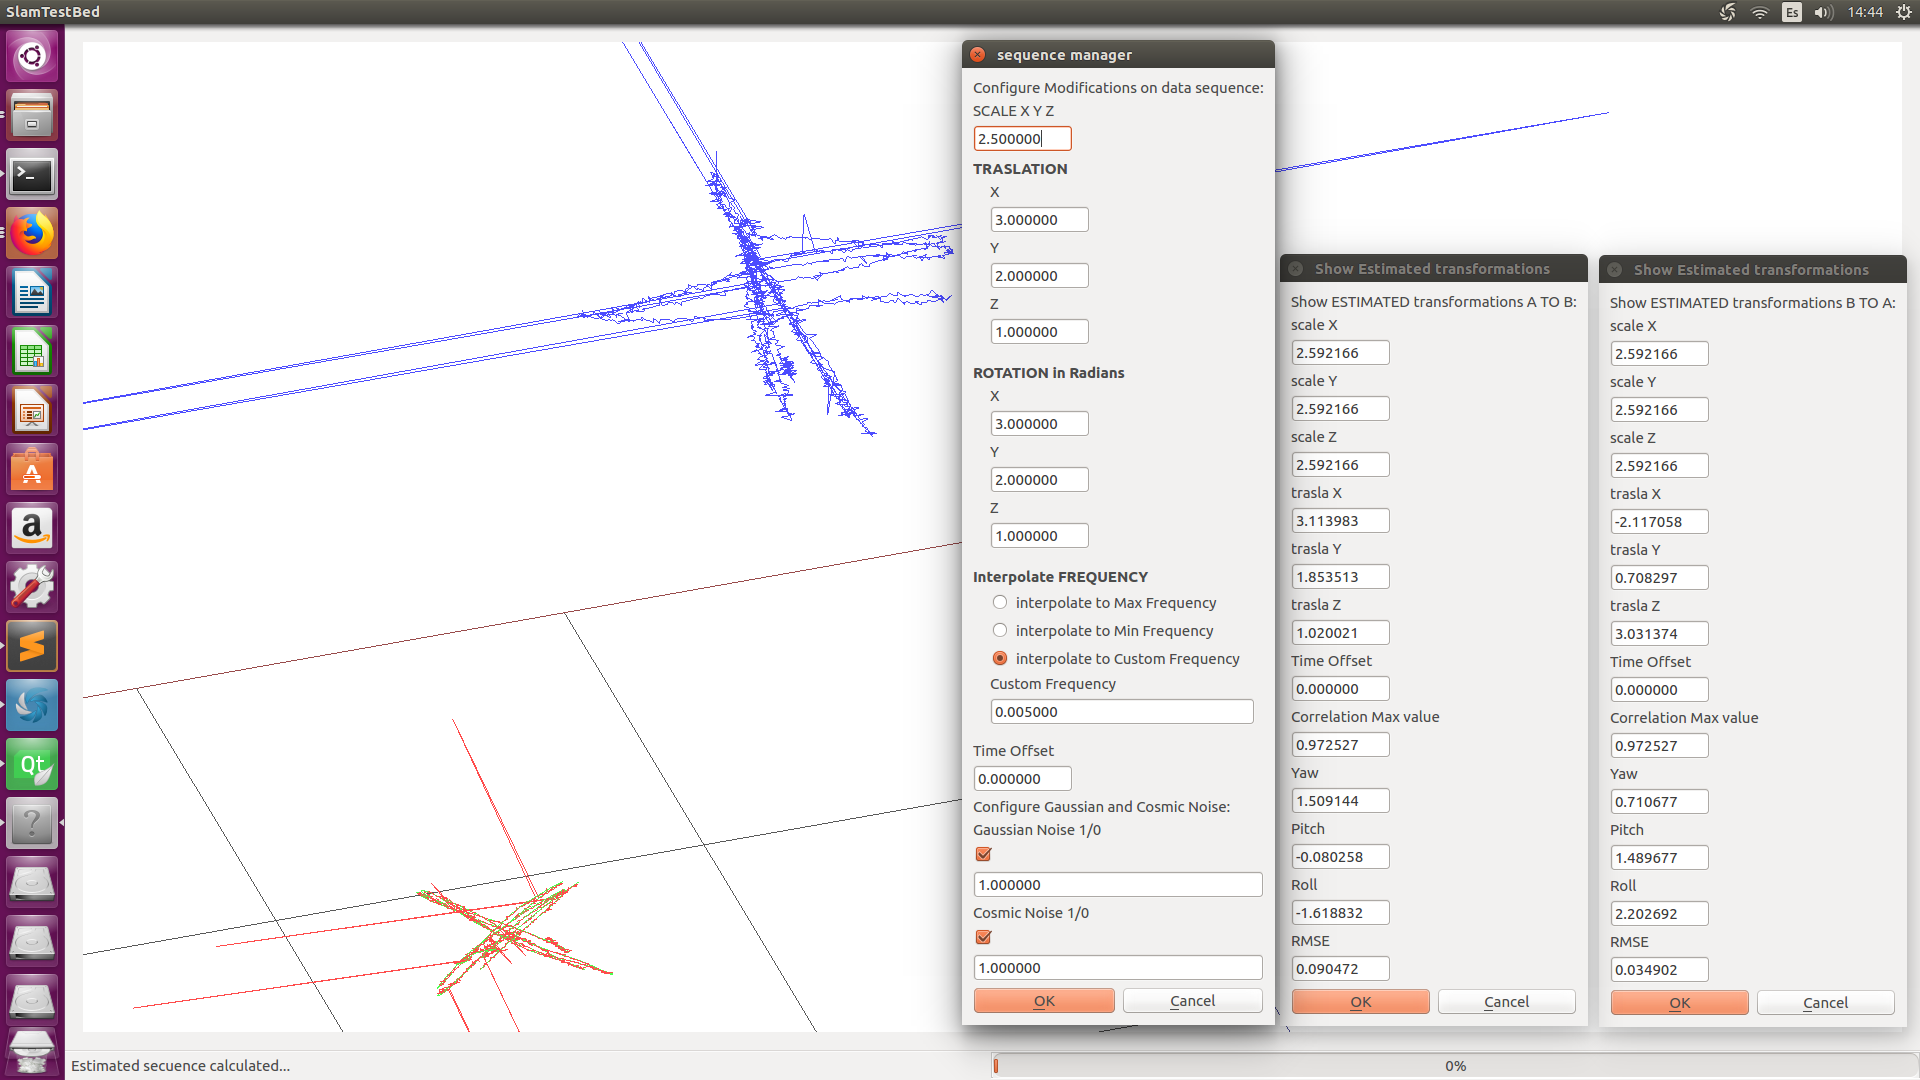
\includegraphics[height=8.0cm,width=12.0cm]{img/cap6/ScaleTraslaRotaFrecGNoiseCNoise.png}}
%\hspace{0.5cm}

%\end{center}

%\caption{Gráfico que muestra los resultados de la estimación de un cambio de escala, traslación, rotación, frecuencia, ruido gaussiano y ruido cósmico.}
%\end{figure}



%\begin{figure}[h][H]
%\begin{center}
%\subfigure[]{\label{fig:opciones de View}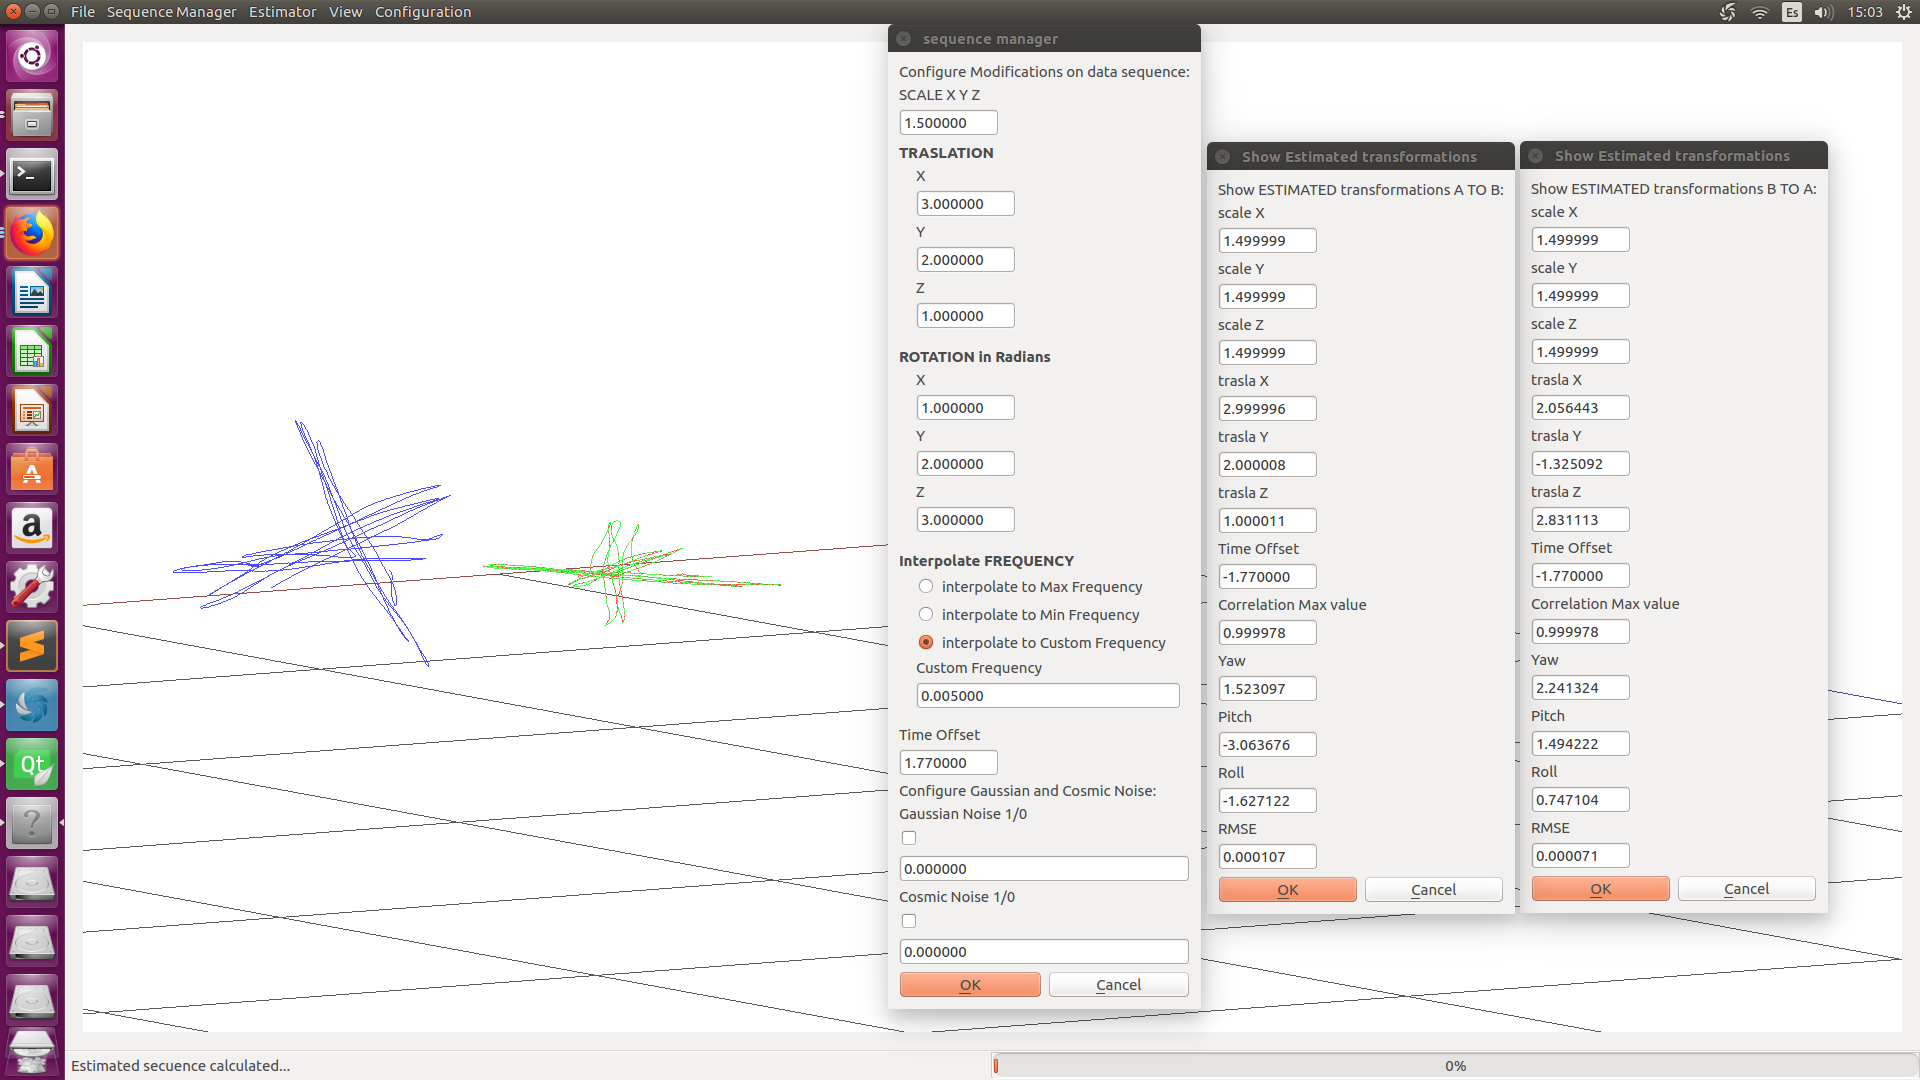
\includegraphics[height=8.0cm,width=12.0cm]{img/cap6/ScaleTraslaRotaFrecTimeOffset.png}}
%\hspace{0.5cm}

%\end{center}

%\caption{Gráfico que muestra los resultados de la estimación de un cambio de escala, traslación, rotación, frecuencia y offset.}
%\end{figure}


%\begin{figure}[H]
%\begin{center}
%\subfigure[]{\label{fig:opciones de View}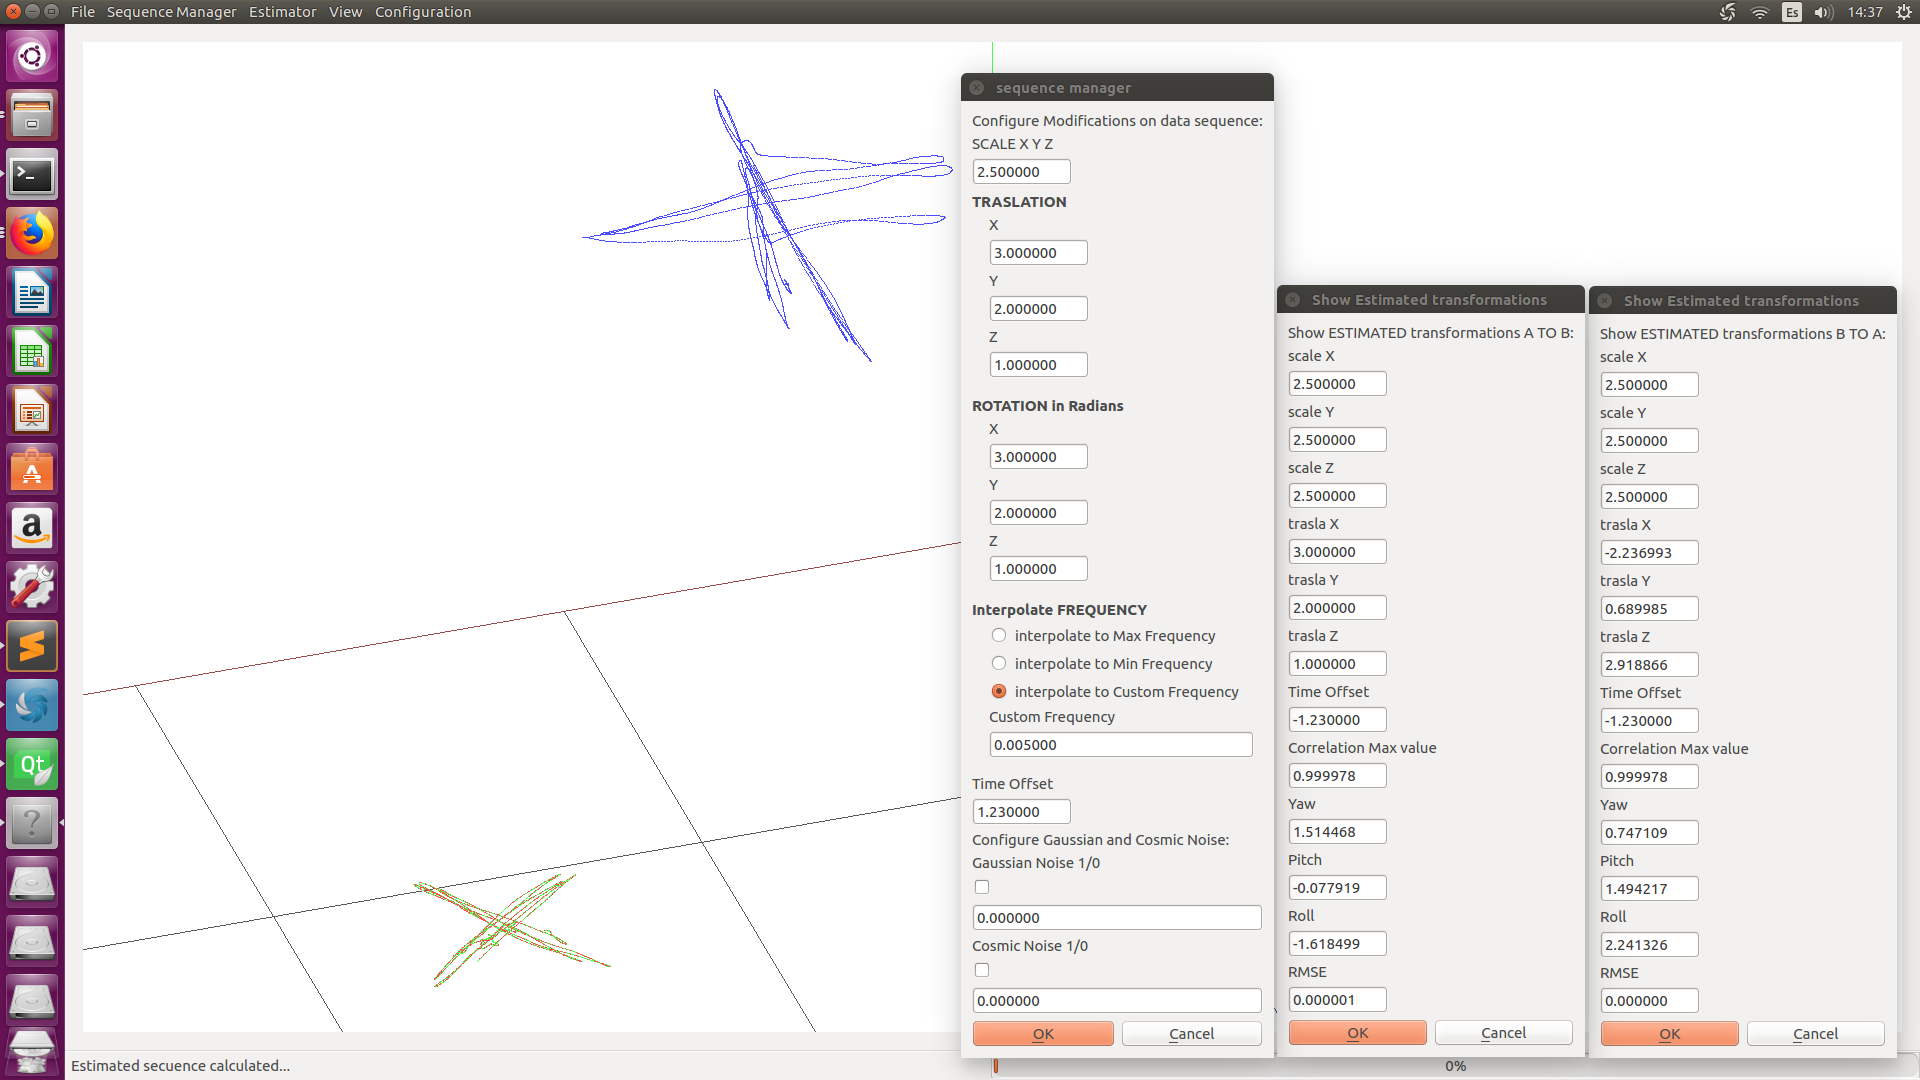
\includegraphics[height=8.0cm,width=12.0cm]{img/cap6/ScaleTraslaRotaFrecTimeOffset2.png}}
%\hspace{0.5cm}

%\end{center}

%\caption{Gráfico que muestra los resultados de la estimación de un cambio de escala, traslación, rotación, frecuencia y offset.}
%\end{figure}



%\begin{figure}[h][H]
%\begin{center}
%\subfigure[]{\label{fig:opciones de View}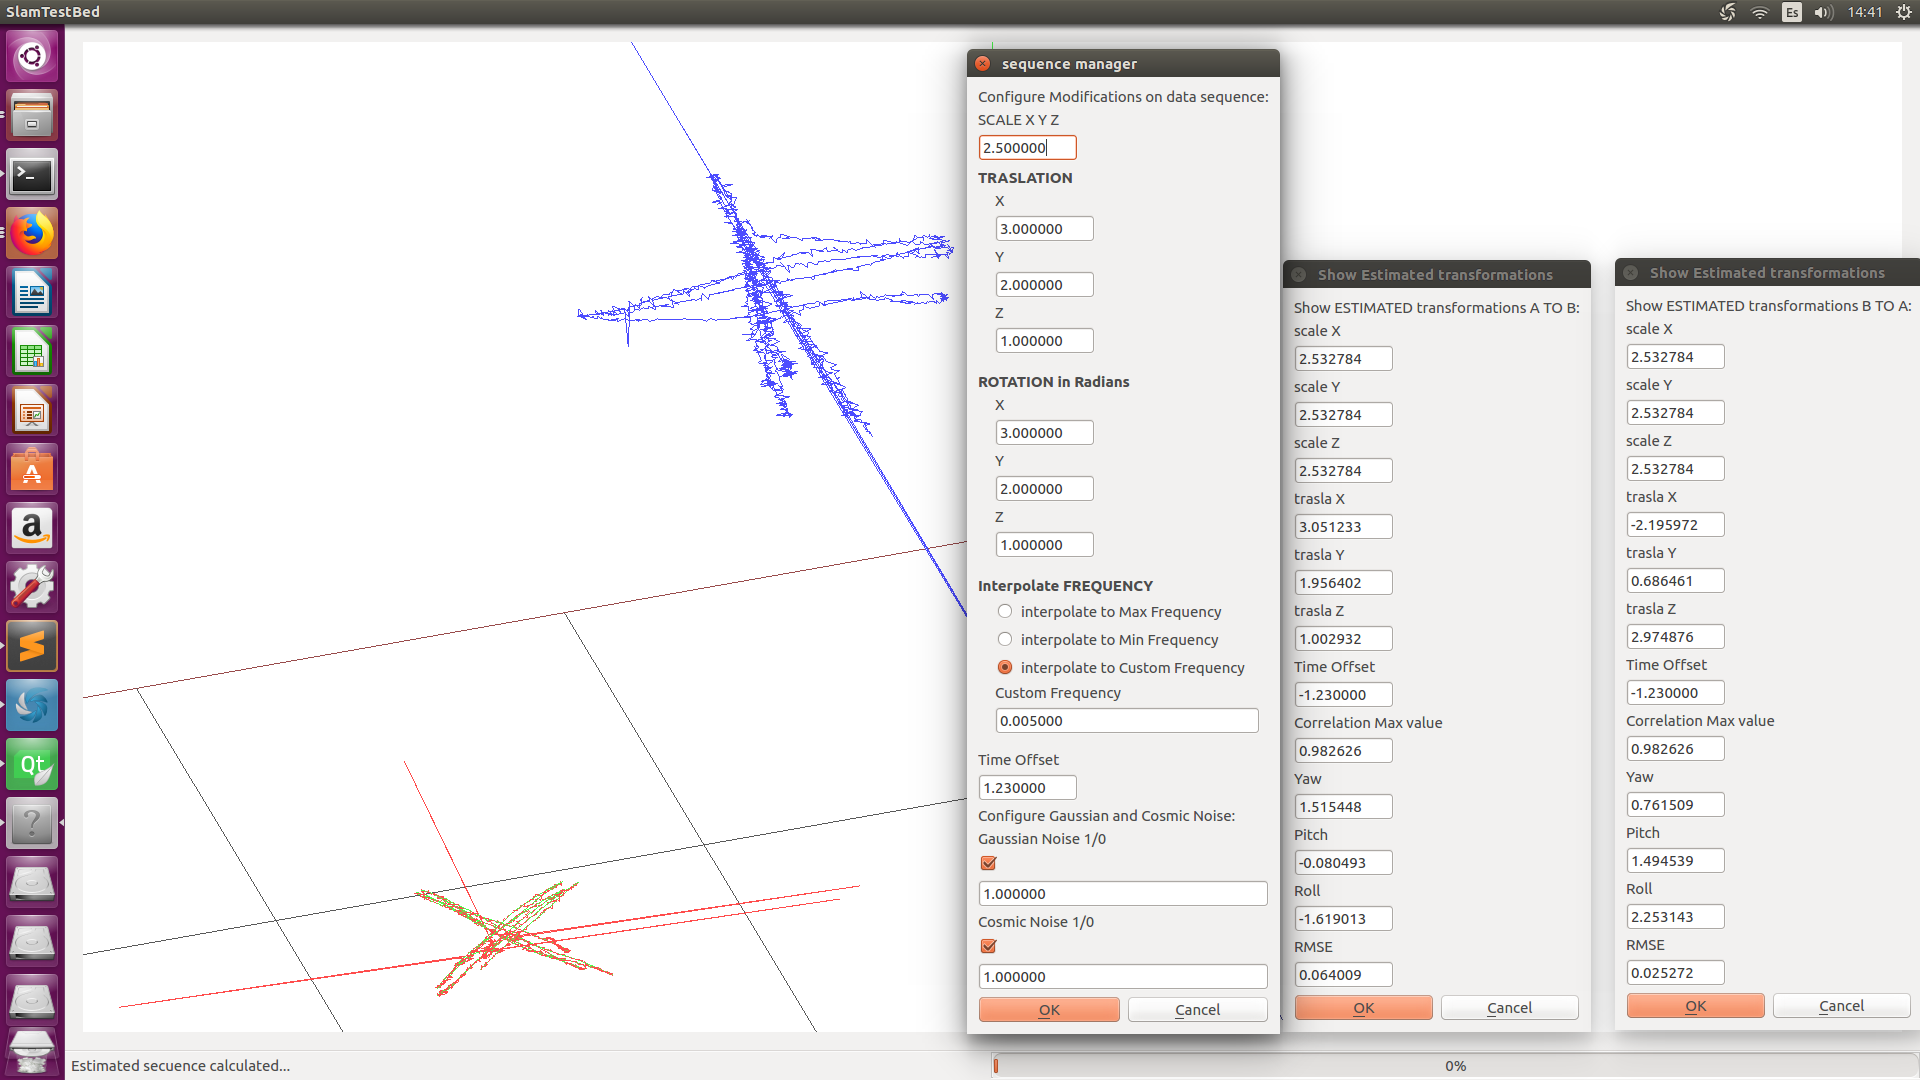
\includegraphics[height=8.0cm,width=12.0cm]{img/cap6/ScaleTraslaRotaFrecTimeOffsetGNoiseCNoise.png}}
%\hspace{0.5cm}

%\end{center}

%\caption{Gráfico que muestra los resultados de la estimación de un cambio de escala, traslación, rotación, frecuencia, Offset, Ruido Gaussiano y Ruido Cósmico.}
%\end{figure}




%\begin{figure}[H]
%\begin{center}
%\subfigure[]{\label{fig:opciones de View}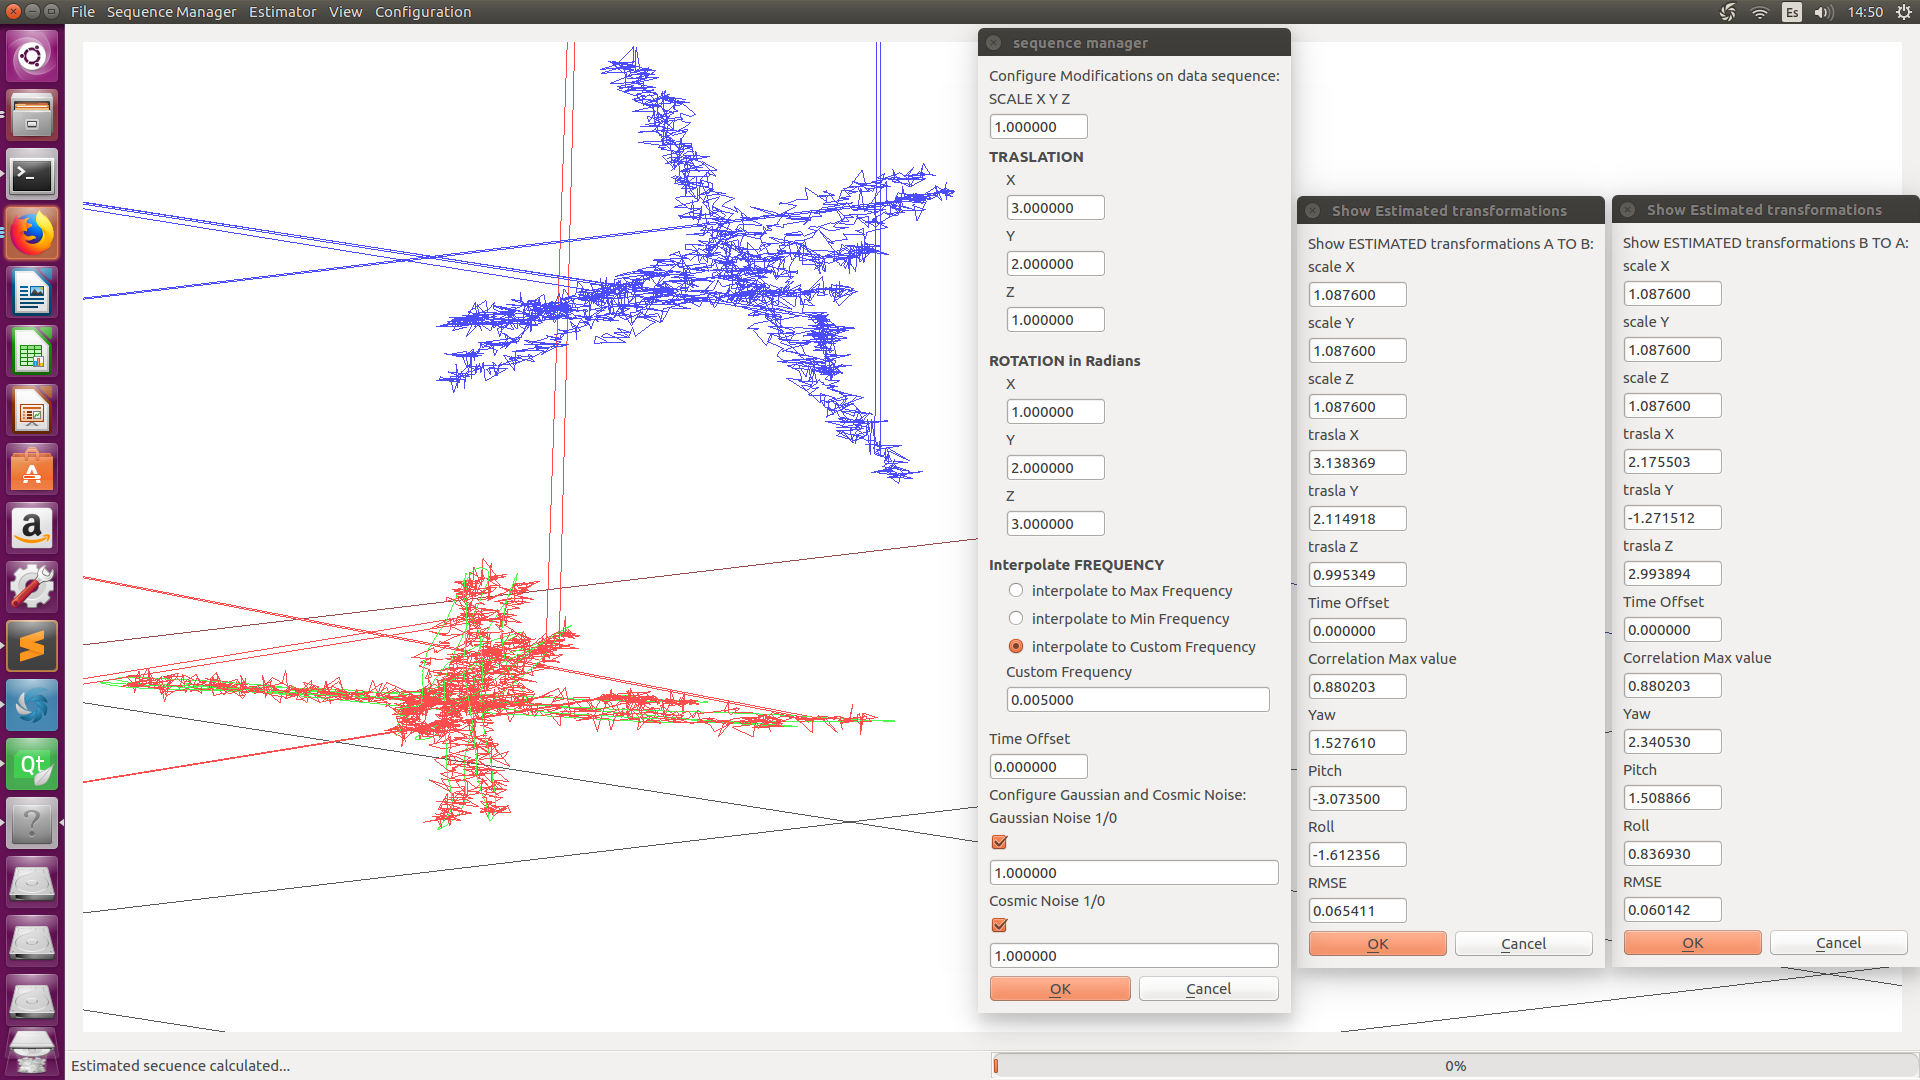
\includegraphics[height=8.0cm,width=12.0cm]{img/cap6/TraslaRotaFrecGnoiseCnoise.png}}
%\hspace{0.5cm}

%\end{center}

%\caption{Gráfico que muestra los resultados de la estimación de un cambio de traslación, rotación, frecuencia, Ruido Gaussiano y Ruido Cósmico.}
%\end{figure}


%Por último también mostraremos como SLAMTestBed es capaz de operar con 2 datasets diferentes , es decir en este caso , el segundo dataset no será el resultado de aplicar el módulo %de transformación sobre el primer dataset.

%\begin{figure}[h][H]
%\begin{center}
%\subfigure[]{\label{fig:opciones de View}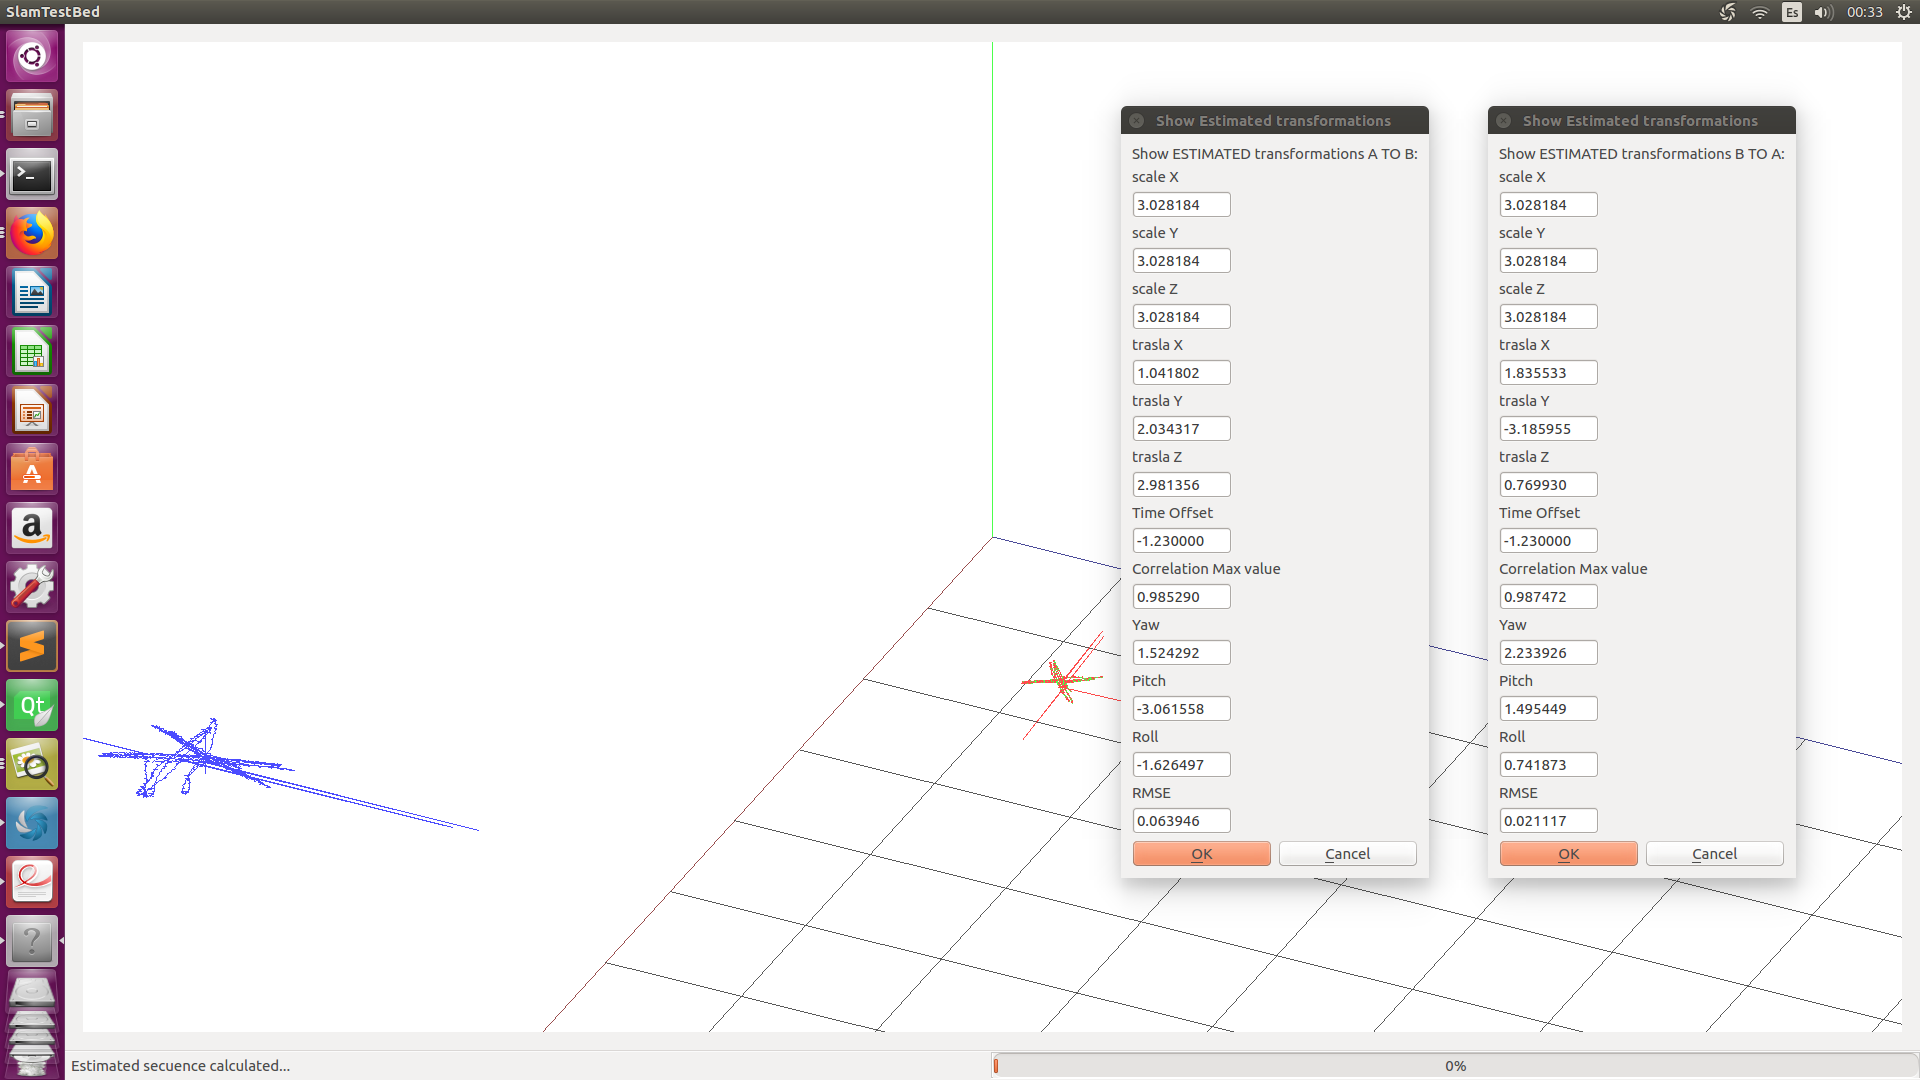
\includegraphics[height=8.0cm,width=12.0cm]{img/cap6/LoadTwoDataSets.png}}
%\hspace{0.5cm}

%\end{center}

%\caption{Gráfico que muestra los resultados de la estimación de la transformación del dataSet A en el datasetB y viceversa.}
%\end{figure}


%\begin{figure}[H]
%\begin{center}
%\subfigure[]{\label{fig:opciones de View}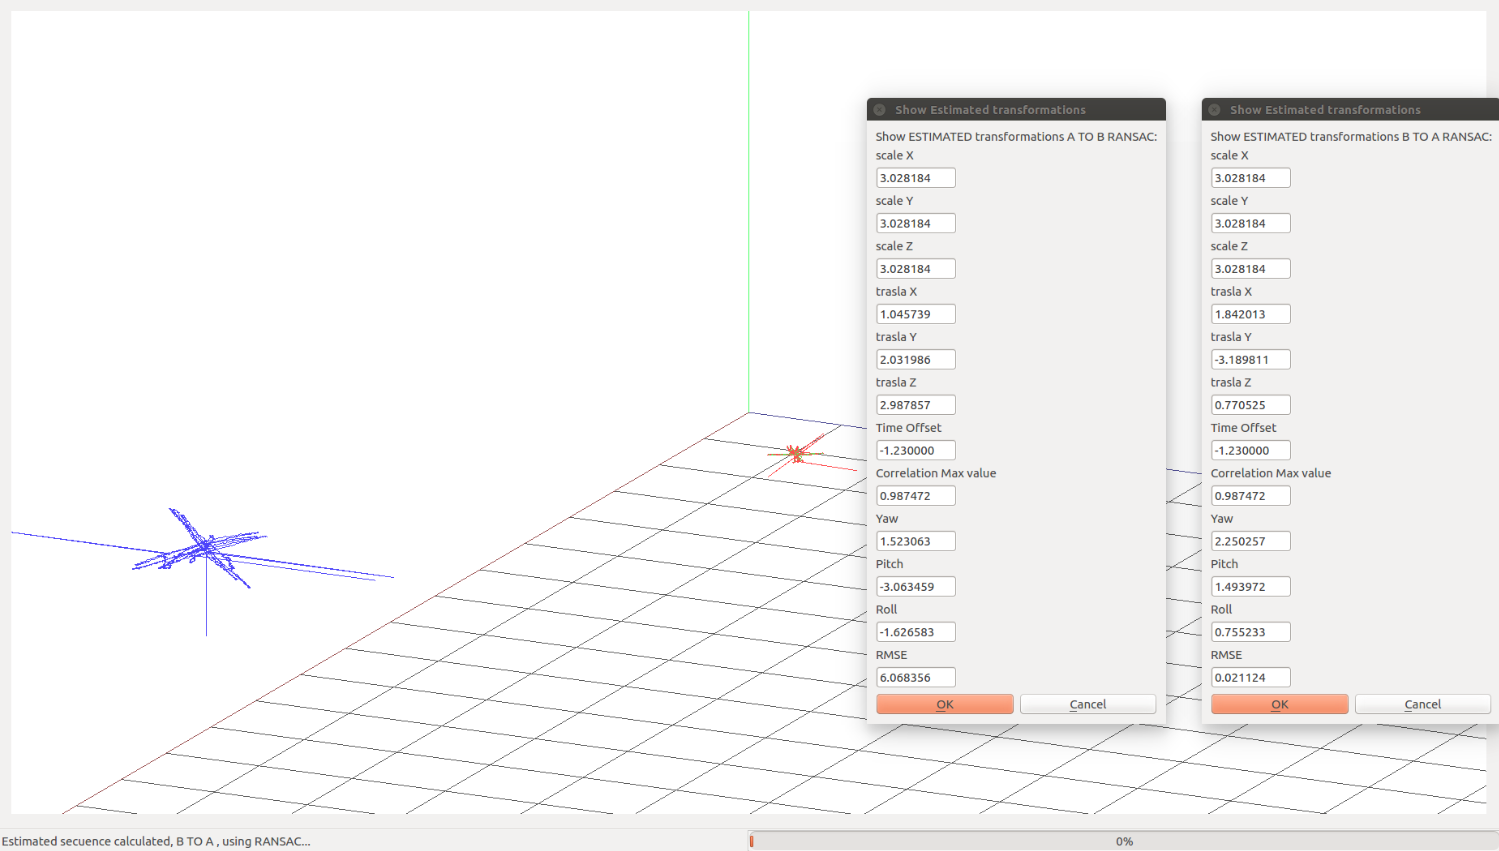
\includegraphics[height=8.0cm,width=12.0cm]{img/cap6/LoadTwoDataSets_RANSAC.png}}
%\hspace{0.5cm}

%\end{center}

%\caption{Gráfico que muestra los resultados de la estimación de la transformación del dataSet A en el datasetB y viceversa, utilizando RANSAC.}
%\end{figure}

%\clearpage


